
Writing for peer-reviewed publication is an important part of the careers of many scientists and engineers. It is also an essential part of the scientific enterprise. Something this important should be done well. However, many scientists and engineers do not consider themselves good writers, so how can the average scientist write a good scientific paper?

The good news is you do not have to be a good writer to write a good science paper, but you do have to be a careful writer. And while the creativity that often marks good science will sometimes spill over into the writing about that science, in general, good science writing does not require creative writing. In particular, writing for a peer-reviewed science or engineering journal requires learning and executing a specific formula for presenting scientific work.

This book is all about teaching the style and conventions of writing for a peerreviewed science journal. (For the sake of brevity, I will use the word "science" to mean both science and engineering.) Anyone who absorbs the lessons of this book can become a better writer. At the least, you can become a good enough writer that your readers will judge your work by the quality of the science rather than the quality of the writing.

What I know about science writing has come from three separate experiences. First, I have written over 200 papers in my $30+$-year career in the semiconductor industry. Like most authors, I have become a better writer through practice. I have also spent the last six years as Editor-in-Chief of the Journal of Micro/Nanolithography, MEMS, and MOEMS $\left(\mathrm{JM}^{3}\right)$, published by SPIE. That experience has forced me to judge the writing of others and to see the good, the bad, and the ugly of science publishing. Because of this experience, I embarked on a project of studying what makes for good science writing, and I have read many papers and books by other writers, editors, and historians of science on that topic. Taking advantage of my post as Editor-in-Chief, I started writing a series of editorials in $\mathrm{JM}^{3}$ on good science writing (2012-2018). This book is mostly a compilation of those editorials.

\section*{The Three Pillars of Science}
Science can be thought of as the combination of three essential things: (1) a communal collection of knowledge (both facts/data and theories); (2) a method of evaluating the efficacy of scientific theories by comparing the predictions of those theories to observation/experiment; and (3) an attitude of skeptical inquiry and the belief that all scientific knowledge is provisional and subject to revision when confronted with new evidence. (A popular alternative breakdown of the "norms" of science, emphasizing its sociological nature, is Merton's "cudos", first introduced in 1942: communalism, universality, disinterestedness, originality, and skepticism. ${ }^{1}$ ) This breakdown of science into a body of knowledge, a method, and an attitude is useful in assessing the "scientific" content of any given behavior. If any one of these three pillars of science is missing from an activity, one cannot claim that the activity is scientific.

The growth of scientific knowledge is

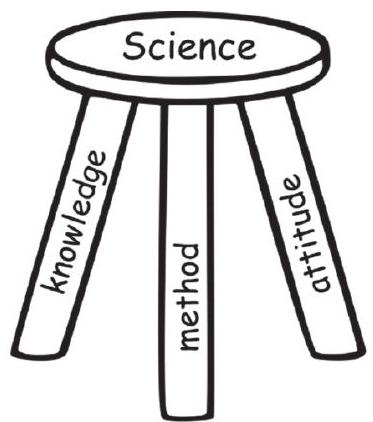
\includegraphics[max width=\textwidth, center]{2024_04_11_419211c3e451fc7cea07g-002}
predominately incremental — we build on past knowledge more often than we displace it. Thus, the first pillar of science-a communal collection of knowledge-requires mechanisms for disseminating and preserving knowledge within the scientific community. By far the most important mechanism in use today is the scientific publication. Although there are many forms of scientific publication, the most important is the peer-reviewed journal paper. The goal of this book is to help authors produce good scientific papers and thus support the goals of science.

\section*{Using This Book}
This book can be read straight through, which I recommend for early-career scientists who are relatively new to writing and publishing papers. It can also be used as a reference for specific topics (e.g., how to produce a good figure or write an abstract). Each chapter is purposely short and can be read in isolation for easy reference. The appendix - a checklist for editors, reviewers, and authors - is a summary of the lessons of this book.

Throughout this book I will use the words "science" and "scientist" in the most expansive way possible to include people and activities generally called "engineering." Publishing in highly practical engineering fields or highly theoretical science fields (and every part of the continuum in between) has mostly the same requirements. Some fields, such as medicine, include additional important requirements, especially related to the use of and reporting on human or animal subjects. I will not be covering those important topics in this book, but the general lessons here apply even to those more specialized fields.

Because of my experience as Editor-in-Chief of $\mathrm{JM}^{3}$, I have intimate knowledge and insider information about this specific journal. Where useful, I have included specific information from $\mathrm{JM}^{3}$ to use as examples of the points  make in the book. $\mathrm{JM}^{3}$ is probably representative of journals positioned halfway between pure science and pure engineering, and I hope that examples from this journal will make the lessons of this book more real.

\section*{Acknowledgments}
My learning about science writing leaves me with many debts of gratitude. The experience of writing, for me, had been a mostly joyful and satisfying one. I am indebted to the many good authors who I have read and to the many coauthors I have been privileged to write with. Less pleasant have been the rejection letters and difficult reviews that I have received over the years, but I am even more indebted to these editors and reviewers for their careful and constructive criticisms that forced me to improve even when I did not want to. I am also grateful for the readers of my books and articles who have given me feedback and asked me questions. They have taught me that when a reader does not understand what I have written, it is almost always my fault, not theirs.

I would also like to thank the volunteer scientists that make up the editorial board of $\mathrm{JM}^{3}$. Together, we have gone through the sometimes exciting but often routine process of publishing a peer-reviewed science journal issue after issue. Finally, I would like to thank the wonderful staff of SPIE, who not only publish $\mathrm{JM}^{3}$ but are also publishing this book and making it freely available in electronic format. I have learned a tremendous amount from Eric Pepper and Karolyn Labes, who have coached and mentored me in my role as Editor-in-Chief and have reviewed and improved all of the material in this book. Thanks to John Mays and Scott McNeill as well for reviewing the text of this book.

I conclude with these oft-repeated words: much of what is good in this book is a consequence of the many people who have helped me over the years, and all of what is bad is due to my own shortcomings.

Chris A. Mack

Austin, Texas

January 2018

\section*{References}
\footnotetext{${ }^{1}$ R. K. Merton, The Sociology of Science: Theoretical and Empirical Investigations, University of Chicago Press, Chicago, IL (1973).
}
\section*{Chapter 1}
\section*{Getting Started}
If you are thinking about writing a science paper for peer review and publication, what should be your first steps? Ideally, you have thought about the possibility of writing and publishing early in your research project because some early planning can help you avoid problems later. But first, you should ask yourself about your motivations for writing a science paper.

\subsection*{1.1 Why Write and Publish a Paper?}
Writing a paper and getting it published in a peer-reviewed journal is hard work, even after the hard work that led to the publishable results. So why do people do it? What motivates authors to go through the writing process, and then the peer review process, in order to publish their work? There are two kinds of motivations, altruism and self-interest, and most authors have some combination of the two.

\section*{Altruism}
Peer-reviewed science publications are the predominant method today for disseminating and archiving scientific advances (books, conference presentations, and university teaching are other common ways). Science grows and advances through a communal collection of knowledge that is constantly being challenged, revised, and expanded. ${ }^{1,2}$ Most scientists (and I include engineering in the broadest sense of science) have a strong desire to contribute to the advancement of their field, which is often their primary reason for becoming a scientist. Publication is usually the most straightforward way to make such a contribution, and it is thus highly motivating (and satisfying) to most scientists.

\section*{Self-Interest}
Publishing can also bring tangible benefits to an author, thus providing a selfinterested motivation for writing and publishing a paper. Publishing may be required for career advancement and is frequently accompanied by direct or indirect monetary rewards. The familiar "publish or perish" paradigm in academia adds a proverbial stick to the carrot of career advancement. But even without these obvious professional motivations, almost all human beings crave recognition for their efforts. I know that I am highly motivated by the reward of peer recognition;

I am gratified to see my worked used and referenced, and I take pride in publishing in journals that I respect and admire.

\section*{Balancing Altruism and Self-Interest}
Let me be clear that I do not view self-interested motivations as inherently bad or even fundamentally worse than altruistic motivations. Any properly regulated and well-functioning "marketplace" (to borrow economic parlance) aligns selfinterested and selfless motivations as much as possible. I suspect that every author has some combination of these two classes of motivation. The problem comes when altruism and self-interest are not balanced. In particular, if self-interest becomes so strong as to become selfish and swamp the altruistic goal of scientific advancement, the entire scientific enterprise can suffer.

In the academic world, as in the economic world, systems that promote greater disparity in "wealth" contribute to unbalanced selfishness. A winner-take-all tournament, where only the scientists with the top-rated papers published in the top-rated journals have a chance of getting jobs, tenure, grants, and students, will skew motivations towards self-interest. In the business world, rewarding and recognizing only monetary gain for one's employer can have the same effect. (Some universities are actively applying both pressures to their professors.) The result can be a continuum of sins: lack of motivation for replication experiments, ${ }^{3}$ bias against the null result, increased prevalence of faddish and safe science over creative exploration, unnecessary feuds over priority, preference for competition over collaboration ${ }^{4}$ lack of transparency and full disclosure, conflicts of interest, double publication, plagiarism, and outright fraud. (Many of these subjects will be discussed in the following chapters.)

With the exception of outright fraud (at least, to my knowledge), the Journal of Micro/Nanolithography, MEMS, and MOEMS $\left(\mathrm{JM}^{3}\right)$ has seen all of these sins in manuscripts submitted for publication during my tenure as editor-in-chief. I have no idea if any of these imbalances are trending up or down today. I do know that the best way to combat imbalanced self-interest is to find ways to constantly remind yourself of why you became a scientist or engineer in the first place: to make a positive difference in the world. (Am I being too bold or naïve to make this assumption about each of you? I do not think so.) If you keep your altruistic motivations always close and never compromised, the personal benefits can come along (self-interest "and" altruism, rather than "or").

\subsection*{1.2 The Literature Search}
A new research project almost always begins with a literature search — or at least it should. The goal of the search is to evaluate the state of our communal knowledge on a topic before embarking on a quest of adding to that knowledge. Because science is about either confirming or refuting existing knowledge or developing new knowledge, a thorough understanding of the current state of communal knowledge is essential. Additionally, this literature search will form  foundation for the five goals of citations (see Chapter 5). Note that a literature search is not about finding relevant papers, it is about reading relevant papers.

Unfortunately, literature searches are rarely done as well as they should be. Here are a few hints to improve literature searches:

\begin{itemize}
  \item Do the literature search before performing the research, and certainly before writing the paper.
  \item The next most promising papers to read are often those referenced in the relevant papers you have already found.
  \item Look in fields outside your discipline (this often means looking for different search keywords, which one recursively discovers when reading the literature outside of one's discipline).
  \item While your memory of which previous papers are worth citing is a good start, no one ever knows the full scope of the literature in even the smallest of niche fields. Do not rely on your memory alone.
  \item When finishing up the manuscript, look for recent publications on the subject. Often, other researchers are working on similar topics and may have published papers that should be read to ensure that your manuscript captures the latest communal knowledge in the field.
\end{itemize}

Starting a literature search always leads to a difficult question: How do you know when to stop? There will always be important papers that you never find. This is the nature of modern science. Knowing when to quit (or pause) the literature search and begin the new work is a matter of judgment and experience.

\subsection*{1.3 Plan and Execute Research with Publication in Mind}
Most projects begin with the intention of writing a paper as an output of the work, or at least with the thought that this could be a possibility. If so, the research should be planned and executed with publication in mind. As discussed throughout this book (especially in Chapter 2), one of the critical requirements of a science paper is to document the work in sufficient detail so that the reader can follow the reasoning presented and validate the conclusions drawn. Furthermore, the authors of a published paper must be willing to defend the work against criticism, and so they should have available for later review the raw data used and significant detail about the experimental procedure.

First and foremost, these goals require good laboratory record keeping. Classically, it is the "lab notebook" that has served this purpose, though today it is often a virtual notebook of (ideally) well-organized digital files. Knowing what you might need from these records for paper writing can help your record keeping. For example, if you review the requirements for what is needed in a method section of a paper (see Chapter 2), you will know what record keeping is required to make the process of writing the methods section easier.

Raw data are often manipulated, reformatted, filtered, summarized, and graphed before being presented in a publication. It is almost always a requirement that the data be archived at each of these various stages. You do not want to be in a position of publishing a graph where the "picture" of the graph is the only thing that remains of the original data.

\subsection*{1.4 Conclusions}
Experienced authors have a clear idea of what is required to write a good science paper, and so they plan and execute a research project with the requirements of publication in mind. For those with less experience, I recommend reading this book (especially Chapters 2, 7, and 12) at the beginning of a research project to make sure you can meet the most important requirements of writing and publishing your work.

\section*{References}
\footnotetext{${ }^{1}$ R. K. Merton, The Sociology of Science: Theoretical and Empirical Investigations, University of Chicago Press, Chicago, IL (1973).

${ }^{2}$ T. S. Kuhn, The Structure of Scientific Revolutions, 3rd ed., University of Chicago Press, Chicago, IL (1996).

${ }^{3}$ Editorial, "Go forth and replicate!", Nature 536, 373 (2016).

${ }^{4}$ F. C. Fang and A. Casadevall, "Competitive Science: Is Competition Ruining Science?", Infection and Immunity 83(4), 1229 (2015).
}
\section*{Chapter 2}
\section*{Structure and Organization}
Writing is inherently a creative process. That would seem a good fit for the science researcher, where creativity coupled with critical thinking is the key to success. Alas, many scientists do not think of themselves as qualified writers, finding the task of writing both intimidating and arduous. For those readers who are not already experienced at writing articles for scientific journals, I have a secret to share: you do not have to be a good writer to write a good scientific paper. The reason is this: there is a formula for how to structure and organize a scientific paper, so that the scientist/writer can focus on what they know best-the science- and worry less about the writing.

A formula for writing may sound like a recipe for mediocrity, and in some contexts this would surely be true. But for the scientific paper, the emphasis must always stay on the science, with the words mere tools for effectively conveying information. Over the last 350 years, scientific journals have evolved a distinctive style, structure, and organization that make it easy for both the writer and the reader to get what they need from the paper: effective communication of scientific ideas.

A major difference between journal-based science writing and the diverse forms of writing found elsewhere is the very limited scope of our medium. A scientific paper does not have to be all things to all people. It is a narrow genre with a narrow (though very important) purpose. A specific scientific community is not a random sampling of humanity but a group that shares an established and understood basic scientific background, a broadly agreed-upon set of common goals, and an already established set of mechanisms for the communication of information. By following the standard structure and organization of a science research article, the author is constrained in many respects. But these constraints free the author and the reader to focus on the content, which often results in a better paper.

\subsection*{2.1 The Standard Structure of a Scientific Paper}
The vast majority of papers published in scientific journals today follow a fairly simple structure. With some variations, most papers use an "IMRaD" format:

This format is so ubiquitous that it is often surprising to see a paper that significantly deviates from it. (Outside of the field of science, this organizational model goes by the acronym CEC: claim, evidence, commentary.) Of course, there are many variations on this theme, and the structure is meant to advance the goal of communication, never hinder it. There are two main advantages of following the IMRaD structure: it makes it easier for the writer to organize the content of the paper, and it makes it easier for the reader to opportunistically find the information they seek. The following sections look at each of these standard sections in more detail.

\section*{2.2 Introduction }
In standard rhetoric, the Introduction section should answer two questions: "What?" and "So what?" What is the paper about, and why should the reader care? The scientific journal paper is a specialized form of rhetoric, and so we use a more specialized format for our introduction, but answering these two questions is still required. Thus, an introduction should inform the reader as to what the paper is about and motivate the reader to continue reading.

As will be discussed in Chapter 7, a paper must meet four criteria before it is publishable in a scientific journal:

\begin{itemize}
  \item The content of the paper must match the scope of the journal.
  \item The quality of the paper (method and execution of the research, as well as the writing) must be sufficiently high.
  \item It must present novel results (with the exception of review papers and the like).
  \item The results must be significant enough to be worth reading (and thus worth publishing).
\end{itemize}

Of these four criteria, the author should clearly lay claim to three of these in the introduction (scope, novelty, and significance). Quality is implied and should be demonstrated, not explicitly claimed.

The basic flow of the introduction starts with the general and then moves to the specific. As Swales has described it, the research-article introduction moves through three phases: ${ }^{1}$

\begin{itemize}
  \item Establish a territory (what is the field of the work, why is this field important, what has already been done?),
  \item Establish a niche (indicate a gap, raise a question, or challenge prior work in this territory), and
  \item Occupy that niche (outline the purpose and announce the present research; optionally summarize the results).
\end{itemize}

An alternative formulation of these three parts of the introduction uses topic, problem, solution (for engineering); or topic, observation/discovery, explanation (for science). Some articles finish the introduction by presenting an outline of the article, although I am not a fan of this style. The section headings themselves are more effective than creating a table of contents in prose form.

Some common pitfalls in writing an introduction include providing unnecessary background information (telling the reader what they already know or what they do not need to know), exaggerating the importance of the work, or failing to make clear what research questions this paper is trying to answer.

\subsection*{2.3 Method}
The Method section (sometimes called the Materials and Method section) describes how the results were generated. It should be sufficiently detailed so that an independent researcher working in the same field could reproduce the results sufficiently to allow validation of the conclusions. Often, this does not require explicit step-by-step instructions but rather references to prior publications that provide such details. For some research articles, it is the method that is novel. For this case, a much more detailed description is required. For standard or wellestablished methods, naming the method may be sufficient.

Let us parse the requirement for "sufficient detail" a little more carefully. There are really two interrelated goals at work: the reader should be given the ability to reproduce the results and the ability to judge the results. ${ }^{2}$ Although very few readers attempt a replication of another's experiment, most careful readers attempt to judge the validity of the work they are reading. Internal validity means the conclusions drawn are supported by the results presented. External validity refers to the degree that the conclusions can be generalized (rather than being applicable only to the narrow confines of this one work). Without a carefully written method section, it becomes impossible to assess the validity of the work.

A "method" is used here more broadly than an experimental method. The method can include the development of a theory (either as necessary background or as a novel element of the paper), the establishment of a specific device design, or the development or description of a modeling tool to be used. A common variation of the IMRaD structure separates the theory (or design or modeling) into its own preceding section before moving on to the experimental method.

A good method section should not only describe what was done and how it was done, but it should justify the experimental design as well. Of the many options available, why was this method chosen? Statistical considerations, such as sampling plans and analysis methods used, should be explained. If the raw results are not going to be presented, then a description of the data-reduction procedures is required. Also, consider how a figure or diagram might be used to illustrate or summarize the methods.

A common shortcoming of method sections in many papers today is the abandonment of the goal of reproducibility. Usually citing economy as the driving principle, method sections are often overly brief and lacking in detail. Rarely does a method section explain why one approach was chosen over another. Nobody reproduces other people's work anymore, or so the thought goes. I find this attitude mistaken and often self-serving. Some researchers may not want their results to be reproduced, and more to the point, may not want the validity of their results to be questioned. Others may want to hide necessary details for commercial reasons. But the advancement of scientific knowledge requires both reproducibility and the ability to judge the quality and validity of published results. A thorough and detailed method section is the first and most important step in achieving these two goals.

Other common pitfalls when writing the Method section: including results in the Method section, including extraneous details (unnecessary to enable reproducibility or judge validity), or treating the method as a chronological history of what happened.

\subsection*{2.4 Results and Discussion}
The results of a paper, if included as its own section, should be very short. It is simply a presentation of the results obtained corresponding to the methods described in the previous section, organized to make them accessible to the reader. Often, these results are presented in tables and/or graphs. Well-crafted tables and figures require very little in terms of supporting text in the body of the paper (see Chapter 4), so the results are usually combined with a discussion of them in the results and discussion section. An important goal when presenting results is to clearly designate those results that are new (never before published), while properly citing results that have been previously published.

Evidence does not explain itself. The purpose of the Discussion section is to explain the results and show how they help to answer the research questions posed in the introduction. This discussion generally passes through the stages of summarizing the results, discussing whether results are expected or unexpected, comparing these results to previous work, interpreting and explaining the results (often by comparison to a theory or model), and hypothesizing about their generality. ${ }^{3}$

The Discussion section inverts the format of the introduction, moving from the specific (the results generated in this work) to the general (how these results demonstrate a general principle that is more widely applicable). Any problems or shortcomings encountered during the course of the work should also be discussed, especially if they might influence how results are to be interpreted.

Some common pitfalls when writing the results and discussion section are a lack of organization, presenting results that are never discussed, presenting discussion that does not relate to any of the results, presenting results and discussion in chronological order rather than logical order, ignoring results that do not support the conclusions, or drawing conclusions from results without sound logical arguments to back them up.

\subsection*{2.5 Conclusions}
The Conclusions section provides a brief summary of the results and discussion, but it should be more than a summary. After showing how each research question posed in the introduction has been addressed, the implications of the findings should be emphasized, explaining how the work is significant. The goal here is to provide the most general claims that can be supported by the evidence. This section should be reader-focused, avoiding a list of all the things that "I" or "we" have accomplished.

The Conclusions section should allow for opportunistic reading. When writing this section, imagine a reader who reads the introduction, skims through the figures, then jumps to the conclusion. The conclusion should concisely provide the key message(s) the author wishes to convey. It should not repeat the arguments made in the results and discussion, only the final and most general conclusions. While the results and discussion section is often quite long, the conclusion section is generally short.

The second goal of the conclusion is to provide a future perspective on the work. This could be recommendations to the audience or a roadmap for future work. A small amount of speculation can be appropriate here, so long as it is relevant and clearly labeled as speculative.

Some common pitfalls when writing the conclusion are repeating the abstract, repeating background information from the introduction, introducing new evidence or new arguments not found in the results and discussion, repeating the arguments made in the results and discussion, or failing to address all of the research questions set out in the introduction. Because a conclusion should be more than just a summary, I prefer "Conclusions" as a title for this section over "Summary."

\subsection*{2.6 The Structures of Papers in the Journal of Micro/Nanolithography, MEMS, and MOEMS}
To explore whether the IMRaD structure is commonly used in my community, I examined the 100 papers published in the Journal of Micro/Nanolithography, MEMS, and MOEMS $\left(\mathrm{JM}^{3}\right)$ in 2013. I found that $78 \%$ of them employed some variation of the standard IMRaD organization. About half of these separated the theory from the Method section, which was the most common variant. Other variants included separating the motivation from the introduction, separating future work from conclusions, separating results from discussion, and dividing a long section (such as theory or discussion) into separate parts. Only one paper did not have an introduction section, and only one (different) paper did not have a conclusion section. The $22 \%$ that did not employ the IMRaD structure generally employed a structure that was more specific to that work, using descriptive headings that did not fall into the "methods" or "results and discussion" categories. One interesting structure created two parallel sets of sections, one for experiment and one for modeling.

Headings and subheadings are an important part of a paper's organization. Headings are almost always required in science journals, but subheadings are often optional. Still, $88 \%$ of $\mathrm{JM}^{3}$ papers in 2013 used subheadings. About half $(49 \%)$ of the papers used generic headings (Introduction, Method, Results and Discussion, etc.), whereas the rest used substantive headings, changing the text of the heading to be specific to the topic of the paper. There are also optional sections found in many $\mathrm{JM}^{3}$ papers: $79 \%$ of the papers I looked at had an Acknowledgments section, and $5 \%$ had one or more appendices.

\subsection*{2.7 Conclusions}
(Let us see if I can follow my own advice about conclusions.)

Not everyone is good at writing, either by nature or inclination. For those of us who don't moonlight by writing articles for The New Yorker or Vanity Fair, writing a good scientific journal article is still within our grasp. One very helpful tool is to organize your paper according to the IMRaD model and follow the general advice listed earlier. Of course, if the nature of your work demands a different structure, feel free to change and invent. But most of the time, structuring your paper according to the standard organization most commonly used in science journals makes the writer's job easier and the reader's time more effective.

\section*{References}
\footnotetext{${ }^{1}$ J. M. Swales, Genre Analysis: English in Academic and Research Settings, pp. 140-166, Cambridge University Press, Cambridge, England (1990).

${ }^{2}$ L. F. Azevedo et al., "How to write a scientific paper - Writing the methods section", Rev. Port. Pneumol. 17(5), 232-238 (2011).

${ }^{3}$ J. M. Swales, Genre Analysis: English in Academic and Research Settings, 172-173, Cambridge University Press, Cambridge, England (1990).
}
\section*{Chapter 3}
\section*{Language and Style}
"Have something to say, and say it as clearly as you can. That is the only secret of style."

\section*{- Matthew Arnold}
Deserved or not, scientists and engineers have a reputation as bad writers. An average person reading a scientific journal paper will likely come away numb within a few sentences. Much of that is due to the complexity of the subject and a writing style that assumes a readership of knowledgeable peers. Some of that reputation is deserved, as many writers in our field either do not value clear and concise prose or do not know how to achieve it.

If you feel that you are not as good a writer as you want to be, what can be done? Specifically, how can you improve your writing for a scientific journal paper? Style is a layered concept, and learning to improve your style means mastering words and grammar first, clear and accurate sentences next, then paragraphs that communicate complex thoughts well, and finally an organized whole that contributes to the accumulated knowledge of science (see Chapter 2). If that sounds like a big task, it is because it is.

Much of the job of learning to write well is independent of genre (at least in the case of nonfiction writing). But some aspects of writing a good scientific paper are unique to the scientific style. Thus, I'll begin by talking about good writing in general and end with the scientific style in particular.

\subsection*{3.1 Some Books on Style}
There are numerous books that purport to help their readers become better writers. Many focus on usage and grammar, sometimes with a strong emphasis on rules that do not matter. (While not universally shared, I have a specific viewpoint on grammar: "correctness" matters only if it improves or speeds up the comprehension of the reader.) Other books deal with style at a higher level. Here are my favorites.

By far the most well-known writing self-help book is Strunk and White's The Elements of Style. Begun as William Strunk's course notes at Cornell about 100 years ago, they were edited and expanded by E. B. White and published nearly 60 years ago. For better or worse, Strunk and White has formed the basis of mos high-school and first-year-college English composition courses in America for the last 50 years. When I read it, I cannot help hearing the voice of my $12^{\text{th }}$-grade English teacher, spitting out emphatic commandments that took me many years of writing to learn to ignore.

Some of the advice in Strunk and White is accepted writing wisdom: Omit needless words; make definite assertions; be specific, definite, and concrete; avoid fancy words. But much of this little book, especially with regard to usage and grammar, is outdated, idiosyncratic, or just wrong. Still, it is worth reading for no other reason than many people frequently refer to it. And it is well written, sometimes even charming.

If there were only one book that an inexperienced-to-moderately-good writer would read, I recommend Joseph Williams' college textbook Style: Lessons in Clarity and Grace. Williams not only tells you to omit needless words, he helps you understand how to do it. There is very little emphasis on usage or grammar; he stresses how to craft a clear sentence and how best to string several sentences together. There is little advice in Williams' book that I consciously ignore.

For the moderately good writer hoping to get better, I suggest William Zinsser's classic On Writing Well. Although it contains much of the same advice as Williams' Style, Zinsser speaks more broadly to the nonfiction writing project and what makes good writing very good, or even great. Zinsser provides less actionable advice than Williams but more inspiration.

My new favorite writing guide is Steven Pinker's The Sense of Style. This book is nearly a perfect balance between usage and grammar instruction and writing as craft. A linguist, cognitive scientist, and well-regarded author, Pinker is not afraid to reference brain imaging results to support his views. He describes not only what can go wrong when we write but why. This book is now my go-to guide to settle those questions of grammar and usage that sometimes escalate to a religious fervor.

A book no one should read is Henry Fowler's A Dictionary of Modern English Usage, the darling of grammar scolds who regularly declaim the falling standards of American literacy. Its long list of arbitrary and unjustified rules and its prescriptive approach to usage do more harm than good.

These books are sure to help any writer become better. But by far the best way to become a good writer is to become a good reader. Like children learning language, we learn writing best by imitating good writers. Either consciously or unconsciously, copying the style and approach found in the very best scientific papers is a great way to write good scientific papers yourself. Only by reading good writing and paying attention to what you like can you develop an ear for what sounds good, or not, in your own writing.

Which brings us to the scientific style. The style used in peer-reviewed science and engineering journals is unique to that genre, with its own expectations and quality criteria. Thus, the advice given in the more general writing guides must sometimes be modified (and occasionally abandoned) when writing in the scientific style.

\subsection*{3.2 The Scientific Style}
There are many writing styles: plain, practical, classic, romantic, contemplative, oratorical, and others. According to Thomas and Turner, ${ }^{1}$ a writing style is defined by the stand taken on five issues:

\begin{itemize}
  \item Truth: What is the writer's philosophical stand on truth and how it can be known and communicated?
  \item Presentation: What does the writer (and reader) value in the mode of presentation?
  \item Scene: What is the model for transmitting the writer's thoughts to the reader?
  \item Cast: Who is the intended reader? What does the writer assume about the reader?
  \item Thought and Language: What is the relationship between the writer's thoughts and the language chosen to express them?
\end{itemize}

Each style differs in some way among these five qualities. Thus, to explain the scientific style, the following subsections look at each one in detail.

\subsection*{3.2.1 Truth}
The scientific style assumes a universal and objective reality that exists independent of the writer or reader. There is a truth concerning this reality, but it is not manifest. It takes hard work to get close to this truth, and in the end we can only comment on the accuracy of our scientific models, not their correctness in some absolute sense. Because truth is independent of both writer and reader, it is accessible by anyone willing to put forth the effort to understand it. The writer assumes no privileged access to truth, and if readers had performed the same work and thought about it in the same way, they could have come to the same conclusions. Scientific knowledge is not invented or created, it is discovered. Then, after it is discovered, it is verified by other scientists.

\subsection*{3.2.2 Presentation}
In many styles of writing, the values of clarity and grace, vividness and vigor are cherished by both writer and reader. In the scientific style, the most valued attributes are accuracy, precision, clarity, concision, and grace (in that order).

Accuracy means that all new knowledge claims are justified and verifiable. The point of a research paper is to claim new knowledge. Claiming too little gives question to the value of the paper; claiming too much gives question to the competence or integrity of the author. There are two ways to claim too much in a paper: claims in opposition to the facts, and claims unsupported by the facts. Further, any claim that cannot be verified given the information provided in the paper is as good as unsupported. So that neither too much nor too little is claimed, the language of a scientific statement must be carefully chosen. Qualifications ar essential to accuracy, defining the scope of what is being claimed. Hedges are never desired but almost always necessary. The chances that your paper will be the last word on its subject are extremely small.

Precision means that the meaning understood by the reader matches the meaning intended by the writer. Lack of precision is best blamed on the writer, even if the reader is at fault. Clarity means that the work is easily and quickly understood. Rereading a passage multiple times to get its meaning is a sure sign that clarity is missing. Clarity requires precision only if the author's thoughts are clear. Precision does not require clarity but is aided by it. When writing is both precise and clear, the reader easily and quickly comprehends the intended meaning. Jargon that is common to the reader can increase clarity, but using fat words to impress will invariably have the opposite effect.

We value concise writing because we value time. If a paper could have been written in half the words, then it is half as useful as it could have been. The "omit needless words" advice can now be put into practice for the scientific style. If you think a word is not needed, take it out and ask if accuracy, precision, or clarity were harmed. If not, leave it out.

Grace is rarely achieved in scientific writing, but it is achievable. In other styles of writing, grace is often gained at the expense of accuracy, making definitive statements that are more vivid and compelling but not as accurate without the appropriate qualifications or hedges. In the scientific style, we are willing to sacrifice elegance, beauty, and charm for accuracy and precision. Still, when I run across a paper that achieves the goals of accuracy, precision, clarity, and concision but also manages something like grace, I come away inspired and grateful.

\subsection*{3.2.3 Scene}
The imagined scene for communicating between author and reader is a presentation at a scientific meeting. The audience is there because they are interested in your topic, and they will save their questions until the end. Your job is to teach your audience what you learned in the course of your investigations. This scene calls for a formal and professional tone, lacking in colloquialisms and personal anecdotes. But do not write with words you would never say. Reading sentences aloud helps to ensure that your writing matches this scene.

\subsection*{3.2.4 Cast}
Your readers are like the audience of your imagined symposium talk. They are interested in your topic and generally familiar with the field, though not necessarily with the details. They are enthusiastic graduate students and experienced veterans. They include anyone who might reasonably pick up and browse a copy of the journal in which you hope to publish. They are sometimes experts in the specific niche that your work occupies, but usually not. They are intelligent and willing to put the effort into understanding what you have to say, but only if you make it worth their while. Writer and reader are peers.

\subsection*{3.2.5 Thought and language}
There are no thoughts in the writer's head that cannot be adequately expressed and understood with the right choice of words. Language (including the language of mathematics) is fully up to the task of representing even the most complex concepts with accuracy and precision. The author may claim to be the first to arrive at a new thought, but once properly expressed, that thought can be grasped by anyone. Einstein's theories of special and general relativity were shockingly original, a testament to his genius. But once expressed they could be verified by any competent and diligent scientist.

The scientific style denies intangibles, mysteries, and unique personal experiences. Feelings and fancies have no place here. Significant effort is often made to define terms and agree on their meaning, including the establishment of standard-setting bodies to create a universally accepted nomenclature. Sloppy use of words is considered a sign of sloppy thinking.

\subsection*{3.3 Writing in the Scientific Style}
The purpose of a research paper is to present some new result, explain its significance, and place it coherently within the existing body of knowledge. The scientific style, described by its stand on the issues of truth, presentation, scene, cast, and thought and language, creates a unique way of writing that is mostly unfamiliar to the nonscientist. Many common "rules" of good writing (do not use the passive voice, avoid complex noun phrases, make the action involve people) generally do not apply to the scientific style.

For example, the scientific stance on truth makes the scientist replaceable; anybody could have done the same experiments/derivations/simulations. To emphasize this important philosophy, scientists attempt to remove themselves from the discussion. Instead of saying, "We then performed an experiment," which puts the authors front and center, we regularly use the passive voice: "An experiment was performed." My former English teacher would have screamed if she saw that sentence, but only because she did not appreciate the scientific style.

That does not mean first-person pronouns are forbidden. Although anyone could have performed that experiment, it is the authors who are proposing a new approach, encouraging a new direction, or suggesting a new design. In these cases the authors are not replaceable, and their voices are allowed to come through. Using "I" or "we" in the introduction and conclusions is common, but not in the experimental or results sections.

The scientific style also tends to pack complexity into its nouns (and noun phrases) rather than into the structure of a sentence. Consider this sentence with only simple words:

"Jane saw Bob on the hill with the telescope."

The embedded clauses create ambiguity, and it is ambiguity, not complexity, that the scientific style shuns. Science writing frequently employs complex noun phrases in sentences with simple structures:

"Sidewall sensing in a CD-AFM involves continuous lateral dithering of the tip."

But it is the mark of a good writer that more complex structures are fashioned without loss of precision and clarity.

Unfortunately, some writers inflate their language in an attempt to sound more professional or profound. Which of these two sentences do you think is clearer?

"In Figure 2, the $x$ and $y$ axes represent the cavity diameter and the filling ratio, respectively."

"In Figure 2, the filling ratio is plotted as a function of the cavity diameter."

A writer should try to teach the readers, not impress them. The easiest way to do that is to draft the passage using the words that come most naturally, then revise, rewrite, and revise again with accuracy, precision, and clarity in mind. Sleep on it, let someone else read it, then revise it again. Writing is mostly the act of rewriting, and it is work.

\subsection*{3.4 Acronyms}
The term acronym is the name for a word made from the first letters of each word in a series of words. Some distinguish an acronym (such as NATO), which is pronounced as a word, from an initialism (such as FBI), which is pronounced by saying each letter separately. Most people, however, ignore such distinctions. The more general term abbreviation includes acronyms but also abbreviations that use letters other than the first letters of a word (such as nm for "nanometers" or Mr. for "mister"). Here, "acronym" will be used loosely to mean any abbreviation.

Acronyms serve an important purpose in scientific writing: to speed up the reading and ease the understanding of the content of a paper. Thus, the goal of acronym use generally requires that the abbreviation be familiar and that it save considerable space and/or prevent cumbersome repetition. We should use an acronym only when it will be referred to frequently throughout the text (say, five or more times) or because it is commonly known and understood. There is no requirement for authors to use acronyms - it is their choice if and when to use them. Additionally, authors should avoid uncommon abbreviations (if the reader is not familiar with the acronym, its use will likely detract from the readability of the paper rather than enhance it).

Acronyms are overused in most scientific publications. It seems that authors love to use acronyms, especially if they are the ones inventing the acronym. The Chicago Manual of Style (which devotes a 35-page chapter to the subject of abbreviations) advises that "readers trying to keep track of a large number of abbreviations, especially unfamiliar ones, will lose their way." ${ }^{2}$ This happens mor frequently than authors (who are very familiar with their own acronyms) might think.

To help guide authors in their use of acronyms, I have compiled some basic rules about when and how to use acronyms in a scientific publication:

\begin{enumerate}
  \item Do not use acronyms in the title unless (a) the subject is almost exclusively known by its acronym or is widely known and used in that form, and (b) the acronym does not commonly have more than one expansion. For example, the acronym $\mathrm{CD}$ is widely used in the semiconductor industry for critical dimension, in the music and data-storage fields for compact disk, in some areas of optics for circular dichroism, in economics for certificate of deposit, with other meanings in other fields. Acronyms should not be spelled out in the title - if you are going to spell it out, do not use the acronym!

  \item Standard abbreviations for measurement units and chemical names that are widely known can be used in the title, abstract, and body of the paper and do not need to be spelled out.

  \item Always spell out the acronym the first time it is used in the body of the paper.

  \item Avoid acronyms in the abstract unless the acronym is commonly understood and used multiple times in the abstract. If an acronym is used in the abstract, it must be spelled out (defined) in the abstract, and then spelled out again the first time it is used in the body of the paper.

  \item Once an acronym has been defined in the body of the paper, do not repeat the definition again. Exception: if an acronym is used and spelled out in a figure caption, it should also be defined the first time it is used in the body of the paper. Spelling out an acronym the first time it is used in a figure is useful for those readers who wish to scan the figures before deciding whether to read the full paper. In general, though, figures and their captions are better off without acronyms unless they are commonly understood.

  \item Acronyms can be multilayered, but the need for common familiarity is even greater. For example, VHDL $=$ VHSIC hardware description language, where VHSIC stands for very-high-speed integrated circuit.

  \item Some acronyms are so commonly used that they have become their own words (e.g., laser and sonar) and are listed in common dictionaries as words rather than abbreviations. These terms do not need to be spelled out.

\end{enumerate}

If these rules and guidelines are followed, the use of an acronym will help rather than impede your reader's understanding. This, of course, should always be the goal. When in doubt, use fewer acronyms, not more.

\subsection*{3.5 Conclusions}
Style in a scientific paper is less about the individual style of the author and more about the style that has become standard in peer-reviewed scientific publications. The philosophical stance that science describes an objective reality independent of the scientist leads to a writing style that emphasizes the science over the author. It has also led to a uniformity of writing style that can make science writing easier after this style has been learned and internalized. That is not to say that the creativity of the author can never show through in the chosen words; it just means that such creativity is not required to write a good scientific paper.

There are many more things to say about style, but I will let a better writer have the final word.

"We are all apprentices in a craft where no one ever becomes a master."

-Ernest Hemingway

\section*{References}
\footnotetext{${ }^{1}$ F.-N. Thomas and M. Turner, Clear and Simple as the Truth: Writing Classic Prose, Princeton University Press, Princeton, NJ (1994).

${ }^{2}$ Chicago Manual of Style, $15^{\text{th }}$ ed., University of Chicago Press, Chicago, 558 (2003).
}
\section*{Chapter 4}
\section*{Figures and Tables}
Figures are an extremely important part of any scientific publication. It is a rare paper that contains no figures (such papers are mostly of the theoretical variety, though even a pure theory paper often benefits from a good graph). As the renowned guru of graphics Edward Tufte put it, "At their best, graphics are instruments for reasoning about quantitative information." Because almost all scientific publications include quantitative information to be reasoned about, figures are almost always necessary.

\subsection*{4.1 The Goals of Using Figures}
As a form of communication, figures (and in particular, the graphical display of quantitative data) are uniquely suited to conveying information from complex data sets quickly and effectively. Whereas statistical analysis aims for data reduction (expressing a mass of data by a few simple metrics), graphing retains the full information of the data. Graphs take advantage of the magnificent power of the human brain to recognize visual/spatial patterns and to quickly change focus from the big picture to small details. Graphs are used for data analysis ${ }^{2}$ and for data communication, though only the latter application will be discussed here. Graphs are extremely popular in scientific literature ${ }^{3}$ for the simple reason that they work so well.

But like all forms of communication, graphics can be used to explain and clarify but also to confuse or deceive. Thus, the first rule of graphics is a simple one: they must help to reveal the truth. Just as disorganized writing often indicates disorganized thinking, a chart that fails to tell the story of the data usually means the author does not recognize what story should be told. Thus, sufficient care should be given to the design and execution of graphics, just as in the design and execution of the written paper itself.

What does a graph aim to do? Here are some of the more important goals of using a graphic for communication in a scientific publication:

\begin{itemize}
  \item Document the data (a graph is often the only place the data get published);
  \item Make comparisons (such as displaying trends);
  \item Allow for inferences of cause and effect;
  \item Tell a story, or at least be an integral part of the tale; and
  \item Integrate with the text to enhance the overall communication of the paper.
\end{itemize}

The first choice in designing a graphic is what data to present. "Displays of evidence implicitly but powerfully define the scope of the relevant, as presented data are selected from a larger pool of material. Like magicians, chartmakers reveal what they choose to reveal." ${ }^{, 4}$ Thus, this first choice is probably the most important because it defines what the graph (and the paper) will and will not be about. Graphs should communicate the essence of the results from the paper and not get bogged down in detail.

The design of the graph itself should be driven by the structure in the data and what story the data have to tell. Because most graphics make comparisons (theory to experiment, condition A to condition B, etc.), the selection of the comparison to display defines the arc of the plot that unfolds. There is a fine line, however, between allowing the data to speak for themselves and forcing the story you want to tell. Well-presented data should encourage the consideration of alternate explanations, not just your preferred explanation.

Overall, the process of creating a graphical display follows these basic steps: ${ }^{5}$ choose the data to be presented, define the message to be conveyed, pick a style of graph that supports the message, construct the graph seeking clarity, and then revise it until it is right.

As Tufte has pointed out, ${ }^{6}$ the design and execution of a graphic are not unlike the overall scientific enterprise. We are searching for a quantitative and demonstrable cause-and-effect mechanism, and we use scientific reasoning about quantitative evidence to lead us there. Because science is about building models that describe our experiences, graphs should aid in finding and evaluating these models.

\subsection*{4.2 Errors in Graphs}
Given the complexities involved in graphing large data sets, there are many ways for errors to creep in. Still, I was very surprised to read in a study by William S. Cleveland that $30 \%$ of all graphs published in volume 207 of Science (1980) contained errors. ${ }^{3}$ The error types he found were classified as mistakes of construction (mislabels, wrong tick marks or scales, missing items: $6 \%$ of graphs), poor reproduction (with some aspect of the graph missing as a result: $6 \%$ of graphs), poor discrimination (items such as symbol types and line styles could not be distinguished: $10 \%$ of graphs), and poor explanation (something on the graph is not explained, neither in the caption nor the text: $15 \%$ of graphs). This total, by the way, only included graphs with actual errors, not graphs that were merely poor at performing the function of communication (of which there were many more, according to Cleveland).

Since 1980 , a lot about the process of producing graphs has changed. It is likely that ubiquitous computing and graphing software has diminished the frequency of some error types. But though such tools can make producing quality graphs muc faster and easier, they also make it easier to produce bad graphs. The most common type of error-incomplete explanation of what is on the graph-is outside the technical process of producing the graph itself, so it is doubtful that our software tools have helped much with this error type. Unfortunately, I am forced to admit that Cleveland's $30 \%$ error rate is probably not too different from today's performance.

\subsection*{4.3 Graphical Integrity}
As with every aspect of science writing, integrity plays a key role in designing and executing figures and tables. A graph is a powerful tool for communicating, and one must choose to communicate truth rather than falsehood. Tufte suggests these questions as a test for graphical integrity: ${ }^{7}$

\begin{itemize}
  \item Is the display revealing the truth?
  \item Is the representation accurate?
  \item Are the data carefully documented?
  \item Do the methods of display avoid spurious readings of the data?
  \item Are appropriate comparisons and contexts shown?
\end{itemize}

To these I would add three more:

\begin{itemize}
  \item Have you chosen the right data to display?
  \item Can uncertainty in the data be properly assessed?
  \item Can others validate your conclusions based on the information you provided?
\end{itemize}

This last question is part of the overriding ethic of scientific publishing: for a result to be scientific and contribute to the body of scientific knowledge, it must be described sufficiently so that the paper's conclusions can be validated by others. As a straightforward example, any graph that does not numerically label its axes cannot be published.

Working to ensure both graphical integrity and low error rates in the execution of a graph will greatly enhance the ability of the graph to meet its goals and the goals of the paper. A well-written paper with poor graphs will never be remembered as a well-written paper.

\subsection*{4.4 A Few Guidelines}
Graphs come in an extremely wide variety of types, a testament to the innovations from the last two centuries of chart making. Still, rapid communication is generally best served using one of several familiar chart types, as familiarity speeds cognition. The overriding principles of design should be to seek clarity and avoid clutter. ${ }^{8}$ With that in mind, here are some miscellaneous guidelines for good graphics that might prove useful on different occasions:

\begin{itemize}
  \item Remember that a piece of data has four parts: a description (what is it?), a number, a unit, and an uncertainty estimate. If any one of these four things is missing, then the data are essentially useless. When plotting data, try to put all four parts of the data in the figure.
  \item If any data points have been removed, explain why.
  \item If error bars are present (and they almost always should be), explain clearly what they represent (one standard deviation of the data sample, one standard error of the mean, a specific confidence interval, etc.).
  \item Context is always important with data, and so also with the display of data. "Graphics must not quote data out of context."
  \item Make the data stand out-do not let it get lost in a jumble of lines and labels. A quick glance should allow you to discriminate each data point from everything else on the graph.
  \item Tables are best for looking up specific information or exact values, and graphs excel at displaying trends and making comparisons. If you think readers will try to read numbers off the graph, consider a table (instead or in addition).
  \item When the number of data points is small, a table is generally preferred over a graph. As Tufte put it, "The simple things belong in tables or in the text; graphics can give a sense of a large and complex data set that cannot be managed in any other way."10
  \item Higher data density is good, so long as accuracy and clarity are not sacrificed. The writing advice of Charles Caleb Colton applies equally well to graphics: "That writer does the most who gives his reader the most knowledge and takes from him the least time."
  \item By all means, use color when it can enhance your graphic (most articles are now read online), but make sure that no information is lost when printed in black and white.
  \item Label within the graph or in the caption as necessary to minimize the need to refer back and forth from the text. If possible, the figure should be interpretable on its own.
  \item Figure captions should not be an afterthought-they are an integral part of the figure. Plan the caption to work with the graphic to present context and explanation of the data. Again, the goal is to make the figure interpretable on its own if possible.
  \item Ideally, a figure caption will do three things: ${ }^{11}$ describe everything in the graph, draw attention to its important features, and (when practical) describe the main conclusions to be drawn from it.
  \item Graphs should not have a title. Put the title information in the figure caption.
  \item Make sure that every element of the graph is fully explained, if not in the graph or its caption, then in the text.
  \item Pie charts are almost never the best option.
  \item Use bar charts only when you cannot find a better option. Bar charts should only be used to plot categorical data, but if the categories have a natural order, then a line plot will usually work better. Because the length of the bar represents the magnitude of the number, the bars must be thin (so that the bar area does not confuse the reader) and the $y$ axis must always start at zero (this limitation is one of the reasons that other graph types are often preferred over bar charts).
  \item Side-by-side bars are generally better for comparisons than stacked bars because undulations in the bottom of the stack can make the upper parts of the stack hard to interpret. Stacked line charts suffer from these same difficulties.
  \item Avoid all spurious three-dimensional (3D) effects, such as the use of 3D bars in a bar chart. They only lead to confusion, never to greater clarity.
  \item Graphs should be as simple as possible, and in no way should a graph be more complex than the data it represents.
  \item Use log-scales to reveal trends in the data, not hide them. Log-scales emphasize relative changes, whereas linear scales are best at showing absolute changes.
  \item Consider using two scales for each axis, if appropriate (for example, one that shows the actual value and one that shows the percent change of that value from a reference).
  \item Data aggregation or reduction (putting data into groups and plotting group summaries) can suppress noise and reveal trends, but only when done properly. Histograms are often very sensitive to bin size and starting points, for example. Time-series plots can be sensitive to the chosen start time and interval as well. Be very careful if your conclusions about the data change based on arbitrarily chosen aggregation parameters.
  \item Choose plot scales ( $x$ - and $y$-axis start and stop values, for example) to avoid white space: try to use at least $80 \%$ of each scale to display data.
  \item Baselines are sometimes important for making comparisons, but if there is no natural baseline, beware of how an arbitrary choice can push a certain interpretation on the reader. Zero may be a natural baseline, but do not force zero on the plot scale if it results in wasted graph space.
  \item Never use scale breaks or change the scale on the axis of a single graph. If two scales are needed to show the data, use two graphs (or try using a logscale for better resolution).
  \item You cannot fix bad data with a good graph.
\end{itemize}

\subsection*{4.5 The $x$ - $y$ Scatterplot}
The great statistician and graphical expert John Tukey said, "The greatest value of a picture is when it forces us to notice what we never expected to see." ${ }^{12}$ Although many graphic forms can help us accomplish this goal, the most useful for science has proven to be the $x-y$ scatterplot. In 2012, about $1 / 3$ of all figures in the Journal of Micro/Nanolithography, MEMS, and MOEMS $\left(\mathrm{JM}^{3}\right)$, and about $70 \%$ of all data plots, were $x-y$ scatterplots (see Section 4.7). The first modern scatterplot is attributed to John Herschel (1792-1871), son of William Herschel, the discoverer of Uranus and infrared light. ${ }^{13}$ In 1833, John Herschel used a scatterplot of noisy binary star measurements to extract a trend "by bringing in the aid of the eye and hand to guide the judgment," 14 thus fulfilling Tukey's goal. The scatterplot allows the viewer to visualize the important trends the data suggests, and possibly offer a theory to explain them, by imagining a line that passes "not through, but among them," as Herschel so aptly said. ${ }^{14}$ By 1920, the scatterplot had come into widespread use as the tool of science as we now know it.

The $x-y$ scatterplot is "a diagram having two variates plotted along its two axes and in which points are placed to show the values of these variates for each of a number of subjects, so that the form of the association between the variates can be seen."15 If the $x$ axis plots time, we generally call the graph a time-series plot and often use unique analysis or interpretive frameworks for the data due to the unique role of time in causality. Here, I will talk only to the more general $x-y$ scatterplot and not to time-series plots specifically. I will also (mostly) ignore the role of $x-y$ scatterplots as a projection of multivariate data (three or more variables), as interesting and important as that role is, and instead concentrate on the basics of this most popular of science graphs.

What makes for a good $x-y$ scatterplot? As for all graphs, the goal should be to allow the data to tell its story efficiently and effectively. The first rule of a graph is that it must help to reveal the truth. The design and execution of an $x-y$ scatterplot can either help or hinder this goal. And although graphs can aid both in data exploration and data presentation, I will focus only on the latter here through the use of examples.

\subsection*{4.5.1 The $x-y$ scatterplot in Excel}
Many authors use Microsoft Excel to create their $x-y$ plots (as well as most other graphs in their papers). Thus, my first example will explain how to turn the seriously awful default scatterplot of Excel into an acceptable graph for

\begin{center}
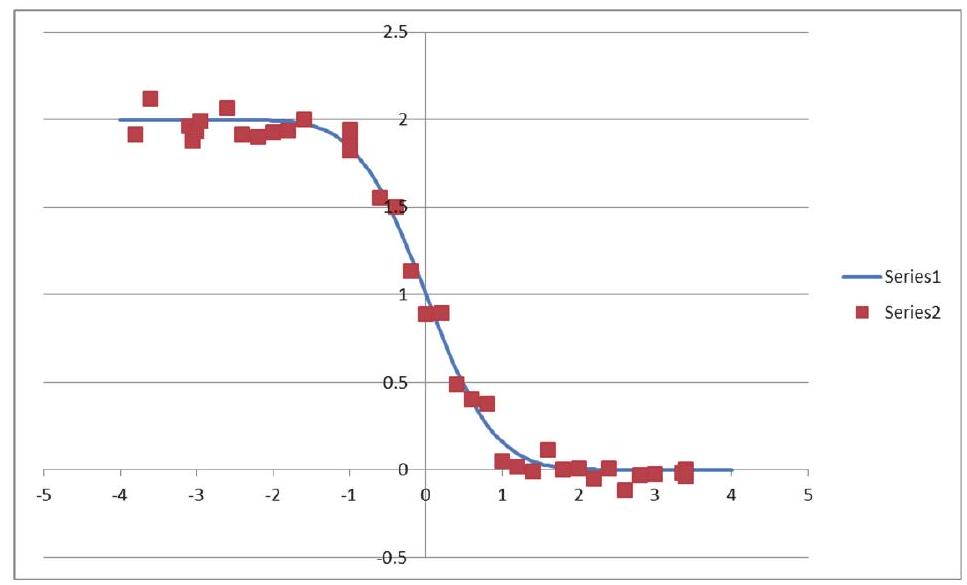
\includegraphics[max width=\textwidth]{2024_04_11_419211c3e451fc7cea07g-028(1)}
\end{center}

(a)

\begin{center}
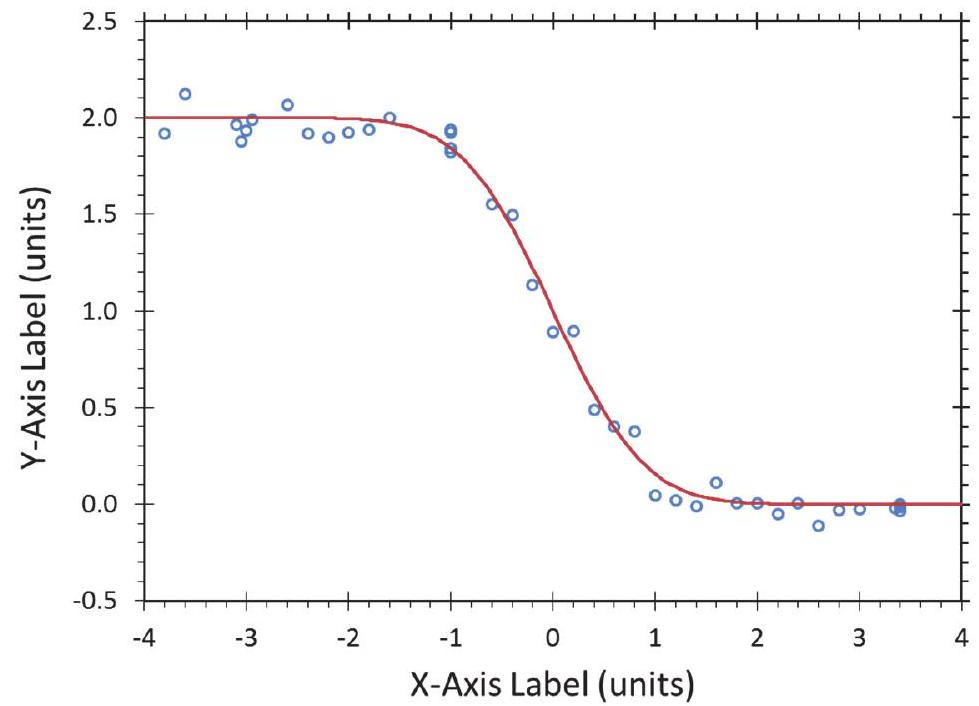
\includegraphics[max width=\textwidth]{2024_04_11_419211c3e451fc7cea07g-028}
\end{center}

(b)

Figure 4.1 Excel graphs of the same data: (a) default scatterplot settings, and (b) after proper formatting. Symbols show data, and the solid line shows the fitted equation.

submission to a scientific journal. My example will be simple: a plot of (made-up) experimental data along with an equation that models that data. The before and after plots are shown in Fig. 4.1.

Here is the sequence of steps I went through in Excel to move from the default (Fig. 4.1(a)) to the final graph (Fig. 4.1(b)). I assumed that the final graph will fit within a single column in a two-page-per-column format. For journals with other page formats, some adjustments to these directions may be required.

\begin{enumerate}
  \item Set the chart area size to be $5 \mathrm{in}$. tall by $6.75 \mathrm{in}$. wide (this is $2 \times$ the final size required by most journals, but it will shrink $50 \%$ when published because most scatterplots will fit in one column). The chart area height can be adjusted as needed, if the data suggest a better shape, but the 4:3 aspect ratio used here is a good default.

  \item Set the chart font size to be 14 points (the size will be $7 \mathrm{pt}$ after shrinking the graph $50 \%$ ).

  \item Remove the legend if not needed (try to put labels inside the graph if they fit rather than using a legend). If using a legend, see if there is room within the plot area to put it. In Fig. 4.1, using the convention of symbols for data and a line for the theoretical equation means that the legend can be embedded in the caption.

  \item Remove all gridlines.

  \item Change the axes' line color from gray (the Excel default) to black and set it to $1 \mathrm{pt}$ thick.

  \item Change the major tick mark to "cross" and minor tick mark to "outside."

  \item Format the chart area to have no border.

  \item Format the plot area to have a solid black border (1 pt thick) and no fill.

  \item Set the "axis crosses" point so that the two axes meet at the lower-left corner.

  \item Adjust the axes' label numbers so that they have the proper number of decimal points.

  \item If necessary, adjust the axes' min and max values (Excel defaults are often poor). Remember that the goal is to use up almost all of the graph space with data, but try to keep the data points from overlapping onto the solid border surrounding the plot area.

  \item Add axis titles, set to $18 \mathrm{pt}$ (less if titles are too long), no bold, and use a rotated vertical title.

  \item Format the "data series" to have the preferred color and symbol or line type/style for maximum readability and differentiation between data series. I typically use a weight of $1.5 \mathrm{pt}$ for my lines, and my preferred symbol is the open circle when more than one thing is being plotted at a time or when data points overlap.

  \item If using line segments to connect data points, never turn on the "smoothed line" feature.

  \item Make sure that there is no title.

  \item Add a baseline in the graph if doing so is helpful for interpreting the data, but do not include a $y=0$ line by default.

  \item Preferred: put tick marks on the right and top of the plot area bounding box (this is tricky to do in Excel; use a "secondary axis").

\end{enumerate}

That is a lot of steps, but every step left out produces a less adequate graph. Note that some of these steps can be described as aesthetic, though making a graph more pleasing to the eye is generally synonymous with making it more readable. For example, the open-circle data symbols enable one to see behind the symbol to the line and to other data points. In the original graph with the solid square symbols, can you tell how many data points are at $x=-1$ and $x=3.4$ ? When using more than one symbol, be sure to consider the symbols' size and shape for maximum visibility when there is overlap.

\subsection*{4.5.2 Other scatterplot examples}
The next example (Fig. 4.2) shows how labels can sometimes be fit into the graph to avoid the need to refer back and forth to a legend.

A regular problem I encounter is a graph with data that fails to use up the space in the plot area. In Fig. 4.3, the authors wish to show the stability of their laser, so they stretch the $y$-axis range to be ten times the data range. As result, we cannot see the variation in the data. So why bother showing the graph? A similar

\begin{center}
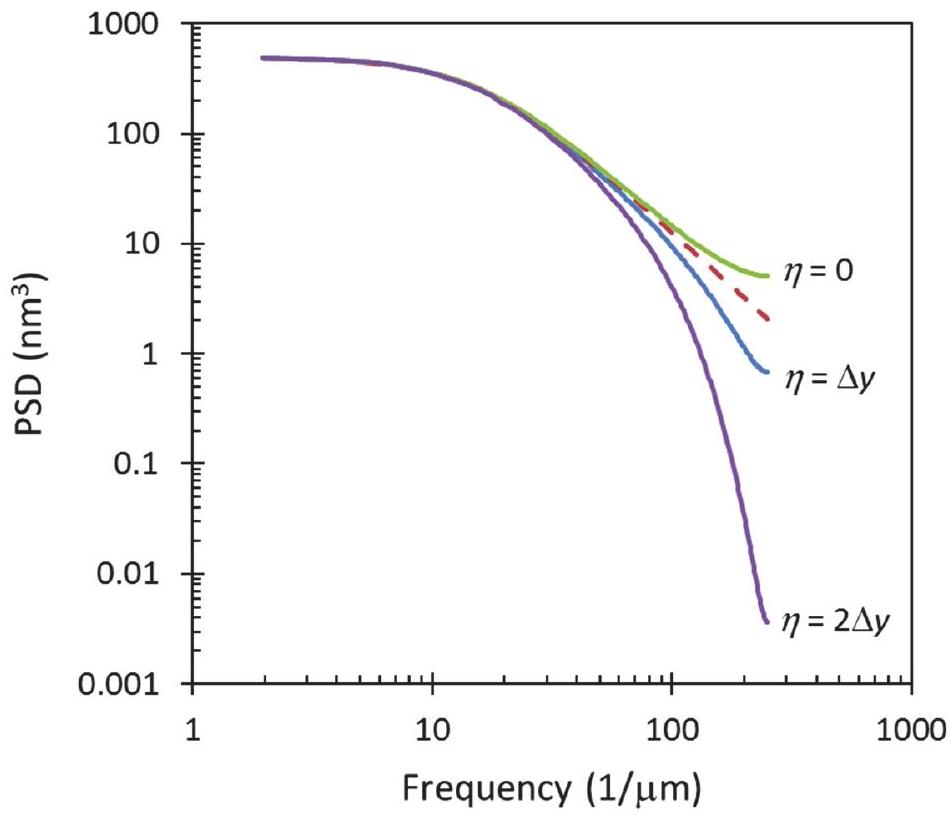
\includegraphics[max width=\textwidth]{2024_04_11_419211c3e451fc7cea07g-030}
\end{center}

Figure 4.2 Labels within the graph avoid the need for a legend. The color used here improves readability online but is not needed for comprehension when printed in black and white. The dotted line is explained as being the reference curve in the figure caption of the original. ${ }^{16}$

\begin{center}
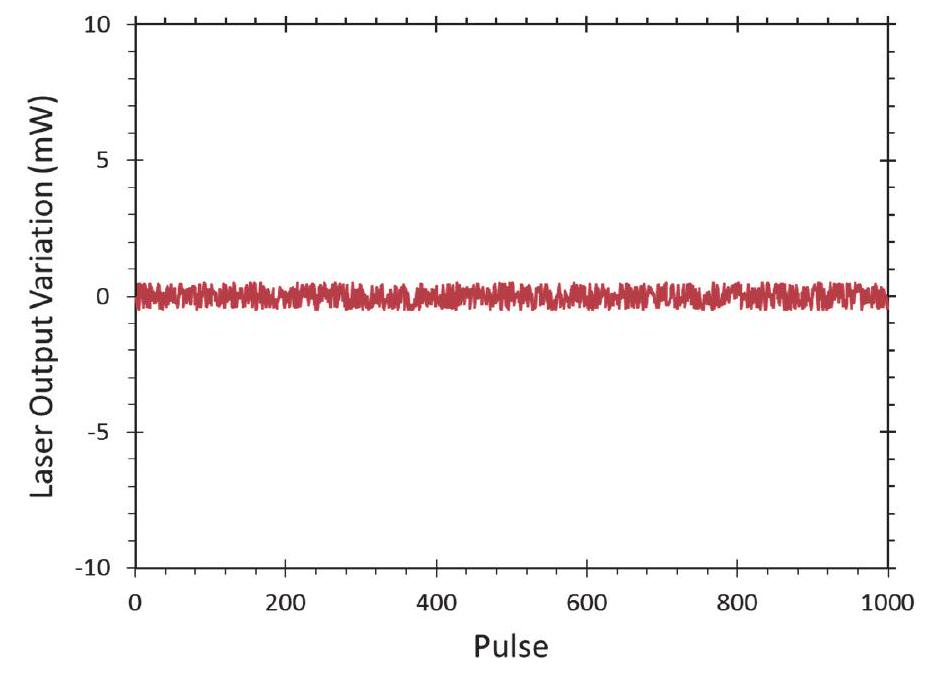
\includegraphics[max width=\textwidth]{2024_04_11_419211c3e451fc7cea07g-031}
\end{center}

Figure 4.3 A wasted graph. The $y$ axis is chosen to give the impression that the there is little variation in the output, but if we cannot see any variation in the data, why show the graph?

effect can be obtained by including zero on the $y$-axis scale even though no data are near zero (imagine a plot of Earth's global surface temperature in Kelvin over time, then starting the $y$ axis at zero-global warming would disappear). This is an example of advocating rather than informing, i.e., using graphs to hide rather than reveal the truth. If there is nothing in the data worth seeing, the graph should be replaced with simple statistics: mean, standard deviation, $\min / \max$ of the output, and maybe a statement that a linear regression gave a slope that was not statistically different from zero. If there is something worth seeing in the data, then adjust the $y$-axis scale so that it can be seen.

There are other ways to mislead with an $x-y$ scatterplot, some not as subtle as the previous example. Unitless axes are a favorite of those who, at a minimum, do not wish to reveal the whole truth. An axis with ambiguous labeling should never be allowed. Using "arbitrary units" for a $y$-axis is a bit trickier because there are some cases where such a label is appropriate (a relative measure, based on a local uncalibrated standard that can be used to compare similar measurements). A common example is the relative intensity used in spectral analysis. Arbitrary units are never preferred but sometimes necessary. Arbitrary units should never be used to hide known units that the author does not want to reveal. Additionally, arbitrary units have an arbitrary scale but not an arbitrary zero point. Thus, when arbitrary units are used the graph must mark the zero point on the scale. One solution is to use a relative scale rather than arbitrary units, with the original clearly defined.

One common and important application of the $x-y$ scatterplot compares different graphs (thus adding a third variable, sometimes more). Figure 4.4 shows a $2 \times 3$ array of graph multiples, matching the $x$-axis and $y$-axis scales to allow easy comparison. With small multiples, many more graphs can be compared.

\begin{center}
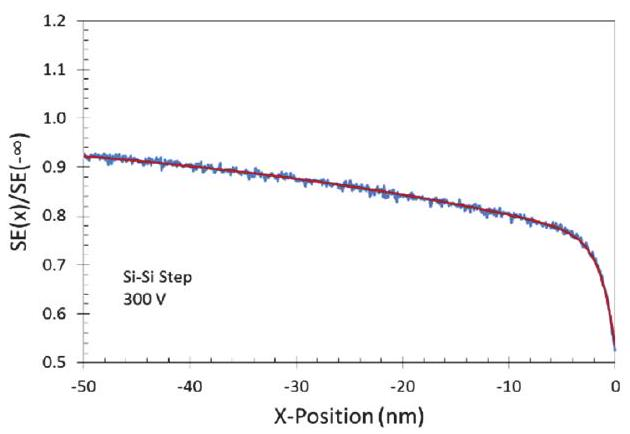
\includegraphics[max width=\textwidth]{2024_04_11_419211c3e451fc7cea07g-032(1)}
\end{center}

(a)

\begin{center}
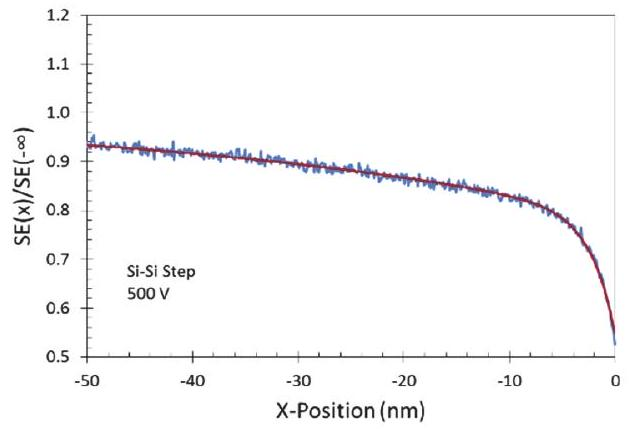
\includegraphics[max width=\textwidth]{2024_04_11_419211c3e451fc7cea07g-032(3)}
\end{center}

(c)

\begin{center}
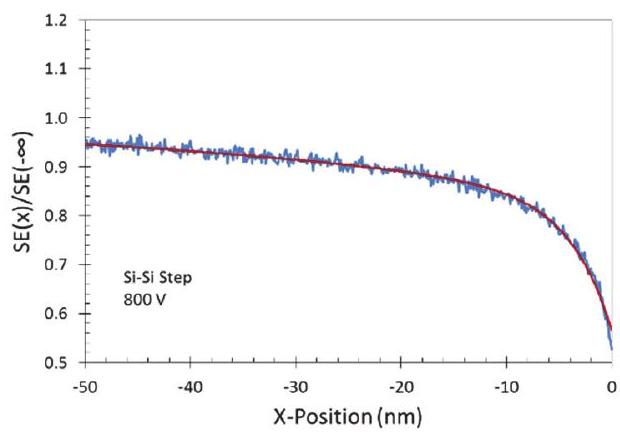
\includegraphics[max width=\textwidth]{2024_04_11_419211c3e451fc7cea07g-032(2)}
\end{center}

(e)

\begin{center}
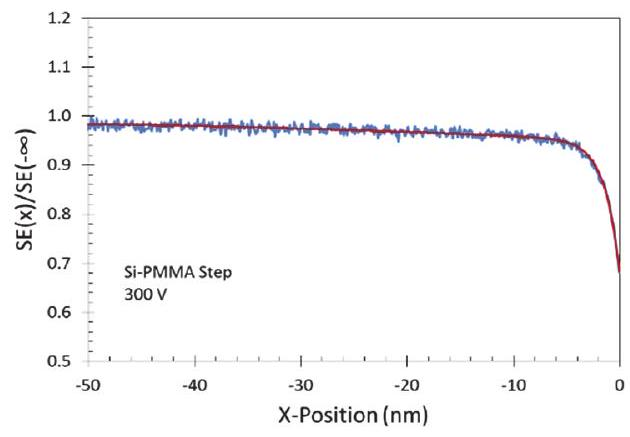
\includegraphics[max width=\textwidth]{2024_04_11_419211c3e451fc7cea07g-032(4)}
\end{center}

(b)

\begin{center}
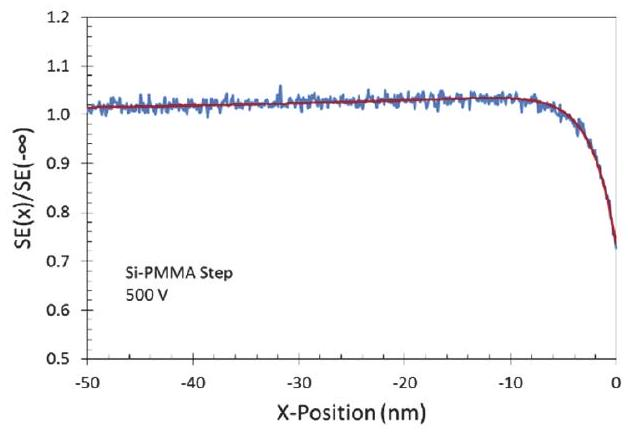
\includegraphics[max width=\textwidth]{2024_04_11_419211c3e451fc7cea07g-032(5)}
\end{center}

(d)

\begin{center}
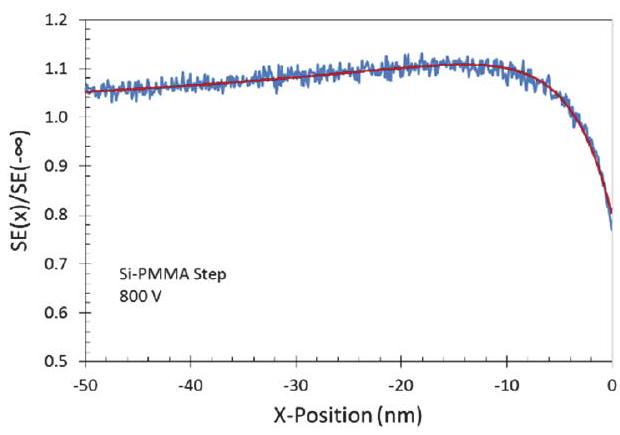
\includegraphics[max width=\textwidth]{2024_04_11_419211c3e451fc7cea07g-032}
\end{center}

(f)

Figure 4.4 Comparison of Monte Carlo simulations to an analytical model. ${ }^{17}$ The smooth (red) line is the equation and the jagged (blue) line is the Monte Carlo simulation results. Both vertical and horizontal comparisons between graphs are enabled by matching the $x$-axis and $y$-axis scales of every graph. Note that in this case redundant axes labels could be removed.

\subsection*{4.6 Figure Quality from a Production Standpoint}
The final step in ensuring a good quality figure in your published paper is to make sure that the submitted figure matches the production requirements of the journal. (I speak here specifically about $\mathrm{JM}^{3}$ requirements, but I do not think they are much different from most other journals.) A few of the largest publications, such as Nature or Science, employ professional editors who can reset a graph to the standards of the journal. For most publications, however, it is up to the author to get the graph right. Below are some hints, given to me by the SPIE publications staff, that will make the production process go more smoothly and produce higherquality graphs:

\begin{itemize}
  \item Submit high-resolution figures. The quality of the published figure is only as good as the original file - it cannot be improved by the typesetter. A resolution of $100 \mathrm{dpi}$ (dots per inch) looks great on a computer screen but is inadequate for print. A minimum of $300 \mathrm{dpi}$ is required, but $600 \mathrm{dpi}$ is preferred. Thus, a one-column wide photograph must be at least 1000 pixels across.
  \item Submit full-size figures (7 in. wide), but remember that they will, in general, be reduced $50 \%$ to fit within one column. Make sure that the fonts, lines, and other elements of the graph will hold up to this reduction (see my font-size suggestions in the earlier Excel example). Try shrinking the graph 50\% and printing it out yourself as a test.
  \item High-contrast color graphics are great for online viewing, but the figures still need to be readable in grayscale for black-and-white printing (unless you pay for color printing). Colors such as red and blue, which are easy to distinguish online, are the same shade of gray when printed in black and white. If lines or symbols must be distinguished in a legend or caption, use different line styles and symbols instead of relying solely on color.
  \item Do not submit JPG files - the image compression often compromises the quality of the figure. TIF files have no compression, but if the file size is unmanageable try using "LZW" compression.
  \item If a figure contains multiple parts (such as Fig. 4.4), they should all be laid out in one file, not submitted as individual files. This is important because it lets the author determine how a figure should be arranged for the reader (horizontal versus vertical, for example). The parts should be clearly labeled with lowercase Roman text in parentheses, i.e., (a), (b), etc.
\end{itemize}

\subsection*{4.7 Tables}
Tables present data directly and are preferred over graphs when the exact numerical values of the data are needed. Still, tables often have a goal similar to that for figures: enabling comparisons. When presenting data in two or more dimensions, the layout and order of the table entries can make a huge difference in the ability of the reader to make the proper comparisons and see the important trends. It is easier for a reader to compare numbers arranged within a row than within a column. It is also easier to compare numbers that are close to each other (preferably next to each other).

Often, 2D tables will benefit from marginal analysis, where rows and columns are totaled or expressed as a percentage of the total. The table in the next section shows an example of such marginal statistics.

As with figures, tables should be made comprehensible on their own, without reference to the text of the paper, if possible. This means that a table should have a good caption, and the items presented should be clearly defined within the table. Do not forget units and uncertainty estimates.

Different journals have different formatting requirements for tables. For example, many journals allow only horizontal lines in the table. Before submitting your manuscript, review the table formatting guidelines (or just look through the journal for examples of tables) and render your table in that format. A table arranged to look good in your preferred style may not work so well in the journals' required style.

\subsection*{4.8 Example: Figures and Tables in $\mathrm{JM}^{3}$}
How are graphs used in my journal, $\mathrm{JM}^{3}$ ? Table 4.1 shows my counts of figures and tables found in the 2012 issues of $\mathrm{JM}^{3}$. The graph types I used are somewhat arbitrary (as all categories are), but hopefully useful. $\mathrm{JM}^{3}$ papers in $2012 \mathrm{had}$ an average of 19 figures and one table per paper, attesting to the importance of figures in our field. About $20 \%$ of the figures were used to explain the theory or experimental setup, and the rest showed results. By far the most common figure was the ubiquitous $x-y$ plot, accounting for $1 / 3$ of all figures and tables. Results micrographs (optical and scanning electron micrographs, as well as atomic force microscope renderings) made up $25 \%$ of the figures. Contour and 3D plots were used about $10 \%$ of the time, with other types of charts filling in the remainder.

While I made no attempt to rate or judge the quality of the figures, it was clear to me from my survey that there were many excellent examples of figures and tables in all categories. There were some poor ones as well.

As an exercise, I rendered the data from the "Results" figures of Table 4.1 into a variety of bar charts (see Fig. 4.5). Most of them fail the test of staying "on message." The first four draw attention to the variations between issues, either in actual numbers or in percentages, though the per-issue variation is not important to my story here. The last two correctly keep the emphasis on the relative frequency of each figure type, with the horizontal bar chart being far more

Table 4.1 Figure and table counts for $\mathrm{JM}^{3}$ papers published in 2012.

\begin{center}
\begin{tabular}{rrrrrrr}
 & Issue \#1 & Issue \#2 & Issue \#3 & Issue \#4 & Total & \% of Total \\
\begin{tabular}{r}
No. Papers \\
Methods \\
\end{tabular} & 24 & 43 & 22 & 12 & 101 &  \\
Photos &  &  &  &  &  &  \\
Diagrams & 92 & 120 & 85 & 25 & 322 & $\mathbf{1 6 . 3 \%}$ \\
Tables & 6 & 11 & 4 & 12 & 33 & $\mathbf{1 . 7 \%}$ \\
\cline{ 2 - 7 }
Setup Total & 109 & 187 & 96 & 40 & 432 & $\mathbf{2 1 . 9 \%}$ \\
Results &  &  &  &  &  &  \\
x-y Plots & 138 & 281 & 120 & 114 & 653 & $\mathbf{3 3 . 1 \%}$ \\
Contour Plots & 47 & 52 & 25 & 62 & 186 & $\mathbf{9 . 4 \%}$ \\
3D Plots & 2 & 10 & 17 & 13 & 42 & $\mathbf{2 . 1 \%}$ \\
Micrographs & 89 & 131 & 222 & 40 & 482 & $\mathbf{2 4 . 4 \%}$ \\
Histograms & 6 & 6 & 4 & 0 & 16 & $\mathbf{0 . 8 \%}$ \\
Bar Charts & 10 & 2 & 4 & 11 & 27 & $\mathbf{1 . 4 \%}$ \\
Wafer Maps & 6 & 0 & 1 & 1 & 8 & $\mathbf{0 . 4 \%}$ \\
Tables & 25 & 53 & 23 & 10 & 111 & $\mathbf{5 . 6 \%}$ \\
Other & 6 & 4 & 3 & 4 & 17 & $\mathbf{0 . 9 \%}$ \\
\cline{ 2 - 7 }
Results Total & 329 & 539 & 419 & 255 & 1542 & $\mathbf{7 8 . 1 \%}$ \\
\cline{ 2 - 7 }
\end{tabular}
\end{center}

\begin{center}
\begin{tabular}{rrrrrr}
\begin{tabular}{r}
Tables and \\
Figures Total \\
Tables and \\
\end{tabular} & 438 & 726 & 515 & 295 & 1974 \\
\begin{tabular}{r}
Figures/Pape \\
\end{tabular} &  &  &  &  &  \\
$\mathbf{r}$ & $\mathbf{1 8 . 3}$ & $\mathbf{1 6 . 9}$ & $\mathbf{2 3 . 4}$ & $\mathbf{2 4 . 6}$ & $\mathbf{1 9 . 5}$ \\
\end{tabular}
\end{center}

aesthetically pleasing. But then, they do not do a better job of conveying the message compared to the table, and the table is far richer and denser in information (and has the added benefit of documenting the data better). This conclusion is quite frequently true of bar charts: a table would be better.

\subsection*{4.9 Conclusions}
When presenting results, a good graph is like a good scientific theory: once you see it, everything just makes sense. But arriving at such a point takes care and consideration. Keeping in mind the advice from this chapter will, I hope, lead to graphs that help you, the author, achieve your goal of effective and efficient communication.
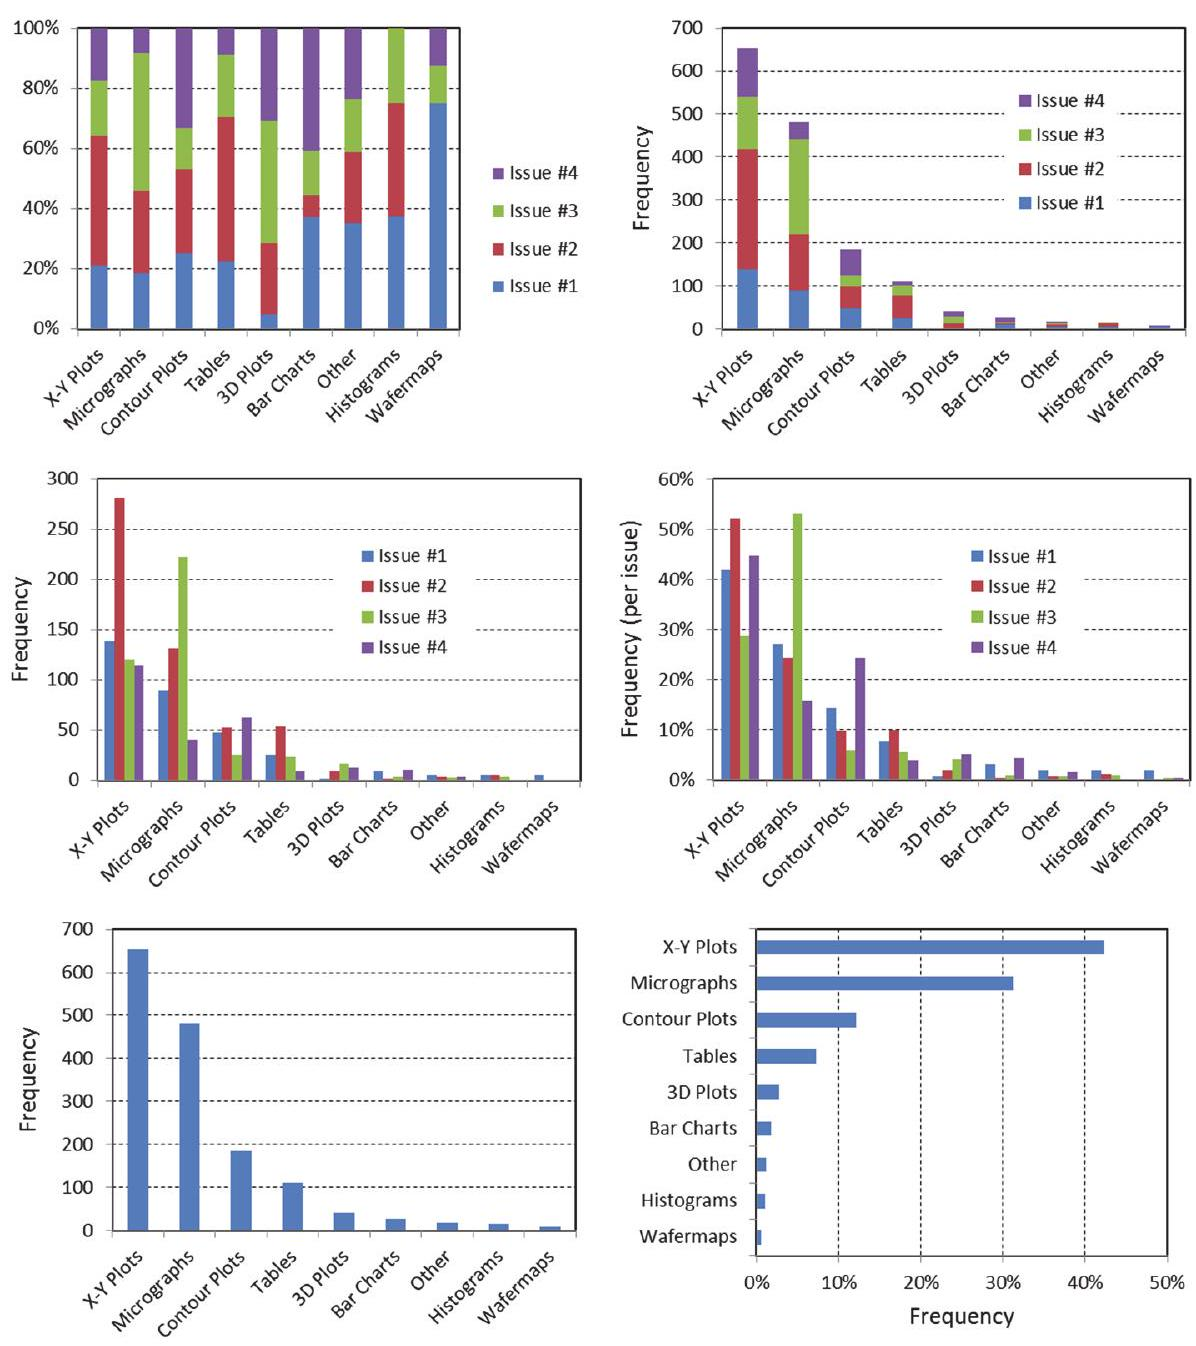
\includegraphics[max width=\textwidth, center]{2024_04_11_419211c3e451fc7cea07g-036}

Figure 4.5 A comparison of six different bar charts based on the data from the "Results" section of the table. The top four graphs are "off-message," emphasizing the per-issue variation. The bottom two have the proper emphasis but are not very data-dense.

They say a picture is worth a thousand words. In a scientific journal, each figure occupies the space of anywhere from 150 to 500 words. So at the very least, a figure should convey more information than the words it displaces. Otherwise, valuable space has been wasted. A good graph can certainly do that, though not all figures do. As the abstract artist Ad Reinhardt so aptly put it, "As for a picture, if it isn't worth a thousand words, the hell with it."

\section*{References}
${ }^{1}$ E. R. Tufte, The Visual Display of Quantitative Information, Graphics Press, Cheshire, CT, p. 6 (1983).

${ }^{2}$ J. W. Tukey, Exploratory Data Analysis, Addison-Wesley, Reading, MA (1977).

${ }^{3}$ W. S. Cleveland, "Graphs in Scientific Publications", The American Statistician 38(4), 261-269 (Nov. 1984).

${ }^{4}$ E. R. Tufte, Visual Explanations, Graphics Press, Cheshire, CT, p. 43 (1997).

${ }^{5}$ M. Kozak, "Basic principles of graphing data", Sci. Agric. 67(4), 483-494 (July/August 2010).

${ }^{6}$ E. R. Tufte, Visual Explanations, Graphics Press, Cheshire, CT, p. 53 (1997).

${ }^{7}$ ibid., p. 70.

${ }^{8}$ W. S. Cleveland, The Elements of Graphing Data, Wadsworth \& Brooks/Cole, Pacific Grove, CA (1985).

${ }^{9}$ E. R. Tufte, The Visual Display of Quantitative Information, Graphics Press, Cheshire, CT, p. 77 (1983).

${ }^{10}$ ibid., p. 168.

${ }^{11}$ W. S. Cleveland, The Elements of Graphing Data, Wadsworth \& Brooks/Cole, Pacific Grove, CA, p. 57 (1985).

12 J. W. Tukey, Exploratory Data Analysis, Addison-Wesley, Reading, MA (1977).

${ }^{13}$ M. Friendly and D. Denis, "The Early Origins and Development of the Scatterplot", $J$. History Behavioral Sci. 41(2), 103-130 (Spring 2005).

${ }^{14}$ J. F. W. Herschel, "On the investigation of the orbits of revolving double stars", Memoirs Royal Astronomical Soc. 5, 171-222 (1833).

${ }^{15}$ The Oxford English Dictionary, $2^{\text{nd }}$ ed., Oxford Univ. Press (1989).

${ }^{16}$ C. A. Mack, "Systematic Errors in the Measurement of Power Spectral Density", $J$. Micro/Nanolithography, MEMS, and MOEMS 12(3), 033016 (Jul-Sep, 2013).

${ }^{17}$ B. D. Bunday and C. A. Mack, "Influence of Metrology Error in Measurement of Line Edge Roughness Power Spectral Density”, Proc. SPIE 9050, 90500G (2014).

\section*{Chapter 5}
\section*{Citations}
As described in the Preface, the growth of scientific knowledge is predominately incremental - we build on past knowledge more often than we displace it. Thus, the first pillar of science-a communal collection of knowledge-requires mechanisms for preserving and disseminating knowledge within the scientific community. By far the most important mechanism in use today is the scientific publication. Although there are many forms of scientific publication, the two most common are the conference presentation (with or without some non-peer-reviewed written text) and the peer-reviewed journal paper (both in print and online).

Because virtually all scientific advances build on past knowledge, it is critical that the new work be placed in the proper context with respect to the past work upon which it builds. The primary mechanism for this is the citation (or reference). Within a scientific paper, references are placed to other works, creating points of contact with the communal collection of scientific literature in order to fit the new work into the web of knowledge. But given the skeptical attitude that is also a part of science, citations are also used to help readers verify the quality of the new work and assess the strength of its conclusions.

\subsection*{5.1 The Five Goals of Citations}
A citation is, by definition, a reference to a source of information or data. Things that can be cited include journal articles, conference proceedings, books, student theses, newspapers, non-print sources (such as film or other recorded media), websites or other online resources, computer materials (such as a published CDROM of data or a piece of software), and personal communications. The citation should be located in the text in such a way that it is clear what material requires the citation. Often, this is at the end of a sentence, but sometimes it must be put in the middle of the sentence to enhance clarity. Obviously, citations must supply sufficient detail so that the referenced material can be found and uniquely identified. As such, every journal establishes a specific format for citations that must be followed. (Alas, there is no universal format that all journals follow.)

Though simple in concept, citations in a scientific paper serve many goals. The five most important goals are

\begin{itemize}
  \item Provide sufficient context of the work to allow for critical analysis of the work by others and thus to enable the readers to gauge for themselves whether the author's conclusions are justified;
  \item Give the reader sources of background and related material so that the current work can be understood by the target audience (thus creating a web of science);
  \item Establish credibility with the reader (e.g., the authors knows the field, have done their homework, etc.) and/or inform the reader that the paper belongs within a specific school of thought;
  \item Provide examples of alternate ideas, data, or conclusions to compare and contrast with this work; and
  \item Acknowledge and give credit to sources relied upon for this work (i.e., acknowledge the use of another's ideas or data), thus upholding intellectual honesty.
\end{itemize}

Of these five goals, the most commonly mentioned is to give credit to others (the so-called normative theory of citations ${ }^{1}$ ) and thus demarcate what credit is due the new work. In truth, scientists can have big egos. We are frequently motivated by the desire for peer recognition. Thus, we try to carefully stake a claim to new ideas or data in our paper, knowing full well that others will be checking to make sure we do not claim too much. Even so, there is no pretense that a list of references will provide a complete list of influences; such a list would be excessive in even the simplest of cases.

While important, the "give credit" purpose of citations is, in my opinion, less compelling than the other goals. I view citations, like all aspects of scientific writing, from a simple perspective: what best serves the needs of the reader? Thus, the primary goal of citations should be to help the reader gain the most from the paper. Imagine your paper being read by graduate students or postdocs: smart, but new to the field. If they read all of the citations, will they have enough background to understand your work? Will any of the references be unneeded or redundant (and thus a waste of the reader's time)? Chances are very good that a simple test will be sufficient to decide on most references: will adding this reference here make the paper more valuable to the reader, or less?

\subsection*{5.2 The Literature Search}
A new research project almost always begins with a literature search, as discussed in Chapter 1. Thus, you should have a good idea what the key papers in the field are before you begin the research. This literature search should be updated during your research, especially as new ideas come or directions change. A review of your literature search results just before you begin drafting your manuscript will allow you to cite as you write. Also, other researchers are often working on similar topics and may have published papers after your original literature search was completed.

A common mistake is to save the literature search until the end of the paper writing process. Doing a literature search only at the end often generates spurious citations (a problem that will be discussed in Section 5.4) and rarely provides the most valuable citations.

\subsection*{5.3 Verify, Verify, Verify}
One of the most pervasive problems with citations is that they are frequently incomplete or inaccurate. It is the job of the authors to verify the accuracy of the references. Editors, copyeditors, and reviewers are not responsible for reference accuracy and are not expected to check references for accuracy. And though copyeditors try to flag incomplete or improperly formatted references, it is the authors who must ultimately fix the errors found. Why not do the work up front to ensure that the references are complete, accurate, and properly formatted? It will only save time and effort in the end, and indicate to the editors and reviewers that you care enough to pay attention to these important details.

Alas, far too few authors take this advice seriously. Several studies have found that between 34 and $67 \%$ of references in a variety of medical and biomedical journals contained errors. ${ }^{2}$ These errors can be broken down into major and minor errors. A major error means that the article could not be found given the information in the citation. One study found that major errors occur in $7 \%$ of the citations from one class of medical journals. ${ }^{3}$ Minor errors include punctuation or spelling mistakes, mistakes in the article titles, mistakes in the name and initials of the author(s), and citation style mistakes. These errors serve as irritants to the reader-they can still find the article, but they have to put more effort into it.

It is probably obvious that the main cause of errors in citations is simple sloppiness on the part of the author. There is another problem, however, that may also be at work: copying citations from other papers. In other words, some authors commit a cardinal sin of citations and add a reference without ever having read that paper. Copying citations from other papers without actually looking up and reading that paper can result in a propagation of errors that are never corrected ${ }^{4}$ (like a children's game of "telephone"). A slightly less egregious form is the abstract citation: citing a paper after reading only the abstract. Both types of unread citation should be avoided: cite only papers you have read.

\subsection*{5.4 Other Problems with Citations}
There are other reasons why a specific reference does not fulfill the goals set out here and thus does not benefit the reader.

Spurious citations: citations that are not needed but are included anyway. These citations are sometimes added at the last minute, after the paper is written, to give the impression that a literature search and proper citation work have been done. They often include redundant citations, where the extra citations do not add any value beyond the first one. A simple example was given by Brian Thompson: ${ }^{5}$ "related work on the technique has been carried out by numerous researchers. ${ }^{1-101 \text{ ", }}$ The problem is obvious: an interested reader must wade through far too muc literature to get the needed background. Sometimes spurious cites are meant to give an impression of erudition by citing an obscure, historical reference (if the referenced work is in a foreign language, all the better).$^{6}$ In all such cases, simply asking the question "If the reader looks up this reference, will it be time well spent?" will be enough to decide if that reference is spurious.

Biased citations: references added (or omitted) for reasons other than meeting the five goals of citations. Biases include overciting of friends' or colleagues' work, omitting cites to the work of rivals, and gratuitous citations in an attempt to curry favor with a boss or potential referee.

Self-cites: citations to one's own work. There is nothing wrong with selfcitations, per se. After all, the work represented in a single paper is often just the latest result of a larger ongoing project. As such, citations to one's earlier work are often perfectly appropriate and sometimes required. Self-cites are a problem when they are either spurious or biased. ${ }^{7}$ Knowing as we do the tendencies of many scientists toward self-promotion, one fears that self-cites may be designed to boost the recognition of the author rather than increase the value of the paper to the reader.

Excluding contrary evidence: a form of biased citations where citations to prior work whose conclusions or data contradict the current work are omitted. Because one of the five goals of citations is to explicitly contrast the new work with prior work containing conflicting data or conclusions, avoiding such conflict (for whatever reason) does not serve the interest of science.

In the end, authors must find a balance between too many and too few citations. The literature base even on vary narrow topics is often vast, and it can be difficult to pick a small subset to cite. In general, authors can mitigate citation problems by asking two questions:

"Have I provided the references that will make this paper as useful as possible?" "If the reader looks up a given reference, will it be time well spent?"

\subsection*{5.5 More on Self-Citations}
Citations sometimes have significance for reasons other than the five listed above. Citations can be counted, and in a data-driven world these counts have assumed outsized importance as a proxy for the influence of a given paper. Citation counts serve as (flawed) measures of journal importance (the impact factor) and researcher clout (the h-index, among other metrics). Today, such citation counts and their metrification are used in hiring and promotion decisions, especially in academia, often as a substitute for thoughtful and informed judgment.

Be careful what you measure, because a truism of the business world is 'what gets measured gets managed'. And measures that come with rewards often get gamed. When a person's career or reputation depends on citation counts, the temptation to inflate those counts is never far away. Some authors are more likely to cite their colleagues' work than their competitors'; some journals expect their submitting authors to preferentially cite work published in that journal. But th easiest way to promote your own work (and thus yourself) is with the self-citation: a citation to one's own prior work.

Self-cites are not inherently problematic. Most scientific publications describe a part of a longer-term research effort, and self-citations can put the new publication in the context of that larger effort. Self-cites become a problem only when they are either spurious or biased. Because deciding that a specific citation is either spurious or biased requires a judgement based on the cited work, the paper in which the citation occurs, and the field within which the work resides, it is not always an easy evaluation to make. Some cases are obvious, as when a majority of a research paper's citations are to the author's own work in a popular field of research. Other cases are less obvious, as when the authors are nearly the only ones working on a very specialized topic. Still, I think most authors know when they are pushing into spurious or biased territory with their self-citations. So the best defense against abuse is self-regulation.

Or is it? An interesting study commissioned by the Chronicle of Higher Education looked at the role of gender in self-citation rates. ${ }^{8}$ An examination of 1.7 million $J S T O R$ papers spanning disciplines and over 60 years found that nearly $10 \%$ of citations were self-citations. Further analysis showed that men were $56 \%$ more likely to cite their own work than women, with the gender disparity growing over time. Apparently, self-regulation of self-citations is more effective in women than men.

What is the cause of this gender disparity? Women in academia seem less inclined to self-promotion than men, probably to their detriment. Does society pressure women to be more "feminine" and modest about their accomplishments? Are men encouraged to be more aggressive in pursuit of career success? Do women work on smaller teams with fewer publications and fewer opportunities for selfcitations? I am certainly not qualified to address such heady questions, but regardless of cause the issue of gender disparity in self-citations has consequences.

In the age of Big Data, success breeds success, and popularity snowballs. The most linked webpages, the most watched videos, and the most downloaded journal papers are "recommended" or promoted to website visitors and social media consumers, generating a handful of winners-take-all and a long tail of neglected also-rans. The bandwagon effect seems true in the world of academic citations as well. Could it be that even modest differences in self-citation rates might snowball into noticeable differences in total citations? In other words, does self-promotion through self-citation work?

One 2007 study showed that it does, with each self-citation multiplying into three other citations to that author over a five-year period. ${ }^{9}$ Further, the penalties for excessive self-citation seem to be small or none. Although this study looked at papers published from 1981-2000, I imagine that the higher levels of online searching and reading today have only increased this multiplying effect. Differences in self-citation rates are likely only one of many factors contributing to gender disparities in academic careers, but it may be one of the easier ones to address.

Proper citations require careful consideration of the appropriate goals of citations, aided by a simple ethos: make the paper reader-centric, not authorcentric. Self-promotion is an author-centered way of looking at the activity of publishing, and it is neither good nor bad when considering the needs of the reader. Though self-cites should not be added to a paper solely for self-promotion, neither should self-cites be avoided for fear that they might appear self-promoting and thus unseemly. By focusing on the reader and the five proper goals of citations, most problems concerning citations can be easily avoided.

\subsection*{5.6 Conclusions}
To do a good job of providing citations in a scientific publication, one must keep in mind the multiple goals of proper citing. But like other aspects of good scientific writing, a simple theme has emerged: make the paper reader-centric, not authorcentric. Although it is common to choose citations that make the paper more valuable to the author (by demarcating what is novel, for example), good citations make the paper more valuable to the reader. Unfortunately, doing a good job of citing requires more work from the authors. But careful citing is worth the effort if your goal is a quality scientific publication.

\section*{References}
\footnotetext{${ }^{1}$ M. H. MacRoberts and B. R. MacRoberts, "Problems of Citation Analysis: A Critical Review", J. Am. Soc. Inform. Sci. 40(5), 342-349, (1989).

${ }^{2}$ M. Wright and J. S. Armstrong, "The Ombudsman: Verification of Citations: Fawlty Towers of Knowledge?”, Interfaces 38(2) 125-139 (2008).

${ }^{3}$ A. E. Mohammad and D. M. Laskin, "Citation Accuracy in the Oral and Maxillofacial Surgery Literature”, J. Oral Maxillofac. Surg. 66(1), 3-6 (2008).

${ }^{4}$ M. V. Simkin and V. P. Roychowdhury, "Read before you cite!", Complex Systems 14(3), 269-274 (2003).

${ }^{5}$ B. J. Thompson, “What is a Reference?", Opt. Eng. 34(7), 1861 (1995).

${ }^{6}$ A. Lakhtakia, "Editorial: False Erudition", J. Nanophoton. 3, 039902 (2009).

${ }^{7}$ J. Hartley, "To cite or not to cite: author self-citations and the impact factor", Scientometrics 92(2), 313-317 (2012).

${ }^{8}$ R. Wilson, "Lowered Cites", The Chronicle of Higher Education 60(27), \href{http://chronicle.com/article/New-Gender-Gap-in-Scholarship/145311}{http://chronicle.com/article/New-Gender-Gap-in-Scholarship/145311} Accessed 7/2/2015 (March 17, 2015).

9 J. H. Fowler and D. W. Aksnes, "Does self-citation pay?", Scientometrics 72(3), 427437 (2007).
}
\section*{Chapter 6}
\section*{Abstract and Title}
In the era of online searches and digital libraries, the importance of a good title and abstract in a scientific paper is perhaps obvious. Yet, bad titles and poorly written abstracts are exceedingly common in the scientific and technical literature. In this chapter, I will talk about some of the common mistakes made in paper titles and abstracts, and then describe a nearly foolproof approach to writing good ones. The result will be a manuscript that is more likely to be accepted by a peer-reviewed journal and a paper that is more likely to be discovered and read by the people who should.

The purpose of a title and abstract is often described as "selling" the paper: getting someone reading the title to read the abstract, and someone reading the abstract to go further and read the paper. ${ }^{1,2}$ I have a different viewpoint. The true purpose of the title and abstract is to get the right people to read your paper. More than $99.9 \%$ of the scientific papers published each year are papers that I have no need and no desire to read. But there are a few papers that I should not miss - and those papers are different for me than for other readers. Thus, the purpose of the title and abstract is matchmaking: matching a paper with the right readers, i.e., those who want and need the information contained in the paper. As the $19^{\text{th }}$ century English writer and eccentric Charles Caleb Colton said, "That writer does the most who gives his reader the most information and takes from him the least time." Nothing works better than a well-written title and abstract to make sure that the wrong reader does not waste time on the wrong paper, and that the right reader does not mistakenly skip over the right paper.

The title (followed by the abstract) is the first thing a reader sees, and so it should be the last thing an author writes (just after the abstract). Because the abstract should be written before the title, I will talk about abstracts first.

\subsection*{6.1 Writing an Abstract}
The most common mistake in writing an abstract is to not pay much attention to it. Authors sometimes consider the abstract as an afterthought, something that can be thrown together after the "real" manuscript is written. I have even seen abstracts that are nothing more than the first paragraph of the introduction. Needless to say such a poor abstract is unlikely to encourage a potential reader (or a journal editor) to venture further.

The abstract should be a concise, stand-alone summary of the paper that covers the following topics: ${ }^{3}$

\begin{itemize}
  \item Background/motivation/context,
  \item Aim/objective(s)/problem statement,
  \item Approach/method(s)/procedure(s)/materials,
  \item Results, and
  \item Conclusion(s)/implications.
\end{itemize}

(You may have noticed that these topics are the typical headings of the major sections of the paper itself, as discussed in Chapter 2. This is not a coincidence.) A typical abstract is about 150-200 words (although maximum allowed lengths vary depending on the journal and paper type), so every word must be chosen carefully. "Concise and precise" is a common maxim. If any one of these five components is missing from the abstract, there is the chance of making a poor match between reader and paper. If the abstract is too wordy, readers may give up before finding what the paper is about.

Although I will describe my preferred approach to the abstract in a moment, let me start by mentioning a common alternative: the newspaper lede. ${ }^{4}$ It is conventional wisdom in the newspaper world that if you do not capture the attention of readers in the first sentence or two, they will move on to another article. Thus, the lead paragraph begins with a sentence that contains the main point of the piece. The second sentence contains the second most important point, etc. By the time the first paragraph is finished, the classic "who, what, where, when, and why" questions have all been answered.

This newspaper lede approach can be used in the scientific abstract as well: if I have only one sentence to convince the reader to continue reading, what would I say? Then ask the same question for each succeeding sentence. There are certainly some good abstracts that have been written using this approach, but I do not like it for two reasons. First, it takes a very good writer to make the newspaper lede form of abstract work. And most of us are not good enough writers to make it work. It is also easy to leave out one of the important five topics that every abstract should contain. Thus, even an extremely well-executed newspaper-lede-style abstract may not do the best job of matchmaking between the paper and the reader. Second, there is a better approach: the structured abstract.

\subsection*{6.2 Structured Abstracts}
For the past 25 years, structured abstracts have become required in most medical journals, though they are not very common in engineering and the physical sciences. ${ }^{5}$ I hope this will change because I am a big fan of the structured abstract. Simply put, the structured abstract formalizes the five topical areas mentioned earlier by adding subheadings and subsections (the "structure") into the abstract.

Although the exact structure can be modified to suit the topics of the journal (or even the specific paper), in engineering and physical sciences a five-structure format is probably best: background, aim, approach, results, and conclusion. Each subsection should contain one to two sentences, answering the following questions:

Background: What issues led to this work? What is the environment that makes this work interesting or important?

Aim: What did you plan to achieve in this work? What gap is being filled? Approach: How did you set about achieving your aims (e.g., experimental method, simulation approach, theoretical approach, combinations of these, etc.)? What did you actually do?

Results: What were the main results of the study (including numbers, if appropriate)?

Conclusions: What were your main conclusions? Why are the results important? Where will they lead?

The benefit of the structured abstract is twofold: it forces the author to include information from all five categories, and it makes these five sections easy to find and access. Although it is logical that structured abstracts will be better than unstructured abstracts, there is also proof that this is so. The preeminent researcher into the efficacy of structured abstracts, James Hartley, reviewed some 31 studies that had been performed by 2004 and found that these studies demonstrated the superiority of structured abstracts. ${ }^{6}$ His review, as well as others, ${ }^{7}$ showed that structured abstracts

\begin{itemize}
  \item contain more information,
  \item are easier to read,
  \item are easier to search,
  \item facilitate peer review, and
  \item are preferred by readers and authors.
\end{itemize}

This is all well and good, but most journals do not use structured abstracts. The structured abstract is still important because it can be used in what I call the structural method of abstract writing. The method is quite simple. First, write a structured abstract. When you are finished and satisfied with the result, simply delete the subheadings and combine all of the lines into one paragraph. Finally, reread this new abstract and change the beginnings of sentences to increase readability and flow, if needed (though this will usually not be necessary). The result will be a well-written and effective abstract with most of the benefits of a structured abstract.

To illustrate, the following is an abstract from one of my papers. First, I wrote a structured abstract:

Background: Photoresist development rate can be defined microscopically (the development rate at a point) or macroscopically (the propagation rate of an average resist height). In the presence of stochastic noise, these two rates will be different.

Aim: In order to properly calibrate lithography simulators, the difference between these two definitions of development rate should be quantified.

Approach: Using theoretical derivations and a stochastic (Monte Carlo) resist simulator, the propagation rate of a resist surface is characterized in the presence of stochastic variation in the resist deprotection concentration and a nonlinear development rate response.

Results: The resulting propagation rate can be more than an order of magnitude higher than for the case of no stochastic noise. Correlation in the development rate creates an effective surface inhibition over a depth into the resist of several correlation lengths.

Conclusions: The differences between microscopic and macroscopic dissolution rate can have an important effect on how development rate models should be calibrated, depending on their use in continuum or stochastic lithography simulators.

Then, after deleting the subheadings and line breaks, a traditional abstract format is obtained. I added a transitional clause at the front of the last sentence to make the abstract flow better, though this small change could easily have been left out:

Photoresist development rate can be defined microscopically (the development rate at a point) or macroscopically (the propagation rate of an average resist height). In the presence of stochastic noise, these two rates will be different. In order to properly calibrate lithography simulators, the difference between these two definitions of development rate should be quantified. Using theoretical derivations and a stochastic (Monte Carlo) resist simulator, the propagation rate of a resist surface is characterized in the presence of stochastic variation in the resist deprotection concentration and a nonlinear development rate response. The resulting propagation rate can be more than an order of magnitude higher than for the case of no stochastic noise. Correlation in the development rate creates an effective surface inhibition over a depth into the resist of several correlation lengths. These results show that the differences between microscopic and macroscopic dissolution rate can have an important effect on how development rate models should be calibrated, depending on their use in continuum or stochastic lithography simulators.

Note that although structured abstracts are typically longer than traditional ones, the 166-word length here is right on target for most journals. If anything, the approach and results sections could have been expanded slightly.

Additionally, the structured method of abstract writing also helps to avoid useless but all-too-common phrases like "in this paper" and "we report" or "will be discussed." The abstract should talk about the work, not about the paper; phrases like "is discussed" turn your abstract into a table of contents rather than a summary of the paper. Do not use the first person ("I" or "we" or "the author"). Also, there is rarely a need to use phrases like "new" or "novel" in the abstract because only the novel results should be mentioned.

\subsection*{6.3 Important Additional Thoughts on Abstracts}
Why should the abstract be written after the entire paper is complete? The reason is simple: if not, it is unlikely that the abstract will be accurate. A study of six highly regarded medical journals in 1999 found that about $40 \%$ of the abstracts studied contained information inconsistent with the body of the paper, or information not found in the body of the paper, or both. ${ }^{8}$ The most likely cause of these errors, after just plain sloppiness, would be changes made to the paper after the abstract was written. Such errors and inconsistencies can largely be avoided by leaving the abstract-writing task until after the body of the manuscript is completely finished. The structured abstract can help make the abstract more informative, but it is still up to the diligence of the authors (and journal editors and reviewers) to make sure the abstract is accurate. There is a three-part test that should be applied to your abstract when you are finished:

\begin{enumerate}
  \item Is all of the information in the abstract consistent with what is written in the body of the paper?

  \item Can all of the information found in the abstract also be found in the body of the paper?

  \item Is the important information of the paper found in the abstract? Are any key words from the paper missing from the abstract?

\end{enumerate}

The abstract must be self-contained, and it should generally not contain citations to other papers. If a citation is required (for example, if the paper is a response to a previous publication), then the full citation must be embedded in the abstract. Avoid abbreviations and acronyms in the abstract, but if you insist on including one, spell it out the first time it is used. Do not refer to figures or tables from the body of the paper, or use words or descriptions that will only make sense after the full paper has been read.

As with all writing, keep the audience in mind. If you are writing a spectroscopy paper for a spectroscopy journal, you can surmise that all of your readers will be spectroscopists, with a certain background knowledge assumed. A paper on that same topic for a more general optics journal may require an extra sentence in the background section of the abstract to inform the reader that the topic is within the field of spectroscopy, within a certain subfield, etc.

Finally, an important goal of the abstract (and the title, to be discussed next) is to make the abstract as specific as possible while still describing the full range o work reported in the body of the paper. If the paper measures only the thickness uniformity of a film, the abstract should not make the more general claim that the paper measures "film uniformity." If the paper simulates the scattering properties of 1D gratings (but not more general objects), an abstract that merely states that scattering simulations were performed could mislead the reader into thinking that the work was applicable to more general objects. On the other hand, if the thickness and compositional uniformity of the film were measured, saying only "thickness uniformity" in the abstract is too limiting and does not describe the full scope of the paper.

\subsection*{6.4 Titles}
Once the abstract is finished, it is time to write the title. Unfortunately, it is against human nature to write the title last. Instead, the title is often the first thing written, at the top of that blank document that will soon become your manuscript. It is important to consider these first words as the working title. When the manuscript, and the abstract, are finished, it will almost surely be necessary to revise the title.

It is probably impossible to define a universal procedure for creating a good title- there is no equivalent "structure method" for writing a title. There are some basic guidelines, however, that make use of the structured abstract to guide the creation of the title. In general, the title should reflect the aim and approach of the work. Depending on the audience (and the specificity of the journal), some of the background may have to be included. Rarely are results and conclusions even hinted at in the title. Let us look at each of these items through the use of an example.

Unlike the worlds of newspaper reporting and marketing press releases, the title of a scientific paper should describe the aim of the work, not the results. Thus, a good title might be

\section*{Impact of temperature and pressure on the compositional uniformity of sputter-deposited aluminum alloys}
The following news-style title, on the other hand, is not appropriate:

\section*{Optimizing temperature and pressure improves sputter-deposited aluminum alloy films}
Note that the good title is essentially a statement of the aim of the work. Often, it is important to mention the approach used as well, though an experimental approach is generally assumed if it is not mentioned. If the study had been based on simulation (or some other approach), however, this would generally be included in the title:

\section*{Impact of temperature and pressure on the simulated compositional uniformity of sputter-deposited aluminum alloys}
The title should be as specific as possible while still describing the full range of the work. For example, if only one aluminum alloy was studied, that specific alloy should be mentioned in the title. If only aluminum alloys are studied, the title shouldn't say "sputter-deposited metals" or "sputter-deposited alloys." On the other hand, the title should not say "aluminum alloys" if gold was also included in the study. If the title had said "uniformity" rather than "compositional uniformity," the reader could easily have believed that the paper was about thickness uniformity or some other parameter. And if only sputter deposition was studied, then leaving this information out would make the title insufficiently specific.

A conflicting goal of the title is to be as short as possible (in 2011, titles in the Journal of Micro/Nanolithography, MEMS, and MOEMS ranged from 4 to 21 words in length, with an average length of 11.5). Specificity can often be improved through the use of more words, but a title that is too lengthy may not be read. ${ }^{9}$ Finding the best compromise between descriptiveness and brevity is where the art of authorship comes into play. Going back to our example, here is a title that sacrifices too much specificity to obtain brevity:

\section*{Impact of process parameters on the uniformity of aluminum alloys}
A good test for your title is to answer these questions: Does the title of your manuscript, seen in isolation, give a full yet concise and specific indication of the work reported? Would someone interested in the exact topic of your paper, reading this title, be inclined to read the abstract?

Avoid being overly clever with the title - a pun or a play on words may be great fun, but it is unlikely to help your article be found by a search engine (and can be easily misunderstood by an international audience). Titles should also be free of jargon unlikely to be understood by those not intimately familiar with the topic, and they should not contain acronyms. The overall goal should be a title that is clear and informative.

\subsection*{6.5 Keywords}
This brings up the next topic-keywords (also called "subject terms"). We are quickly passing out of the days when most people will find your article by flipping through the print version of the journal. Today, your article is unlikely to be widely read unless it comes up relatively high on a general or science-specific searchengine-results list. The first and most important thing you can do to ensure that your article is found by readers looking for it is to do a good job of writing the abstract and title. Following the advice given earlier should help. After that, you must decide on appropriate keywords.

The important idea behind identifying the keywords to be listed under the abstract as "subject terms" is simple: if you were looking for an article on exactly the topic of your manuscript, what words would you type into a search engine in order to find it? Chances are you would start with only two to four words or phrases. If that resulted in too many hits, or too many off-scope articles, then you would refine your search by adding one or two more phrases. These are the word or phrases (plus all of their common variants and synonyms) that should be included in the list of subject terms.

After you have a good list of keywords, go back and look at your title and abstract. Are these keywords found in the title and abstract? If not, someone searching for your article may easily miss it. The most important keywords should be found in the title, and in the abstract several times.

\subsection*{6.6 Conclusions}
A structured abstract is a proven way to give readers the information they need in an accessible and readable format. The structure method of abstract writing described here can provide many of the benefits of a structured abstract for journals that do not use structured abstracts. This structure can also aid in the writing of the title, using information from the aim and approach subsections.

Too often, abstracts (and sometimes even titles) are written as afterthoughts and not given the attention they deserve. The title and abstract are the first and most important way to match potential readers with your paper. Following the advice in this chapter will help to get your paper read by the right people.

\section*{References}
\footnotetext{${ }^{1}$ R. G. Driggers, "Editorial: how do you write a great abstract and why is it important?", Opt. Eng. 49(6), 060101 (2010).

${ }^{2}$ W. Rhodes, "Editorial: the abstract as a marketing tool", Opt. Eng. 49(7), 070101 (2010).

${ }^{3}$ National Information Standards Organization, "Guidelines for abstracts", ANSII/NISO Standard 239.14-1997 (1997).

${ }^{4}$ The neologism "lede" means simply the "lead" (guide or beginning) and is used to distinguish between other meanings (and pronunciations) of that word.

${ }^{5}$ R. N. Kostoff and J. Hartley, "Open letter to technical journal editors regarding structured abstracts: this letter proposes that structured abstracts be required for all technical journal articles", J. Inform. Sci. 28(3), 257-261 (2002).

6 J. Hartley, "Current findings from research on structured abstracts", J. Med. Libr. Assoc. 92(3), 368-371 (2004).

${ }^{7}$ C. Zhang and X. Liu, "Review of James Hartley's research on structured abstracts", $J$. Inform. Sci. 37(6), 570-576 (2011).

${ }^{8}$ R. M. Pitkin, M. A. Branagan, and L. F. Burmeister, "Accuracy of data in abstracts of published research articles”, J. Am. Med. Assoc. 281(12), 1110-1111 (1999).

${ }^{9}$ H. R. Jamali and M. Nikzad, "Article title type and its relation with the number of downloads and citations”, Scientometrics 88, 653-661 (2011).
}
\section*{Chapter 7}
\section*{What an Editor Looks For}
Everyone who submits a manuscript for peer review dreads one thing above all else: getting rejected (though the gentlefolk among us journal editors prefer the phrase "decline to publish"). There are many reasons why a manuscript might be rejected, and a good understanding of the reasons can help you make sure your manuscript has the best chance possible of acceptance.

To be publishable in a scientific journal, a paper must meet four important criteria:

\begin{itemize}
  \item The content of the paper must match the scope of the journal,
  \item The quality of the paper (method and execution of the research, as well as the writing) must be sufficiently high,
  \item It must present novel results (with the exception of review papers and the like), and
  \item The results must be significant enough to be worth reading about (and thus worth publishing).
\end{itemize}

Most of this book is dedicated to the quality of the writing, with the goal of improving the writing sufficiently so that a manuscript would not be rejected on that basis. This chapter will focus on the other things a journal editor will look for.

\subsection*{7.1 Scope}
The easiest way for your manuscript to be rejected is to submit it to the wrong journal. A perfectly good manuscript will be rejected if the topic of the manuscript does not match the scope of the journal. Thus, you should carefully research the scope of any journal you wish to submit to and make sure there is scope match. See Chapter 8 for more advice on picking the right journal.

\subsection*{7.2 Quality}
There are two aspects of quality relevant to journal publications: the quality of the work being reported, and the quality of the reporting (that is, the written manuscript). The quality of the work is essentially a judgment of the scienc involved, including the care taken in planning and executing experiments, as well as in analyzing the resulting data and fitting these results into the larger framework of the scientific field. Fully defining what is meant by the quality of the science is a rather large undertaking and is outside the scope of this book.

The quality of the written presentation of the work is the overall subject of this book. Here, I will only add that the quality of the presentation can and should be judged separately from the quality of the work itself. The reason for this is simple: it is often much easier to fix a faulty presentation than to fix faulty science. Still, if the initial quality of the writing is not sufficiently high, it may be nearly impossible to judge the quality of the work itself, and we are sometimes forced to reject a paper due to poor writing without any real judgment of the science involved.

Put another way, you want the editors and reviewers to focus on the quality of your scientific work. The writing should make it easy for readers (and the first readers will be the editors and reviewers of the journal) to understand and evaluate the science you report.

\subsection*{7.3 Novelty}
With the exception of review papers and tutorials (see Chapter 11), a manuscript must contain something new to be worthy of publication in a scientific journal. The explicit mission of the science journal is to add to the body of knowledge in the field. Thus, a journal paper must add something new to that body of knowledge (new theory, new designs, new models, new methods, new data, or new analysis). As a consequence, an effective literature search and comprehensive citations are a requirement to establish what about the submitted work is novel (see Chapter 5).

Of course, not everything in the paper must be new. Often, publications are akin to progress reports, produced upon the achievement of a milestone in a longerterm research project. In such a case, it is appropriate that some parts of the paper review prior published work from the same effort. This reality sets up an expected tension between a desire to publish the latest results, even if incomplete, and a desire to ensure that there is sufficient new information in this latest paper to make reading it worthwhile in light of past publications and acknowledged need for future work.

A good rule of thumb is that at least $50 \%$ of the results being presented must be new. If you find that more than half of the results you present have been published before, chances are you have not done enough new work to warrant a new paper. Of course, fully explaining what is new is required.

\subsection*{7.4 Significance}
The final publication requirement is perhaps the most nebulous: the work must be sufficiently significant. Significance should be judged based on the viewpoint of the readers: how many people will read the paper and put the conveyed knowledge to use.

There were about 28,000 peer-reviewed journals in 2012, and they now publish about 2 million articles a year (with these numbers growing by about 3.0$3.5 \%$ each year). ${ }^{1}$ This rate represents a doubling of the number of scientific papers every 20 years or so, and has been relatively constant for over 300 years. ${ }^{2,3}$ If you are like me, your inbox overflows with invitations to publish in new journals you have never heard of. An uncomfortable reality is that a fair number of the papers published in these journals are rarely, if ever, read by anybody. Publishing a paper that has little or no impact on our scientific community does not serve the interests of science, and yet many of these "peer-reviewed" journals will pretty much publish anything (for a fee), gratifying the ego and the "publish or perish" needs of the researcher. Thus, the more reputable journals are anxious to ensure that the papers they publish are significant, adding signal rather than noise to our communal collection of knowledge.

It is very hard for editors and reviewers to prospectively judge the significance of a submitted manuscript. Generally, editors and reviewers take a two-step approach to making such an evaluation: How important is the problem being addressed by the work, and how big of an advance over the prior literature does this work represent? For example, even a small advance in a topic that hundreds or thousands of readers care about can be considered significant. Alternatively, a big improvement in a technology that few care about may not be as significant. As one can imagine, these judgments are not easy to make.

\subsection*{7.4.1 Measuring significance}
Journals generally use two useful though imperfect measures of significance when retrospectively evaluating published articles. The number of downloads is becoming the dominant measure of readership for a paper, although this metric measures interest in the topic and quality of the title, abstract, and keywords rather than the significance of the work as a whole. The number of citations that a paper garners is, over the long run, a measure of its significance, but only to one segment of the readership: those who go on to publish other papers. A paper that significantly influences the practice of scientists and engineers, especially as it relates to commercial application, may not find its importance reflected in its citation numbers. Still, the combination of downloads and citations over a long period of time is a reasonable measure of the significance of a paper.

How well have we done at picking significant papers for the Journal of Micro/Nanolithography, MEMS, and MOEMS $\left(\mathrm{JM}^{3}\right)$ ? As of the end of 2013, I analyzed all of the papers published in $\mathrm{JM}^{3}$ between 2003 and 2008. Within five years of publication, the average number of citations for a $\mathrm{JM}^{3}$ paper was 4.4. The distribution of five-year citations is highly skewed (about an exponential, see Fig. 7.1), with a maximum of 42 citations, and with $10 \%$ of papers having twelve or more citations (as of the end of 2013). But about $22 \%$ of $\mathrm{JM}^{3}$ papers were not cited over the first five years after publication. While this number is certainly higher than anyone would like, it is not out of line with the more engineering-related disciplines. According to the Web of Science, $18 \%$ of the approximately 38,000 articles published in 2008 in journals related to electrical engineering were no cited by the end of 2013. The citation rate is also a function of how broad or narrow the scope of the journal is, with broad-based publications (think Nature or Science) having both higher readership and citation rates.

Because many of the papers published in $\mathrm{JM}^{3}$ appeal to semiconductor and MEMS/MOEMS manufacturing, readership is also an important measure of a paper's success, independent of citations. Today, most reading is done after downloading an article (libraries being the primary destination of the printed $\mathrm{JM}^{3}$ journals), and download rates have steadily increased each year. Up through the end of 2013, the average $\mathrm{JM}^{3}$ article has been downloaded over 300 times (with an average of about 55 downloads a year). The median number of downloads per paper per year was about 35, indicating a highly skewed distribution. From 2009 to 2012 , the top papers received about 700 downloads in a year, but since then the feedback loop of promoting the top downloads on the $\mathrm{JM}^{3}$ digital-library homepage has resulted in papers with up to 7,000 downloads in a year. Obviously, some $\mathrm{JM}^{3}$ papers are very well read. For papers published in 2008, the five-year total of downloads averaged 253 per paper (median of 231), and the paper with the least number of downloads received 87 over that five-year period (the second-least downloaded had 107).

It is interesting to note that only four of the top-ten most-cited articles (using the five-year citation total) are also in the top ten of the most downloaded articles. Clearly, citations and downloads are different measures of impact. Another interesting metric is citations in patents. A quick search in 2014 on the US Patent Office website found over 750 US patents that cite $\mathrm{JM}^{3}$ papers - quite a significant number.
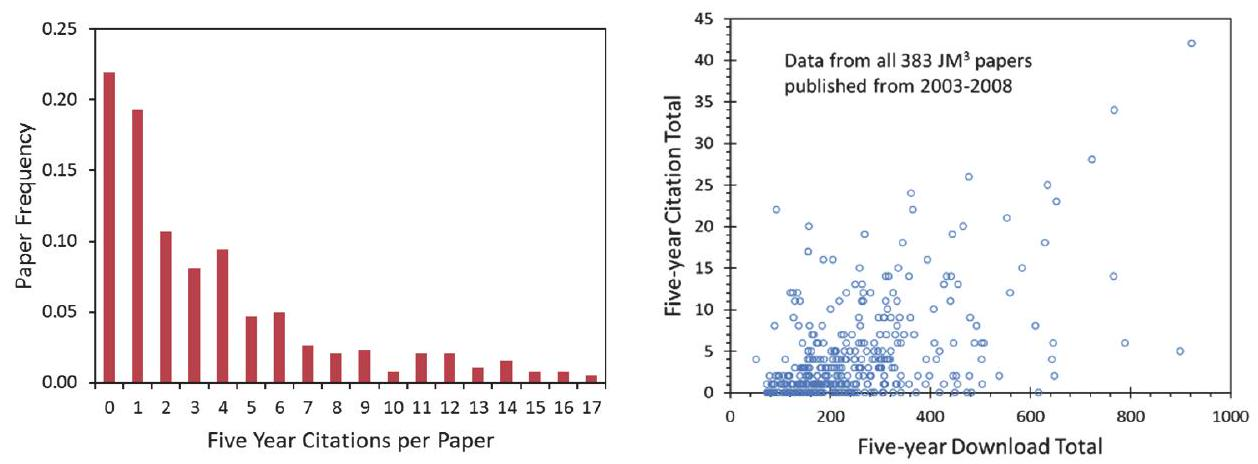
\includegraphics[max width=\textwidth, center]{2024_04_11_419211c3e451fc7cea07g-055}

Figure 7.1 Five-year citations and downloads for all $\mathrm{JM}^{3}$ papers published between 2003 and 2008.

\subsection*{7.4.2 In praise of the null result}
One unfortunate side effect of the search for significance is a bias against the null result. Almost all scientific studies look for effects: does input A affect output B?

The null result (also called the negative result) is simply a "no" in answer to that question. Theoretically, science should be neutral to the answer: no is just as good an answer as yes. But human nature does not usually work that way. In most cases, we study the effect of A on B because we want to see an effect. We want our new drug to have a positive impact on patient outcomes. We want our new process to result in better properties for the device being fabricated. There is almost always a preferred answer to the question "Does input A affect output B?"

In science, the only failed experiment is one that does not lead to a conclusion. Yet it is easy to think that an undesired conclusion is also a failure. One consequence of this very human tendency is a publication bias against the null result: journals are much more likely to publish papers that provide a positive result than ones that present a null or negative result.

The existence of a publication bias against null or negative results was first described in $1959,{ }^{4}$ and this bias has stayed the same ${ }^{5}$ or gotten worse since then. ${ }^{6}$ Many studies have shown that the vast majority of published scientific papers show positive results, that input $A$ does in fact affect output $B$ in the desired way. Negative results suffer from the "file-drawer" effect: a study that finds no impact or an undesired impact of A on B will likely be filed away in the researcher's desk drawer rather than published in a peer-reviewed journal. ${ }^{7}$ This leads to an incorrect impression that such experiments have never been tried.

There are three potential reasons for the existence of such a publication bias: editorial policy, reviewer bias, and author-submission bias. Although there may be some journals that actively discourage the publication of negative results through their editorial policy, such journals are probably the exception, and certainly $\mathrm{JM}^{3}$ is not among them. Reviewer bias is probably more common because reviewers are tasked with evaluating the significance of a manuscript, and there is often an unstated assumption that positive results are more significant than negative results.

Still, I think submission bias accounts for a majority of the publication bias. Authors, either anticipating a reviewer bias or having a bias for positive results themselves, are much more likely to submit a manuscript that contains positive results than negative results. A journal cannot publish a paper that demonstrates a null result if that paper is never submitted. The reasons for these biases are probably rational: positive results generally attract more readers and citations. The undesirable consequences of a bias against the null result, however, can be significant.

There are two major consequences of the publication bias against the null result, both unpleasant in their own way. The first is wasted effort. As I mentioned, most researchers are looking for positive results: they are trying to reduce the leakage current of a CMOS transistor, increase the Q-factor of a MEMS device, or reduce the roughness of a lithographically patterned feature. They try many different approaches, testing the effectiveness of many different variables. Most of the approaches do not work, but a few yield positive results. If the publication bias is at work, only the positive results are published, and the fact that certain experiments led to null or negative results remains unmentioned.

If readers remain unaware of these negative results, they are more likely to repeat these experiments in their own efforts to find positive results. The consequence is unnecessary waste. A completely valid and potentially important scientific outcome, that input A does not impact output B, is not published and so does not join the collective knowledge of the community. And the search for positive outcomes proceeds more slowly as a result.

The second consequence of the publication bias against null results is more insidious: it increases the likelihood that published results are wrong. In some cases, entire fields of study (such as extra sensory perception, ESP) publish only spurious positive results ${ }^{8}$ (a negative result, showing no evidence for ESP, would be unlikely to be published). But leaving aside such extreme cases, there is evidence that the publication bias against the null result leads to the frequent publication of spurious positive results in most or all fields, as John Ioannidis has persuasively claimed in his provocatively titled essay "Why Most Published Research Findings Are False"."

Consider twenty researchers all independently trying to see if input A affects output B. If A really has no impact on B, then one out of the twenty researchers will likely produce a spurious positive result to a $5 \%$ significance level $(\alpha=0.05)$ by pure chance. This will not cause any problems if all twenty researchers publish their results. But if the nineteen null findings remain unpublished (the file-drawer effect) and the one spurious positive result is published, readers will very reasonably assume that the results in the one published paper are representative of all studies and are likely to be true. The publication bias against the null result naturally leads to a degradation of the overall quality of published research as a whole. $^{10}$

However, science is supposed to be self-correcting, imbued with a "trust, but verify" mentality. Replication of results by other researchers should identify these spurious positive findings, eventually leading to sound conclusions. But "eventually" can be a long time. Further, there is some evidence that most scientific studies are never replicated, so bad results can linger in the collective consciousness of the scientific community for a very long time. ${ }^{4}$ The "publish or perish" mentality in academia, coupled with a publication bias against the null result, means that the scientific community often rewards impact and quantity over reproducibility and quality. Few scientists seem willing to devote significant time and resources towards replication of others' results.

Here is my modest proposal to help mitigate the negative impacts of a publication bias against the null result: when you write a paper and emphasize the positive results that you think are most important, please do not forget the negative or null results that you found along the way. Include a few sentences about the variables you tried that did not produce the desired effect. Show a graph of the data that demonstrates no significant effect, if for nothing else than to compare to the graph of data that does demonstrate the desired effect. Think about all the deadends and blind alleys that you went down in your search for a solution to your problem, then warn the rest of us about them. Consider the null result as a valid and important scientific discovery, and add it to your paper of positive results.

Reviewers and editors, do not recommend that null results be deleted from a paper just because they are null results. Although you may always consider the positive result to be more significant, do not automatically think that a null result is not important. Consider all of the wasted effort that can be avoided if just a few paragraphs of a paper are devoted to those null results that are almost always lurking around every scientific study.

\subsection*{7.5 Conclusions}
Journal editors are always looking for four things in every manuscript submitted to their journal: scope, quality, novelty, and significance. Before submitting your manuscript for publication, try evaluating it yourself using these four categories.

Because this book is about writing your paper, my advice here is to make it easy for a reader (and reviewer) to evaluate your work when reading your paper. Write so that it is clear what is the scope of your work, what is new and how it fits with prior published work, and why it is significant. And make the quality of your writing sufficiently high so that the reader can properly judge the quality of the science.

\section*{References}
\footnotetext{${ }^{1}$ M. Ware and M. Mabe, "The stm report", $3^{\text{rd }}$ ed., International Association of Scientific, Technical, and Medical Publishers, p. 5 (November 2012).

${ }^{2}$ D. J. de Solla Price, Little Science, Big Science, Columbia University Press, New York, pp. 8-19 (1963).

${ }^{3}$ P. O. Larsen and M. von Ins, "The rate of growth in scientific publication and the decline in coverage provided by Science Citation Index", Scientometrics 84(3), 575-603 (2010).

${ }^{4}$ T. D. Sterling, "Publication Decisions and the Possible Effects on Inferences Drawn from Tests of Significance - or Vice Versa”, J. Am. Statistical Assoc. 54(285), 30-34 (1959).

${ }^{5}$ T .D. Sterling, W. L. Rosenbaum, and J. J. Weinkam, "Publication decisions revisited: The effect of the outcome of statistical tests on the decision to publish and vice versa", The American Statistician 49(1), 108-112 (1995).

6 D. Fanelli, "Negative results are disappearing from most disciplines and countries", Scientometrics 90, 891-904 (2012).

7 R. Rosenthal, "The 'File Drawer Problem' and Tolerance for Null Results", Psychological Bulletin 86(3), 638-641 (1979).

8 D. J. Bem, "Feeling the future: experimental evidence for anomalous retroactive influences on cognition and affect", J. Personality Social Psychol. 100(3), 407-425 (2011).

9 J. P. A. Ioannidis, "Why Most Published Research Findings Are False", PLoS Med. 2(8), e124 (2005).

${ }^{10}$ J. P. A. Ioannidis, "Contradicted and Initially Stronger Effects in Highly Cited Clinical Research”, JAMA 294(2), 218-228 (July 13, 2005).
}
\section*{Chapter 8}
\section*{Picking the Right Journal}
A simmering question facing the scientist or engineer thinking about publishing a peer-reviewed paper is which journal to submit to. Hopefully, the question (and possibly its answer) is in the mind of the researcher from the beginning. Often, it is a last-minute choice after the paper is mostly or completely written. What factors should lead to a decision as to the most appropriate publication venue for your work? Historically, journal selection has involved relevance, acceptance rate, circulation, prestige, and publication time. ${ }^{1}$ But as more journals have moved online, and search engines have made finding and accessing articles much easier, some of these factors are less relevant today.

\subsection*{8.1 The Specialization Spectrum}
The first scientific journal was published over 350 years ago. ${ }^{2}$ The Philosophical Transactions of the Royal Society was a general journal of "natural philosophy" (as science was then called), and for over 100 years all regularly published journals were also similarly general. After all, there was no real specialization in science or scientists and so no need for specialized journals. The birth of chemistry as a modern scientific discipline changed that. Largely through the efforts of French scientist Antoine Lavoisier and colleagues, the "chemical revolution" of the late $18^{\text{th }}$ century helped make chemistry a quantitative science involving the combination of elements into molecules. In 1789, they started the first permanent specialty science journal, Annales de Chimie.

Since then, the growth of science has led inexorably to a growth in specialization, both in scientific disciplines and the journals that serve them. Today, there are about 30,000 peer-reviewed journals publishing more than 2 million articles a year. ${ }^{3}$ These journals run from the perfectly general to the highly specialized, but the vast majority of science journals today are specialized in narrow fields. The first decision facing prospective authors is where on the specialization spectrum they should try to publish.

Most science paper topics can fit well anywhere along a spectrum from the general to the specialized. To make this idea clear, I will fabricate a couple of example papers that could easily be published in the Journal of Micro/Nanolithography, MEMS, and MOEMS $\left(\mathrm{JM}^{3}\right)$. Suppose a paper was on th topic of measuring aberrations in an optical lithography tool. Such a paper would have a natural home in $\mathrm{JM}^{3}$, finding a large audience of lithographers interested in that topic. If, however, the measurement technique was applicable to lenses in general, not just lithographic lenses, the paper might be of interest to wider audience of optical scientists and engineers. Maybe a better home for such a paper would be a more general optics journal (SPIE's Optical Engineering comes to mind). But what if the measurement revealed a more subtle property of light with implications beyond lenses and aberrations? Could the paper be of interest to a more general audience of physicists? Or even to scientists in general?

The preceding questions address the specialization spectrum of science journals. As the following diagram illustrates for two example topics, almost any given subject can fit in many places along the specialization spectrum. At the top (most general) are the interdisciplinary science magazines, with famous journals like Science and Nature attempting to publish significant and timely research of wide interest. One step below are the general scientific disciplines such as physics, biology, chemistry, etc. They each have journals devoted broadly to those topics. The divisions to further subtopics can have multiple levels, depending on the size of the field. At the bottom are the most specialized fields, where further specialization is not practical due to the diminishing number of practitioners.

The key to deciding where to publish along the specialization spectrum is picking the target audience. Moving down the spectrum towards greater specialization will, in general, reduce the size of the overall audience but increase the interest match of the readers that remain. A large fraction of the readers of $\mathrm{JM}^{3}$ could be interested in a paper on photoresist dissolution, for example. What fraction of the readership of a polymer science journal would have a similar interest? Even more importantly, there may only be a very small overlap between the readership of the more- and less-specialized journals along the spectrum.
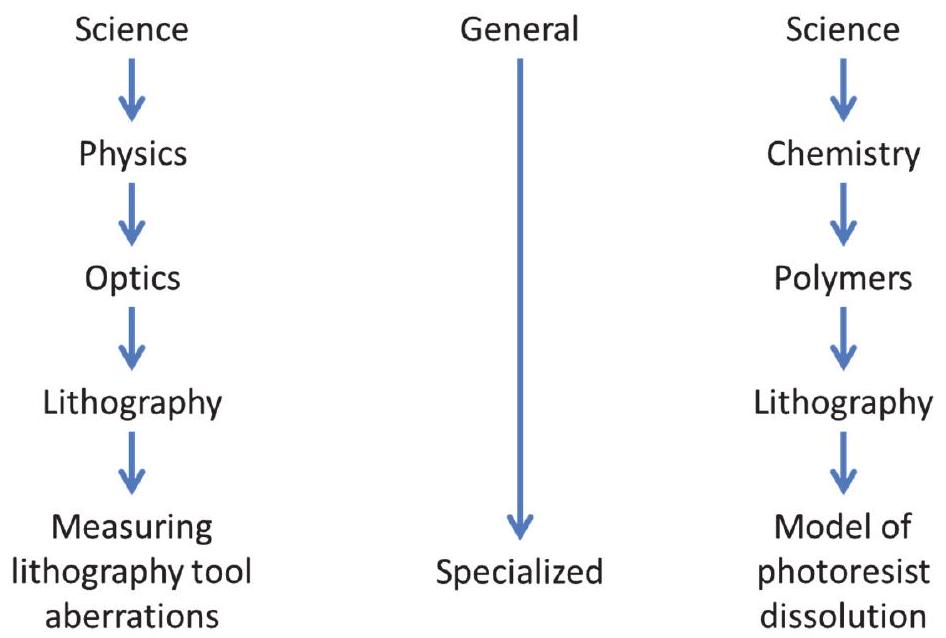
\includegraphics[max width=\textwidth, center]{2024_04_11_419211c3e451fc7cea07g-060}

Which readership would you rather reach: the photoresist users and chemists working in the field of lithography, or the more general polymer scientists working on a broader range of polymer topics?

There is no right answer to these questions because they depend specifically on the paper and the goals of the author. However, one thing is clear: moving up or down the specialization spectrum is not inherently better or worse. There is no doubt that the best general-science journals have higher levels of prestige, often associated with a higher journal impact factor. For many, prestige and peer recognition are prime motivations for publishing a paper. This thinking gives rise to what I consider to be a fallacious approach to picking a journal: send your manuscript to the one with the highest impact factor that you think may accept it. Often, this means moving as general in the specialization spectrum as your topic might allow.

The problem with this approach should be obvious: in the pursuit of a prestigious home for your paper, you may miss the audience you most want to reach. I think it is fair to say that there are many regular readers of a specialized journal who never pay attention to what is published in the more "prestigious" general-science journals. If reaching those specialized readers will cause your work to have greater impact on the community you hope to reach, then the specialized journal is probably the right place for your paper. Of course, the same can be said for any journal anywhere along the specialization spectrum. To achieve impact (rather than just impact factor), you must best match your ideal audience with a journal's actual audience.

\subsection*{8.2 Reading in the Age of Search Engines}
Critics of this audience-match approach to finding the best journal for a paper often point out that, in the age of Internet search engines, any reader can find any paper on any topic regardless of where it is published. And if this is true, why not use the somewhat vain criterion of prestige (and its proxy, impact factor) as the major factor for deciding where to publish?

Although there is some degree of truth in this position, I have a two-part response. First, search engines such as Google Scholar or DeepDyve, as powerful as they are, still tend to be blunt instruments when it comes to matching interested readers to the right papers. When a search provides me with a thousand hits in 0.13 seconds, I am often forced to manually filter results. And my first filter is, I think, quite common: Has the paper been published in a journal I recognize, one that I have already judged by reputation or past personal experience? With a few exceptions (famous journals like Nature or Physical Review), I know nothing about the impact factors of the journals I read. Instead, I know something about whether past pursuits of specific topics have profitably led me to those journals. For some topics, I may even go straight to the specialty journal I know first to do the search, knowing that my productive hit rate there is likely to be much higher than a general search.

Second, the match of journal scope to paper topic does more than make searches for papers more effective, it makes the publishing of those paper mor effective as well. After all, what makes peer review a value-added publishing process is the editorial peer review itself. Editors evaluate submissions, find reviewers, and then weigh reviews to both select papers for publication and improve those papers that are selected (see Chapter 10). The outcome of that process is a collection of published papers far improved from the collection that was originally submitted. But for this process to work as designed, the editors and reviewers must be properly matched to the topics of the submitted paper so that the label "peer" is in fact appropriate. And because editors and the reviewers they select are almost always found in the target audience for that journal, finding the best audience match for your manuscript will usually result in the best editorial process, the most appropriate reviews, and the most improvement in your paper.

\subsection*{8.3 Avoiding the Wrong Journal}
Unfortunately, the open-access movement in publishing (where authors pay for publication and readers can access the papers for free) has given rise to an ugly phenomenon: the predatory journal. These are sham scientific journals that pretend to be serving the needs of the scientific community but in fact are only about making money. Despite a legitimate-looking website and a reasonable-sounding name, these journals are not the real thing. They are rarely, if ever, read, will accept any paper submitted after a phony peer review, and then take the authors' money to put their paper up on a website. To publish a paper in a predatory journal is worse than a waste of money, it is a blot on the author's career and a detriment to science.

To avoid predatory journals, here is a list of questions to ask before submitting an article to a journal that you are not familiar with (adapted from the \href{http://thinkchecksubmit.org}{thinkchecksubmit.org} website):

\begin{itemize}
  \item Do you or your colleagues know the journal?
  \item Have you read any articles in the journal before?
  \item Is it easy to discover the latest papers in the journal?
  \item Can you easily identify and contact the publisher?
  \item Is the publisher name clearly displayed on the journal website?
  \item Can you contact the publisher by telephone, email, and post?
  \item Is the journal clear about the type of peer review it uses?
  \item Are articles indexed in services that you use?
  \item Is it clear what fees will be charged?
  \item Does the journal site explain what these fees are for and when they will be charged?
  \item Do you recognize the editorial board?
  \item Have you heard of the editorial board members?
  \item Do the editorial board members mention the journal on their own websites? (Sometimes people are listed as editorial board members without their permission.)
  \item Is the publisher a member of a recognized industry initiative?
  \item Do they belong to the Committee on Publication Ethics (COPE)?
  \item If the journal is open access, is it listed in the Directory of Open Access Journals (DOAJ)?
  \item If the journal is open access, does the publisher belong to the Open Access Scholarly Publishers' Association (OASPA)?
  \item Is the journal hosted on one of INASP's Journals Online platforms (for journals published in Bangladesh, Nepal, Sri Lanka, Central America and Mongolia) or on African Journals Online (AJOL, for African journals)?
  \item Is the publisher a member of another trade association?
\end{itemize}

Be careful of the growing number of predatory journals and avoid adding to their plague on science.

\subsection*{8.4 Conclusions}
In summary, picking a journal to submit a manuscript for publication is a very important decision, one that deserves careful consideration. The best decision process involves two steps:

\begin{itemize}
  \item What is the ideal audience for your paper?
  \item Which journal has a readership that is best matched to this ideal audience?
\end{itemize}

Following this process almost always provides an additional benefit: the resulting journal editors are usually the best ones to evaluate and help improve your work.

As always, I advocate a reader-centered process of writing and publishing papers. If you keep the readers in mind as your first priority, picking the right journal for publication becomes a fairly straightforward task. Because a readercentered process of writing leads to a paper written for the needs of the audience, it is important to have a target journal in mind at the start of the writing process rather than delaying such a decision until the paper is nearly finished.

Alas, many authors approach writing and publishing from an almost opposite perspective: how to best serve the needs of the author. The result is often an emphasis on quantity rather than quality, and getting the work into the hands of people most likely to reference the work rather than use the work. There should be (and often is) a great deal of overlap between what is best for the reader and what is best for the author. But finding an "and" solution (good for both author and reader) sometimes requires more effort than finding an "or" solution (good for either author or reader). The effort is worth it.

Finally, time to publication will always be an additional factor when publishing cutting-edge research. $\mathrm{JM}^{3}$, like most journals, continues to mak progress in this area, with a median time from submission to first decision of 5 weeks and a median time from final decision to publication of about 3 weeks. If your work requires timely publication, try to find these numbers for the journal you are considering.

\section*{References}
${ }^{1}$ A. C. Weller, Editorial Peer Review: Its Strengths and Weaknesses, ASIS\&T, Medford, New Jersey, p. 130 (2001).

2 C. A. Mack, "Editorial: 350 Years of Scientific Journals", J. Micro/Nanolith. MEMS MOEMS 14(1), 010101 (2015).

${ }^{3}$ M. Ware and M. Mabe, "The stm report", $3^{\text{rd }}$ ed., International Association of Scientific, Technical and Medical Publishers, p. 5 (November 2012).

\section*{Chapter 9}
\section*{Cover Letter}
Whenever a manuscript is submitted to the Journal of Micro/Nanolithography, MEMS, and MOEMS $\left(\mathrm{JM}^{3}\right)$, the manuscript first goes to me, the Editor-in-Chief. And the first thing I do is read the cover letter that accompanies the manuscript. Thus, the cover letter creates the first impression that I have of the manuscript. Is this important? Of course I think it is, but let me explain why the author(s) should think it is important as well.

\subsection*{9.1 The Purpose of the Cover Letter}
When I look at a submission, my first decision is whether I think it would be productive for the manuscript to go through the peer-review process or if it should be declined without review. The cover letter gives me the information I need to make this first important assessment (or at least it should). If I believe the manuscript merits review by $\mathrm{JM}^{3}$, my next choice is which senior editor to send it to, based on a match of editor expertise to paper topic. The senior editor will then repeat my exercise, deciding whether to decline without review or, if not, which associate editor to assign it to. Finally, the associate editor will again read the cover letter and could again decide to decline without review. If the associate editor believes the material merits review, he or she must find the right reviewers for the manuscript. Each editor might look at the full manuscript and may even read it fully and carefully. But it is the cover letter that is the first and most important indicator that each editor looks at when making these decisions.

Why might a manuscript be declined without review? There are three basic reasons. First, the paper may not fit within the scope of our journal. I have declined perfectly good manuscripts because they would be better served by being published in a different journal (if possible, I try to recommend a more appropriate journal and encourage the authors to try there). Another reason to decline without review would be if the manuscript's English is poor. I have great respect for anyone who writes a paper in a language that is not their first, native language - this is something I am totally incapable of doing. But if reviewers have too much difficulty understanding the meaning of the sentences, they will not be able to adequately review the technical merits of the work. I would not waste the precious time of our volunteer reviewers unless I believe that the content of the manuscrip is clear enough to be understood. If I decline for this reason, I encourage the authors to have the manuscript edited by a native English speaker (or, optionally, by a commercial editing service) and then resubmit. Finally, an editor may decline a paper without review if it is clear that the paper is either not novel or not significant.

Thus, the author's goal in writing the cover letter should be obvious: provide enough information to ensure that the manuscript is not inappropriately declined without review. With this in mind, here are my recommendations on how to write a good cover letter.

\subsection*{9.2 A Structured Cover Letter}
A cover letter is formatted like a standard business letter and addressed to the Editor-in-Chief. It should be succinct and focused-not longer than one page, containing everything needed for the editors to make the "decline/send out for peer review" decision.

I am a big fan of structured abstracts (see Chapter 6), where the important topical areas needed in the abstract are formalized by adding subheadings and subsections (the "structure"). Borrowing from that idea, a predefined structure can make the cover letter more effective. Start with a standard business letter opening/greeting. Then, in the body, supply the following structure, with one or at most two sentences for each topic:

Manuscript information: Title of the submitted manuscript and type of article (letter, regular paper, special section paper, review, tutorial, communication, etc.). If submitting to a special section, mention the special section name.

Problem being addressed: What issues led to this work? What gap is being filled? What is the broader context for this work?

Novelty of the work: What is new here, not previously published? "To our knowledge, this is the first report showing...."

Significance of the work: Why is the novel content mentioned above important? What is the potential impact to the field?

Fit to this journal: Why does this work belong in and appeal to the readership of this journal? How will publication of this manuscript benefit the journal? (Be familiar with the journal scope.) Mention if this paper builds on a previous paper published in this journal or is otherwise directly linked to a paper published in this journal.

Double publication: "This manuscript has not been previously published and is not currently in press, under review, or being considered for publication by another journal."

Author approval: "All authors have read and approved the manuscript being submitted, and agree to its submittal to this journal."

Finally, end with a standard letter ending, including the name and contact information for the corresponding author.

Things to avoid in a cover letter include statements that exaggerate or overstate results, conclusions that are not supported by the data reported in the manuscript, sentences repeated word-for-word from the manuscript text (please do not copy and paste the abstract!), and too many technical details. Remember that the cover letter should be brief-say only what is most important.

While I like the format of a structured cover letter, authors are free to use a more conventional prose approach. Be sure to include all of the information outlined previously. Some journals also request that recommendations for reviewers for the manuscript also be included in the cover letter. For other journals, those recommendations can be made during the online submission process, and so their inclusion in the cover letter is not needed.

\subsection*{9.3 Conclusions}
The requirement of providing a cover letter is not arbitrary-it is an important part of the manuscript submittal and review process. A well-crafted cover letter will smooth the review process by making sure that an inappropriate "decline without review" decision is not made, and help to find the best editors and reviewers for the manuscript, thus speeding it through the process and producing the most desirable outcome. Considering all of the effort that goes into preparing a manuscript for publication, it would be a shame for that manuscript to receive less than a fair shake simply because of a poorly crafted cover letter.

\section*{Chapter 10}
\section*{The Editorial Review Process}
Peer review is a critical part of the publishing process at most science journals. Yet for many authors, the editorial review process might seem intimidating, maybe even a bit mysterious. Because there are many variations on the basic peer-review paradigm, in this chapter I will explain in some detail how the process works at the Journal of Micro/Nanolithography, MEMS, and MOEMS ( $\left.\mathrm{JM}^{3}\right)$. It is typical of other peer-review processes as well.

Peer review is defined as "the critical assessment of manuscripts submitted to journals by experts who are usually not part of the editorial staff." It supports the scientific process by providing authors with constructive criticism of their work and by filtering out less valuable work, thus providing a "stamp of approval" from editors and peers for published scientific work. The mere prospect of peer review prompts authors to improve both the science and its presentation in a submitted manuscript.

\subsection*{10.1 The Goals of Peer Review}
The peer-review process serves two immediate goals: to help editors decide which manuscripts to publish and which to reject (filtering), and to give authors advice on how to improve their papers (criticism). Additionally, the "stamp of approval" of being published in a peer-reviewed journal can aid authors in their careers, as well as having many other benefits. But it is my philosophy that everything about the science publishing enterprise should be focused on the reader, and so it is with the peer-review process. The filtering and criticism that accompanies an editorial peer-review process helps to get the best papers into the hands of the most interested readers efficiently.

But for the peer-review process to fulfill its goals, the reviews must be of good quality. What constitutes a quality review? Alas, almost none of us have ever been trained in proper paper reviewing - we generally figure it out through experience. Anyone who has published a fair number of papers knows that some reviews are of much higher quality than others (independent of the ultimate fate of any given manuscript). A good review teaches the author about writing and about science, resulting not only in one better paper but in making every subsequent paper th author writes better. It also makes the job of the editor significantly easier. A poorquality review does none of this.

\subsection*{10.2 Characteristics of a Well-Done Review}
The topics of this book constitute a reasonable list of things a reviewer should be looking for in any paper that might hope to be published. The appendix is a summary of the advice from this book, organized in the form of a checklist.

To be clear, neither editors nor reviewers need to use a formal checklist when writing a review. The appendix is a guideline to help both editors and reviewers make sure that the most important aspects of a scientific paper are considered. As one might expect, the checklist also happens to be great list of things an author should consider before submitting a manuscript. It is always good advice for an author to think like a reader, and the first readers will be the editors and reviewers.

After reading and critically evaluating a manuscript, the reviewer must now convey that evaluation to the journal editors. In all cases, a respectful and constructive tone should be used. The format of the review is not important, but each review should contain certain vital information. The first paragraph should contain these three key points:

\begin{itemize}
  \item Provide a brief (1-2 sentence) synopsis of the paper;
  \item Explain what is novel in this paper (1-2 sentences), both what the authors claim and your assessment; and
  \item Explain why the work is significant or not (1-2 sentences).
\end{itemize}

If the reviewer finds it difficult to put any or all of these points into one or two sentences, chances are the manuscript has not done a good job conveying its key messages - a potential red flag.

The second paragraph should give an overview of the quality of the research being reported. If there are any significant flaws in the logical progression from method to data to analysis to conclusions, bring them up here and what could be done to fix the flaws. In this paragraph, focus on the big issues (if there are any). If all is good, say so.

The third and final section of the review should be a list of specific points that the author should address. These points can be small or large, from graphics formatting to paper organization. Remember, though, that copyediting will be done by the journal staff after acceptance, so do not worry about language or format issues unless they interfere with your ability to properly understand and review the manuscript, or if improper language causes what is said to deviate from what is meant.

What does a poor-quality review look like? A list of generic complaints or conclusions without specific references to the details of the manuscript is not very helpful (for example, saying that the work is not novel without providing any example prior publications that cover the same topic). The worst kind of review is one that simply states the reviewer's accept/reject opinion. This is essentially of no value to an editor.

Reviewers are absolutely essential to the success of a peer-reviewed scientific journal. Reviewers volunteer their valuable time (typically 3-8 hours per manuscript) for no obvious benefit other than the altruistic goal of giving back to their community.

\subsection*{10.3 The Peer-Review Process at $\mathrm{JM}^{3}$}
$\mathrm{JM}^{3}$ practices an editor-driven external peer review of author-submitted manuscripts. Reviewers (also called referees or assessors) are anonymous, meaning that authors never know the identity of the reviewers. This single-blind approach is not the only style in use at scientific journals. Some journals practice double-blind reviewing, where the reviewers are not told the names or institutions of the authors (in an attempt to avoid bias). Other journals practice open review, where the names of the reviewers are published along with their reviews when the paper is published. Other journals take a middle road, where reviewers are given the option of signing their reviews before they are sent to the authors. The singleblind process used by $\mathrm{JM}^{3}$ (and described in some detail in this section) is by far the most common style of peer review in scientific publishing. ${ }^{2}$

Journals should have a well-documented process for peer review. Here is a step-by-step description of the manuscript review process used by $\mathrm{JM}^{3}$ :

\begin{enumerate}
  \item Authors submit their manuscript online, along with a cover letter and various other information. During this step, the author selects either a currently open special section or a regular paper or letter category for their manuscript.

  \item The manuscript goes through a quality-control check by journal staff. If there were problems with the submission, then the journal staff works with the corresponding author to address them.

  \item The manuscript is processed through the Similarity Check plagiarism screening service (based on software from iThenticate), comparing the submission to a large database of previously published papers. If there is sufficient content in the submission that is identical to that found in a previously published paper, the authors will be contacted for an explanation, and the manuscript may be rejected and sanctions imposed if egregious problems are confirmed.

  \item Based on the category selection made during submission, the manuscript goes to either the special-section Guest Editors or the Senior Editor (SE) associated with the regular paper category. The editor performs a first editorial review by reading the cover letter, title, and abstract, and skimming through the paper. This editor checks to see if the scope of the paper properly matches the scope of the journal and if the writing i sufficiently good to allow for an effective review. If not, the editor may decide to decline the manuscript without review.

  \item For a regular submission, the SE decides on an Associate Editor (AE) with suitable expertise to handle the submission. The $\mathrm{AE}$ is not necessarily an expert on the topic but will have enough familiarity to be able to find reviewers and interpret their reviews. For a special section submission, the Guest Editors will decide which Guest Editor will serve the role of the AE for this submission.

  \item The $\mathrm{AE}$ does the bulk of the editorial work for $\mathrm{JM}^{3}$. They begin by performing a second editorial review of the paper, checking for scope, novelty, significance, and quality. They may skim the paper quickly or read it in great detail. The AE must decide if the paper has a chance of being accepted for publication and thus is worth sending out for review.

  \item If the $\mathrm{AE}$ does not decide to decline the manuscript without review, they will search for and assign qualified reviewers. At least two reviews are required to accept a manuscript for publication, but some AEs may choose to seek three reviews. Often, the reviewers are chosen to have complementary skills (experimental, theoretical, mathematical, etc.) so that the full range of topics in the manuscript can have expert analysis. Authors have the opportunity to supply a list of suggested reviewers at the time of submission, but it is the AE's decision whether to use anyone from that list. Finding qualified reviewers is the often most difficult and problematic step in the process, and sometimes 10-20 candidates must be asked before two reviewers accept the task.

  \item When the reviews have been returned, the $\mathrm{AE}$ evaluates the reviews and makes a decision (usually to request author revisions or reject). Although the reviewers may provide accept/reject advice, the AE makes the final decision based on their reading of the manuscript and the substance of the reviews.

  \item If the author revises the manuscript, it is sent back to the same AE. The AE looks over the revised manuscript and the author's point-by-point response to the reviewers' comments, and either decides to send the manuscript out for re-review or makes an accept/reject decision at this point. Multiple rounds of re-review are possible, depending on the extent of the revisions. Generally, the manuscript would be sent back to the same reviewers, but it is possible that new reviewers would be chosen if an original reviewer was unavailable or if significant added material required a reviewer with an additional area of expertise.

  \item Finally, after a manuscript decision has been made, the proposed decision is sent to the Editor-in-Chief for approval. The Editor-in-Chief performs a final quality check on the overall editorial process, possibly making suggestions for changes or improvement. At $\mathrm{JM}^{3}$, it is rare that I change in any way the decision made by the $\mathrm{AE}$.

  \item If the manuscript is accepted, the authors receive instructions about how to make a final submittal of the manuscript and its figures. No changes to the manuscript content should be made following acceptance.

  \item The final submitted manuscript goes through copyediting and professional composition steps. These important and often unheralded steps can have a major impact on the level of professionalism of the paper, fixing typos and grammatical errors, improving the exposition and presentation of the paper, and ensuring that the graphics are of sufficient quality.

  \item Page proofs are sent to the corresponding author for approval, and possibly to supply missing information. Authors should return these proofs promptly.

  \item The finalized paper is published online immediately and in the print version of the journal at the end of the quarter.

\end{enumerate}

$\mathrm{JM}^{3}$ has a specific process for handling submissions by members of the editorial board (myself included) to ensure an impartial review, treating the editorial board member as any other author, with no access to the internal editorial process for that submission. Additionally, $\mathrm{JM}^{3}$ accepts appeals from authors who disagree with an editorial decision. The Editor-in-Chief is available to hear from authors or reviewers who wish to lodge complaints or make suggestions for improving the publication process.

Here are some of the major statistics for $\mathrm{JM}^{3}$ in 2016:

\begin{itemize}
  \item 134 manuscripts were received (114 regular papers, 13 special section papers, and 7 letters)
  \item For regular submissions (papers and letters),
  \item $18 \%$ were declined without review.
  \item $21 \%$ of manuscripts were rejected after being reviewed.
  \item The overall acceptance rate was $61 \%$.
\end{itemize}

○ The average time to first decision was 5.5 weeks (median time was 5.1 weeks).

\begin{itemize}
  \item No papers were accepted without revision, $65 \%$ of accepted papers were revised by the authors once, $30 \%$ were revised twice, and $5 \%$ were revised three times.
\end{itemize}

For papers that were accepted, the average time to acceptance was 15.6 weeks, and the median was 13.6 weeks (which includes the time for author revisions). Each additional revision cycle added about 2 weeks on average to the final acceptance time. The average (median) time from acceptance to publication was 3.6 (3.4) weeks.

\subsection*{10.4 Responsibilities}
All parties in the peer-review process (authors, editors, and reviewers) must work in an environment of mutual trust and cooperation. Honesty and integrity are of course required in all aspects of the process. Additionally, each participant in the peer-review process has specific responsibilities that must be fulfilled.

\section*{Authors}
\begin{itemize}
  \item Ensure that the work is original and has not been previously published or submitted for publication elsewhere (see Chapter 15). Cite your own prior and overlapping work properly (see Chapter 5).
  \item Select the list of authors appropriately (see Chapter 13), with full approval of the submission by all authors.
  \item Choose the most appropriate journal (see Chapter 8) and submit the best manuscript possible. Never knowingly submit a poor manuscript hoping that the editors and reviewers will help you fix it.
  \item Spend the time to understand the submission requirements of the chosen journal and comply with those requirements.
  \item Identify all funding sources and make the editors aware of any potential conflicts of interest.
\end{itemize}

\section*{Editors}
\begin{itemize}
  \item Provide a transparent process for editorial review, and deviate from that process only under exceptional circumstances.
  \item Deal fairly and respectfully with all parties in the publishing process.
  \item Recuse yourself when dealing with a manuscript for which you have a conflict of interest-let a non-conflicted editor handle the submission and make the decisions.
  \item Ensure that all details of a submission are kept confidential.
  \item Work assiduously for timely decisions.
  \item Choose reviewers who are likely to provide fair, unbiased, high-quality, and timely reviews.
  \item Hold all parties in the publishing process to the highest ethical standards. ${ }^{1,3}$
\end{itemize}

\section*{Peer Reviewers}
\begin{itemize}
  \item Disclose any conflicts of interest (arising from competitive, collaborative, financial, or other relationships) that might bias your opinions of the manuscript. If you are chosen to review despite a conflict of interest, do your best to provide an unbiased review.
  \item Return the review quickly. If you are unable to return a quality review in a timely manner for any reason, let the editors know as soon as possible.
  \item Provide a constructive, professional review-it should never get personal.
  \item Provide a detailed review, supporting all opinions with evidence; your goal should be to help the authors improve their paper even if you recommend rejection.
  \item Hold information gained from your review confidential. Never disclose or use knowledge gained from reviewing a manuscript until that manuscript has been published.
\end{itemize}

\subsection*{10.5 Criticisms of the Peer-Review Process}
The peer-review process has its critics, some of them quite vocal. Here are some of the major criticisms often leveled against the peer-review process: ${ }^{4,5}$

\begin{itemize}
  \item It stifles innovation by rejecting non-conforming or controversial views, ${ }^{6,7}$ and distorts the record by rejecting null results (see Chapter 7).
  \item It is unreliable, frequently failing to find major flaws in the work, including fraud and plagiarism.
  \item It is neither consistent nor objective, and it is often biased in several ways. ${ }^{8}$
  \item It is expensive and delays publication.
  \item There is little evidence that it is effective, let alone the best method available.
  \item Most rejected articles are eventually published in another peer-reviewed journal.
\end{itemize}

I have to admit that each one of these points has some validity. The peer-review process is not, and never will be, perfect. However, there is a growing body of evidence that peer review works in its intended goals of filtering and improving papers. ${ }^{9-11}$ A recent survey found that $91 \%$ of authors thought the peer-review process had improved their last published paper. ${ }^{12}$ There are many flaws in the process, but as former $B M J$ editor Stephen Lock wrote, "we have no better way of distinguishing between the promising and the meretricious or for improving the scientific and linguistic qualities of an article." 5

\subsection*{10.6 Conclusions}
Peer review has evolved significantly since it was first introduced in the mideighteenth century, ${ }^{13,14}$ and it continues to evolve today. Technology has drastically sped the process, with email, web-based submissions, and online publishing. Search-engine-style document comparisons do a reasonable job of detecting plagiarism. But in the end, it is the careful reading of a manuscript by editors and expert reviewers that makes the whole process work. Science is a human endeavor, with the scientific quality dependent on the attitude, training, and work ethic of the scientists involved. Likewise, scientific journal publishing depends on the efforts of well-trained and hardworking scientists and engineers who choose to give back to their scientific community by volunteering for their journal.

\section*{References}
\footnotetext{${ }^{1}$ International Committee of Medical Journal Editors, "Recommendations for the Conduct, Reporting, Editing, and Publication of Scholarly Work in Medical Journals” (2014).

2 I. Hames, Peer Review and Manuscript Management in Scientific Journals, ALPSP/Blackwell Publishing, Malden, MA (2007).

${ }^{3}$ Committee on Publication Ethics, "Code of Conduct and Best Practice Guidelines for Journal Editors”, version 4 (2011).

${ }^{4}$ D. Rennie, "Editorial Peer Review: Its Development and Rationale," Chapter 1 in Peer Review in Health Sciences, F. Goodlee and T. Jefferson, Eds., BMJ Books, London, 3-13 (1999).

${ }^{5}$ S. Lock, A Difficult Balance: Editorial Peer Review in Medicine, BMJ, London (1985).

6 J. M. Campanario, "Have Referees Rejected Some of the Most-Cited Articles of All Times?”, J. Am. Soc. Inform. Sci. 47(4), 302-310 (1996).

${ }^{7}$ J. M. Campanario and E. Acedo, "Rejecting Highly Cited Papers: The Views of Scientists Who Encounter Resistance to Their Discoveries From Other Scientists”, J. Am. Soc. Inform. Sci. Tech. 58(5), 734-743 (2007).

${ }^{8}$ C. J. Lee, C. R. Sugimoto, G. Zhang, and B. Cronon, "Bias in Peer Review", J. Am. Soc. Inform. Sci. 64(1), 2-17 (2013).

${ }^{9}$ T. Jefferson, M. Rudin, S. B. Folse, and F. Davidoff, "Editorial peer review for improving the quality of reports of biomedical studies", Cochrane Database of Systematic Reviews, Issue 2, 1-39 (2007).

${ }^{10}$ R. H. Fletcher and S. W. Fletcher, "The Effectiveness of Journal Peer Review", Chapter 4 in Peer Review in Health Sciences, F. Goodlee and T. Jefferson, Eds., BMJ Books, London, 62-75 (1999).

${ }^{11}$ A. C. Weller, Editorial Peer Review: Its Strengths and Weaknesses, ASIS\&T, Medford, NJ (2001).

12 A. Mulligan, L. Hall, and E. Raphael, "Peer Review in a Changing World: An International Study Measuring the Attitudes of Researchers", J. Am. Soc. Information Sci. Technol. 64(1), 132-161 (2013).

${ }^{13}$ H. Zuckerman and R. K. Merton, "Patterns of Evaluation in Science: Institutionalisation, Structure and Functions of the Referee System”, Minerva 9(1), 66-100, (1971).

${ }^{14}$ C. A. Mack, "Editorial: 350 Years of Scientific Journals", J. Micro/Nanolith. MEMS MOEMS 14(1), 010101 (2015).
}
\section*{Chapter 11}
\section*{Review Articles}
For a regular contribution to a peer-reviewed scientific journal, a paper must meet four criteria before it is publishable:

\begin{itemize}
  \item The content of the paper must match the scope of the journal,
  \item The quality of the paper (method and execution of the research, as well as the writing) must be sufficiently high,
  \item It must present novel results (with the exception of review papers and the like), and
  \item The results must be significant enough to be worth reading about (and thus worth publishing).
\end{itemize}

An exception is made for the third requirement, novelty, for an important category of papers: the review article. Review articles, as the name implies, provide a critical evaluation of previously published work on a specific topic. Reviews tend to be quite popular with readers because they pack a lot of information in a small space, giving readers a great return on their invested time. They are a gift. Most readers do not have the time or inclination to thoroughly research the full literature on a specific topic and so greatly appreciate it when an author reports on the results of their thorough review of the topic. "Mini-reviews" are becoming increasingly popular as well (more on that in Section 11.3).

\subsection*{11.1 What is a Review Article?}
A review paper provides an organization and synthesis of past work on a topic around a specific theme. What a review paper is not is a list of papers on a specific topic with a short summary of the important ones. Every review paper should have a story to tell, a theme, and a point of view. It should be idea-driven, not literaturedriven or author-centric. Here are some of the most common themes found in the best review papers:

\begin{itemize}
  \item A controversy: two or more camps with competing theories or explanations of a phenomenon, with evidence for each.
  \item Progress towards the development of a major new tool, process, method, or theory.
  \item Historical development leading to a major discovery or concept, and its implications for today and the future.
  \item Comparison of different approaches toward the measurement/design/ fabrication/modeling of a specific thing of importance, and their advantages and disadvantages.
  \item The use of a specific tool/process/method across disciplines or for different applications.
  \item A novel insight gained from a wider view of recent progress on a topic, or the recognition of a critical new problem or issue previously unnoticed.
  \item A call to action: why the community should devote considerable resources to a certain topic.
\end{itemize}

The major goal of every review should be to achieve an organization and synthesis of past work around the chosen theme in order to accelerate the accumulation and assimilation of recent knowledge into the existing body of knowledge. A review provides order to what otherwise might appear to be a chaotic blast of recent research results. Thus, while a review paper may not present novel results, it almost always presents a novel meta-analysis of results leading to a novel organization and synthesis.

\subsection*{11.2 The Structure of a Review Article}
Once a theme is chosen, the real work of a writing a review paper begins with a comprehensive literature review. In some sense, the citations found in the review are the point of the article because they tell the reader what work is being synthesized. One can only organize and synthesize the work one is aware of, and nothing exposes the flaws of a review like missing references. Keep in mind that a review topic that is too broad is often less valuable than a review topic that is too narrow. ${ }^{1}$ Focus is essential to success in a review article.

The introduction of a review article is similar to the introduction to a research article (see Chapter 2). It begins with a description of the background topic and why that topic is significant. It states the gap in the knowledge of that topic that has recently been filled with the work that is about to be reviewed. It then outlines the theme of the current review (the controversy, progress, historical development, etc.) and how it fits into that topic and its knowledge gap. It is important that the introduction clearly defines the scope of the review so that the reader knows what is included and what is excluded from consideration.

The structure of the middle sections of a review paper is designed for the story being told and thus depends greatly on the theme chosen for the review. A good writer will let the story guide the flow of the review, always keeping in mind th goals of organization and synthesis. Presenting results in chronological sequence is only appropriate if the theme of the review is one of historical development.

Like the introduction, the concluding section of a review paper is similar to that of a research paper. Conclusions generalize, looking for the bigger lessons that can be taught. After a very brief summary of the review and its primary message, one should highlight the implications of the reviewed work and point out the gaps still found in our current knowledge. Generally, the reader then expects a description of future work needed and future questions to be answered. It is good to end with some speculation, so long as it is labeled as such.

\subsection*{11.3 What Makes a Review Article "Good"?}
Like a research article, the goal of the review article is to teach: "Good writing is good teaching." ${ }^{.2}$ Good scientific writing always strives for accuracy and clarity, and that is certainly true for review articles as well. Remember that the audience for a review article is wider than the audience for any of the articles that you cite in your review. Thus, try to make sense of the literature that you cite to this wider audience.

Reviews should be critical but even-handed, and not just accepting of all previously published conclusions. But do not get personal: when criticizing, always criticize the work, not the authors. And remember that science progresses slowly and unevenly, in fits and starts. Be sympathetic to the many wrong turns that litter the final path to understanding. ${ }^{3}$

Generally, the author(s) will include their own work as a part of the review. After all, the authors are generally experts in the field being reviewed because they have contributed to that field. To mitigate this perceived conflict of interest, a difficult and careful balance must be achieved when fitting the author's own work into the overall literature of the field. An objective analysis of one's own work is very hard to pull off, so admitting as much is a good first step.

Writing a review article tends to be a lot of work. They are typically twice as long as most regular journal articles, with hundreds of references. Many experienced authors have one or more review papers hidden away within them, but there is often too little time to get them out. This is where the mini-review comes in. Mini-reviews tend to focus on a recent "hot topic" that has only a limited amount of accumulated literature. They tend to be about half the length and number of citations as full reviews due to their narrower scope. Still, they can be very valuable to readers if they accomplish the twin goals of organization and synthesis.

\subsection*{11.4 Conclusions}
If you want to write a review paper, the first step is to decide on the theme (story) of the paper. This helps to define the scope of the review, which then drives the literature search that must begin any such effort. The unique (even novel) contribution that the author of a review paper can make is the organization and synthesis of the knowledge found in the literature. Thus, deciding upon this organization and executing on the synthesis of the past work is where the author truly add value with their review. The authors of a good review paper deserve huge thanks from the many readers who benefit from their efforts - we need more of such efforts.

\section*{References}
${ }^{1}$ M. Pautasso, "Ten Simple Rules for Writing a Literature Review”, PLoS Comput Biol. 9(7), E1003149 (2013).

${ }^{2}$ D. J. Bem, "Writing a Review Article for Psychological Bulletin", Psychological Bulletin 118(2), 172-177. (1995).

${ }^{3}$ J. Webster and R. T. Watson, "Analyzing the Past to Prepare for the Future: Writing a Literature Review," MIS Quarterly 26(2), xiii (2002).

\section*{Chapter 12}
\section*{The Ethics of Scientific Publication}
As mentioned many times throughout this book, the main ethos of paper writing in science is to make the paper reader-centric, not author-centric. But readers can be thought of as a proxy for science as a whole, so that making a paper readercentric is equivalent to putting the advancement of science first. The goal is to advance science by writing a paper that adds novel scientific content to the existing communal collection of scientific knowledge. Almost all of the advice found in this book supports that goal.

There can be other goals in science writing, self-interested goals that benefit the author (see Chapter 1). There is nothing fundamentally wrong with selfinterest, unless these additional goals come in conflict with the main goal of scientific advancement. Unfortunately, they sometimes do. As a result, it is wise for authors to always keep their ethical responsibilities in mind throughput the process of researching, writing, and publishing. If the advancement of science always remains as each author's primary goal, conflicts will usually work themselves out.

\subsection*{12.1 The Primary Ethic of Scientific Publication}
For a result to be scientific, and contribute to the body of scientific knowledge, it must be described sufficiently so that the paper's conclusions can be validated by others. I call this the primary ethic of scientific publication. It requires openness, honesty, and integrity on the part of the authors, all traits that most scientists readily exhibit. When followed, this ethic allows new scientific knowledge to add to existing knowledge and for science to advance.

When commercial or competitive interests intrude, there may be pressure on authors not to provide sufficient detail in a paper. Companies may want to keep certain ideas trade secrets. Authors may want to keep flaws hidden, to increase the chance of publication and to maximize claims of significance. Authors may also want to keep certain techniques to themselves in order to keep ahead of rival research groups in generating new results. Secrets may be desirable, or even necessary, but they are not a part of science.

Put simply, if other interests require that details necessary to validating a paper's conclusions cannot be disclosed, then that paper should not be published in a peer-reviewed journal. Authors who want to keep necessary details hidden should not submit such work for publication.

\subsection*{12.2 Author Responsibilities before Publication}
Before submitting a manuscript to a peer-reviewed journal for publication, here are the major responsibilities of the authors:

\begin{itemize}
  \item Carry out the research leading to publication in an ethical manner. ${ }^{1}$
  \item Write your paper with openness and honesty, keeping the primary ethic of scientific publication in mind.
  \item Cite as you write to avoid plagiarism through sloppy citation practice (see Chapter 14).
  \item Ensure that the work is original and has not been previously published or submitted for publication elsewhere (see Chapter 15). Cite your own prior and overlapping work properly (see Chapter 5).
  \item Select the list of authors appropriately (see Chapter 13), with full approval of the submission by all authors.
  \item Choose the most appropriate journal (see Chapter 8) and submit the best manuscript possible. Never knowingly submit a poor manuscript with the hope that the editors and reviewers will help you fix it.
  \item Spend the time to understand the submission requirements of the chosen journal and comply with those requirements.
  \item Identify all funding sources and notify the editors of any potential conflicts of interest.
\end{itemize}

\subsection*{12.3 Author Responsibilities during the Peer-Review Process}
During the review process, the authors find themselves waiting until that anticipated moment arrives when the editor returns a first decision, often with reviewer comments attached. If the decision requires a response and a revised manuscript, the response and revisions provided by the authors are critical to whether the manuscript will finally be accepted or rejected. To that end, here are the major responsibilities of the authors during this process:

\begin{itemize}
  \item Treat editors and publication staff with respect throughout the publication process.
  \item Do not take critical reviews personally (this can be hard advice to follow), and never respond to a review while angry or upset. It is human nature to interpret a criticism of your work as a criticism of yourself, but this is rarely an accurate response and never an appropriate one. If you find you temperature rising while writing a response to a review, set it down and take up the task later.
  \item Almost always, revisions in response to reviews will make the paper better. Despite any emotional reactions you may have and the extra work that the revisions entail, be grateful for this opportunity to improve your paper based on an expert's assessment.
  \item Reply to a journal request for manuscript revision by providing a point-bypoint response to every item brought up by reviewers and editors. You do not have to accept every request for revision made by a reviewer, but if you disagree with a point, explain why (with evidence if appropriate). If you make a change to the manuscript in response to a reviewer point, describe exactly what change has been made.
  \item Before submitting a revised manuscript to the journal, make sure that every author has approved all changes.
  \item In rare circumstances, material added to a revised manuscript may require the addition of a new co-author. If so, carefully explain in your response why the new author is being added.
  \item Remember that during the peer-review process the material found in your manuscript cannot be submitted to another journal for consideration. If your manuscript is rejected, you are then free to submit the manuscript elsewhere. It is very wise, however, to take any comments or criticisms that accompany a rejection very seriously and to improve your manuscript accordingly before trying again.
\end{itemize}

\subsection*{12.4 Author Responsibilities after Publication}
An author's responsibilities do not end with publication. Here are the major responsibilities of the authors after publication:

\begin{itemize}
  \item Authors are responsible for responding to well-considered criticisms of their work after it has been published. If necessary, errors discovered after publication should be corrected through errata or subsequent publications.
  \item Be prepared to share the data found in your paper (or that your results rely upon) to other researchers upon request. Once published, you must consider these data to be open source and not proprietary.
  \item Because you might have to share them, all data that the paper relied upon should be carefully organized and archived for as long as practically possible (a minimum of three years is a good goal).
\end{itemize}

\subsection*{12.5 Conclusions}
All parties involved in the publication process have ethical responsibilities formed by the role of publishing in the progress of science. Here, the author's responsibilities have been spelled out before, during, and after the publication of a scientific paper. More details on an author's ethical responsibilities are found throughout this book because ethics is infused in all aspects of science writing.

\section*{References}
\footnotetext{${ }^{1}$ Committee on Science, Engineering, and Public Policy, National Academy of Sciences, National Academy of Engineering, and Institute of Medicine, On Being a Scientist: A Guide to Responsible Conduct in Research, Third Edition, National Academies Press, Washington, DC (2009).
}
\section*{Chapter 13 Authorship}
Who deserves credit for the work reported in a scientific paper? That is the basic question of scientific authorship because, unlike authorship credit in the world of creative writing, what matters most for scientific papers are the ideas rather than the words. On the surface, it would seem that deciding who belongs in the list of authors would not be a difficult task. But the affairs of humans are rarely straightforward, and authorship controversies are not uncommon in the world of science and engineering.

Big-project physics papers often have hundreds of authors (the most I have seen is more than 2,000 authors ${ }^{1}$ ), a situation that many lament but few are willing to address. There are likely some scientists who have not read a majority of their own papers. The growing average number of authors per paper over the last 50 years may represent a trend toward increasing collaboration in science, or it may indicate author inflation, where the inclusion of more authors is simply a way of building resumes. ${ }^{2}$ Ethical lapses regarding medical and pharmaceutical papers often center around companies that write the papers and then find academics willing to attach their names to them. ${ }^{3,4}$

Purposely misrepresenting the true authorship of a paper is an act of fraudulent publication $^{5}$ and is commonly the result of motivations other than the advancement of science. A 2005 survey found that about $10 \%$ of authors admitted to inappropriately assigning authorship credit over the previous three years. ${ }^{6}$ Although I am sure many or most of these inappropriate assignments were not intended to deceive, such ethical lapses can have important consequences. The public's trust in science, arguably essential for the progress of civilization, depends in part on the belief that most scientists are honorable and motivated primarily by a desire to advance science. Anything that challenges those beliefs, including ethical failures regarding authorship, can only have a damaging effect on the public's trust.

\subsection*{13.1 Defining Authorship}
Here is my definition for authorship appropriate to scientific papers:

An author of a scientific paper is anyone who has made a creative contribution to the words or ideas being presented that are claimed to be novel.

Obviously, authorship of the words and figures used in the paper (the conventional definition of authorship) counts as authorship for a scientific paper. If using a person's words in the paper would amount to plagiarism without that person being listed as an author, then that person must be listed as an author or must be quoted and cited. But contributions to the concept, design, execution, or interpretation of the work also count. ${ }^{7}$ Most definitions of authorship claim that such contributions must be "significant." But the interpretation of "significant" is ambiguous at best and fails to capture the true spirit of authorship in the world of science. In my mind, the key to this definition is that only creative contributions count toward authorship.

To understand what a creative contribution is, consider the first characteristic of a scientific paper that makes it publishable: it must be novel. A creative contribution to the work is an intellectual contribution to the novel aspects of the work. To determine the proper list of authors for a paper, first ask, "What is novel about this work?" Then ask, "Who contributed to the creation of this novel content?"

There is one more critical aspect of authorship. Although the focus so far has been on the proper apportionment of credit (which is a matter of fairness), authorship also comes with responsibility (which is a matter of accountability). "An author who is willing to take credit for a paper must also bear responsibility for its contents." ${ }^{" 8}$ And what are an author's responsibilities? Before publication, authors are responsible for their ethical behavior during the research leading to the paper and for the ethical presentation of their results (see Chapter 12). After publication, the authors are collectively responsible for publicly answering any concerns or criticisms of that work. Scientific advances build on past knowledge, and a scientific publication is of value only so far as it integrates into the communal collection of knowledge (see Preface). Thus, the author's responsibilities do not end at publication. Authors must be willing and able to answer for their work to the larger scientific community.

For this reason, it is critical that all authors approve the manuscript before it is submitted for publication and approve all changes made to the manuscript during the review and revision process. Personally, I have been surprised more than once to find my name attached to a published paper (conference papers, not peerreviewed ones, thankfully) without ever seeing the paper or even knowing I was an author, a phenomenon called "surprise authorship." $\mathrm{My}$ "co-authors" were well intentioned, probably realizing at the last minute that I had contributed some idea found in the paper (most likely during an argument taking place over beers). Not wanting to dismiss my contribution or face the possibility of an angry colleague, they played it "safe" and added my name before submitting the paper. Undoubtedly, a mention in the acknowledgments would have been far more appropriate.

We now have a definition of authorship and an understanding of the responsibilities that come with that designation. Based on these premises, here is a three-part test for authorship:

\begin{enumerate}
  \item Has the person made a creative contribution to the work? Note that contributions include writing the manuscript and/or involvement in the conception, design, execution, or interpretation of the work. A creative contribution is an intellectual contribution that enhances the novel aspects of the work.

  \item Has the person reviewed and approved the final manuscript prior to submission for publication?

  \item Does the person accept the responsibilities that come with authorship, including a willingness and ability to answer criticism?

\end{enumerate}

To be listed as an author, the person must be able to answer yes to all three parts of this test. But, importantly, anyone who answers yes to the first question is ethically obligated to attempt to answer yes to the second two questions to the best of their ability. No one should use the last two questions of the above test as an excuse to exclude someone (or themselves) who otherwise should be an author. ${ }^{10}$

Some examples of work that is important to the paper but does not make a creative contribution (that is, does not add to or enhance what is novel about the paper) include:

\begin{itemize}
  \item preparing materials or operating equipment using standard methods, even if such work is extensive;
  \item applying routine statistical tests or analysis without interpretation;
  \item routine reviewing, proofreading, or editing of the manuscript; and
  \item supervising the people involved in the work, approving their projects, or securing resources.
\end{itemize}

People performing the above tasks can be acknowledged, but those tasks alone do not justify inclusion in the list of authors. Certainly, people performing these tasks may also have contributed to the novelty of the work and thus deserve author status.

The preceding discussion applies to scientific journal papers, where it is the new science being reported that matters most. The criterion for authorship changes with the type of science publication. Popular-science books, textbooks, and review papers often have just one or two authors, where the definition of authorship reverts to the creative-writing definition: the authors are the ones who created the words and expressions, including figures, in the document.

\subsection*{13.2 No Guests or Ghosts}
There are two ways to err in listing the authors for a manuscript: leaving off someone who belongs on the list (a ghost author) and including someone who does not belong on the list (a guest author). Both errors are reasonably common in scientific publishing for different reasons, and both can be serious problems with different consequences. Usually, such mistakes are unintentional and are often the result of not fully knowing the requirements for authorship. Sometimes, though, the mistake is not so innocent and can represent a serious breach in ethics.

A guest author is generally added to a paper with the best of intentions: the sin of including an undeserving author is often thought to be less egregious than the sin of omitting a deserving one. "When in doubt, add them as an author," the thought goes. But guest authorship is not a victimless crime. Their inclusion dilutes the credit due to the valid authors and inflates the credit due the guest. And because each author is responsible for the content of the paper, guest authors are put at risk should there be a problem or controversy about the paper that must be addressed.

But guest authorship is not always so innocent. Sometimes a supervisor, lab director, or some other person of authority insists that their name be included on all publications under their control. Guest authorship by coercion is an intolerable violation of professional ethics. Again, the definition and tests above should be enough to determine whether a supervisor or other authority figure belongs on the author list. In an academic setting, the "publish or perish" mentality can lead to poor decisions as well, with colleagues helping to pad each other's resumes by including each other on their publications after only the slightest of interactions. Sometimes an "honorary" author is added to help the paper get accepted by the journal or to curry favor with an important person.

A second class of guest authorship is often more pernicious when commercial interests are at stake. If the paper describes products or outcomes that could influence the sales of a product, the parties benefiting commercially may feel a desire to hide the extent of their involvement in the work. Sometimes this results in guest authors, ghost authors (to be discussed next), or both. Often, a customer of the product is listed as an author (even the first author) to provide a sort of customer endorsement. I personally know of papers that listed customers as authors even though their only contribution was to buy the product described in the paper. More frequently, however, the customer supplies access to equipment or materials, and may even collect some or all of the data. But if customers' contributions cannot be described as creative, they should not be listed as authors-it makes no difference that the goal of the project may have been to generate a "customer paper" to demonstrate the benefits of the product. I understand that scientific papers are sometimes used as marketing tools, but their scientific value and integrity must and will be judged independent of any such considerations.

Ghost authors are sometimes left out by oversight, though in my experience this is rare. Certainly, there can be disagreement as to which contributors rise to the level of author. Open and frank discussions with all of the parties involved throughout the research cycle, are the best way to prevent misunderstanding and conflict over authorship without resorting to the crutch of listing everyone as an author to avoid conflict. The bigger problem comes when ghost authorship is intentional. Again, the most common cause is commercial interest, where some authors may wish to hide their involvement to mask their all-too-obvious conflicts of interest. A less nefarious but still serious problem occurs when an engineer or scientist hands a jumbled mass of notes and data to the marketing and communications department (or contractor) of his or her company, which then turns it into a paragon of clarity and erudition - but without receiving due credit. Occasionally a deserving author is left off the paper simply because they moved to a different company (maybe even a competitor) or university. Company affiliation should play no role in determining authorship for a scientific work.

\subsection*{13.3 Do Not Forget the Acknowledgments}
Most authors think about an acknowledgments section for their paper at the last minute, if at all. "Do not forget to mention our funding source," one of the coauthors scribbles on a late draft. However, acknowledgments are extremely important for recognizing all of those who contributed to the work but whose contributions did not rise to the level of authorship. This is where the technician, the supervisor, or the colleague whose work was important but not part of the novel aspects of the paper is listed. If you thought about the possibility of including someone on the authors list but did not, chances are that person belongs in the acknowledgments section, with a description of their contribution.

\subsection*{13.4 Author Order}
Because the dual purposes of defining authorship are to assign both credit and responsibility for the work, the case of multiple authors begs the question of how much credit and responsibility should accrue to each author. Within most scientific communities, the order of the list of authors serves as a proxy for assigning both credit and responsibility. With many exceptions (some of which will be discussed in this section), the first author is generally assumed to be the one to whom most credit and responsibility accrue. Authors are then ordered according to decreasing contribution to the work. But different communities have different cultures, and this system of author ordering is not universal.

The problems with such a system are obvious: it is often difficult if not impossible to determine which contributors deserve more credit. In fact, it is not clear that such a rank ordering is even desirable, at least in some cases. What if two co-authors agree that their contributions were equal? How can significantly different kinds of contributions be compared? If one author contributes most to the theory, another to the experiment, and a third to the analysis, whose contribution is most valuable? If one person conceives of the work and another carries it out (typical of a mentor relationship), who deserves the most credit?

Because of these problems, two other systems of determining author order have become common. The first is to simply disconnect author order from level o credit by always listing authors alphabetically. The culture of mathematics journals is to list authors alphabetically, and this practice is almost universally followed. The fact that many mathematics papers have one or a very few authors may make this practice easier to adopt. Another system is quite common when publishing involves the work of Ph.D. students or postdocs. Here, the work generally represents the thesis project of one student, who is then assigned the first author spot. That student's supervisor is assigned the last author position. In between, author order is determined by the level of contribution, but with students generally listed first and professors last. This nifty system deals very well with the category problem: how can we compare the importance of the contributions of the student/postdoc and the mentor? We simply do not make the comparison, recognizing that the student/mentor relationship is too important to be turned into a competition.

Assigning author order can sometimes be contentious and can become especially difficult when multiple groups work collaboratively on a project. One potential solution is to add a paragraph to the paper (at the end or as a footnote) that outlines the specific contributions of each author. ${ }^{11}$ That way, readers can judge for themselves whose contribution deserves the most credit.

\subsection*{13.5 Authorship within $\mathrm{JM}^{3}$}
Is poor application of the above criteria for authorship a problem at the Journal of Micro/Nanolithography, MEMS, and MOEMS ( $\left.\mathrm{JM}^{3}\right)$ ? Let us take a look at some data. Over the first 10 years of $\mathrm{JM}^{3}$ history, 2002-2011, the number of authors per paper followed a skewed distribution (as one would expect — see Fig. 13.1). The average number of authors per paper was 4.7 (standard deviation of 3.0), whereas the median number was 4 , which was also the mode. Only $6 \%$ of papers had a single author, whereas $5 \%$ of papers had 10 or more authors, and $1 \%$ had 15 or more authors. The maximum number of authors was 31 . One wonders if all 31 of those co-authors would have passed the authorship test described earlier. Maybeit was a new lithography system paper, where doubtless many people contributed to the development of the novel aspects of the new lithography tool. But unless all authors conscientiously apply the above criteria to their work before submitting a manuscript to be published, chances are that guest and ghost authors will both be common.

\begin{center}
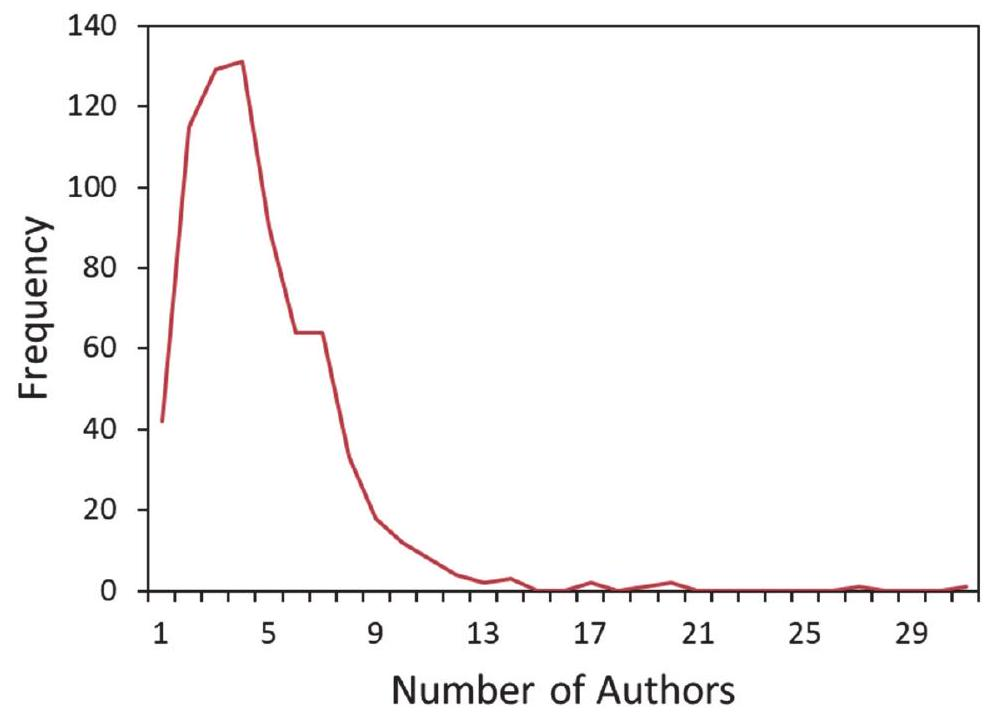
\includegraphics[max width=\textwidth]{2024_04_11_419211c3e451fc7cea07g-090}
\end{center}

Figure 13.1 Number of $\mathrm{JM}^{3}$ authors per paper, 2002-2011.

\subsection*{13.6 Conclusions}
Authorship is an important issue in the world of science. Reputations, even legacies, are often built on a history of publications. The two ethical principles of fairness and accountability are tied into the practice of assigning authorship for scientific papers. The definition of authorship proposed in this chapter, and the proper application of the proposed authorship test, can help ensure that authorship decisions contribute to, rather than detract from, the proper pursuit of science. Though I am sure that anyone determined enough can find or create a loophole to justify a predetermined authorship decision, following the spirit of this proposal should alleviate most concerns and conflicts regarding authorship.

Finally, I should note that standards of authorship are to a certain extent cultural, meaning that different communities (disciplines) of scientists set their own standards within the wider culture of science as a whole. The opinions I have expressed in this editorial reflect what I feel are the correct positions for the scientific communities I have been involved in. They may not be a perfect match to every discipline of science and engineering, though I suspect that they are not too far off for most scientific communities.

\section*{References}
${ }^{1} \mathrm{~V}$. Khachatryan et al., "First measurement of Bose-Einstein correlations in proton-proton

\begin{center}
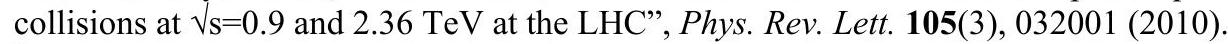
\includegraphics[max width=\textwidth]{2024_04_11_419211c3e451fc7cea07g-091}
\end{center}

${ }^{2}$ P. J. Wyatt, "Too many authors, too few creators", Physics Today 65(4), 9-10 (2012).

${ }^{3}$ D. Kamerow, "Who wrote that article?", Br. Med. J. 336(7651), 989 (2008).

${ }^{4}$ P. K. Baskin and R. A. Gross, "Honorary and ghost authorship", Br. Med. J. 343, d6223 (2001).

5 H. C. Polk, Jr., et al., "Consensus statement on submission and publication of manuscripts", J. Thorac. Cardiovasc. Surg. 121(6), 1029-1030 (2001).

${ }^{6}$ B. C. Martinson, M. S. Anderson, and R. de Vries, "Scientists behaving badly", Nature 435(7043), 737-738 (2005).

7 SPIE, "SPIE Code of Ethics", \href{http://spie.org/Documents/Publications/SPIE-Code-ofEthics.pdf}{http://spie.org/Documents/Publications/SPIE-Code-ofEthics.pdf}.

${ }^{8}$ National Research Council, "On being a scientist: responsible conduct in research, second edition", National Academies Press, Washington, DC (1995).

${ }^{9}$ G. N. Levy, "Surprise authorship", Science 275(5308), 1861-1865 (1997).

${ }^{10}$ A. Matheson, "How industry uses the ICMJE guidelines to manipulate authorship - and how they should be revised", PLoS Med. 8(8), 1001072 (2011).

11 "Policy on papers' contributors", Nature 399(6735), 393 (1999).

\section*{Chapter 14 Plagiarism}
Plagiarism remains a difficult and important issue in scientific publishing. SPIE, with its many peer-reviewed journals and conference proceeding publications, deals with a number of plagiarism cases each year, ranging from the minor (fixable with editing and education) to the major (sometimes requiring retraction and author sanctions). And even though copying is easier than ever to detect using automated tools such as Similarity Check, the problem persists.

Plagiarism is generally defined as taking another's ideas, images, or words and representing them as one's own. It is intellectual theft. Despite this seemingly clear definition, in my experience the practice of defining and identifying plagiarism is much more complicated and nuanced. Often, plagiarism is more a consequence of intellectual laziness than intellectual dishonesty. While I want to believe that everyone attempting to write and publish a scientific paper has the same ethical understanding of the concepts of plagiarism as I do, I know this is not the case. So, let us parse our definition of plagiarism and see how it applies to the practices of writing and publishing a scientific paper.

\subsection*{14.1 Copying Another's Ideas}
It is a bedrock principle of science that each new work builds on the foundation of past work, so that making use of another's ideas is not only allowed but encouraged. The ethical lapse comes from misrepresenting those ideas as one's own. Such misrepresentation can be explicit ("We present here for the first time...") but is most often implicit. By presenting ideas, designs, models, processes, or results without citations, there is a clear implication that these ideas are original. Thus, the plagiarism of ideas can also be considered a lapse in proper citation practices. The first defense against the plagiarism of ideas is to be very familiar with the right and wrong ways to cite prior work (see Chapter 5).

A missing citation is not necessarily evidence of plagiarism. After all, many ideas have been formulated independently by different people, and no one is familiar with all of the literature, even in narrow fields. Authors are expected to make a concerted effort to find relevant literature and cite appropriately, but missing citations are generally dealt with during the review and editing proces without any implications of wrongdoing. Partly this is due to the difficulty of proving the intent to inappropriately copy another's ideas.

\subsection*{14.2 Copying Another's Images}
Figures are an important part of scientific communication, and the generation of a figure or other image is generally a creative act. As such, the use of another's figure requires not only a reference to its original publication, but permission from the figure's author (and possibly the publisher) as well. Slight modifications to a figure (the equivalent of image "paraphrasing") are not enough to escape this requirement. Of course, some images have little or no creative content (block diagrams of a common experimental setup, for example), and present few options for a different representation. But thanks to the human brain's incredible ability to process images quickly and efficiently, it is generally safe to say that I know a copied image when I see one.

\subsection*{14.3 Copying Another's Words}
By far the most common plagiarism problem that I am forced to deal with as an editor is the copying of another's words. Writing well is hard work (see Chapter 3 ), and the reward for that work is often limited to the credit one receives for its publication. Thus, stealing words - taking the credit that rightly belongs to another - besides being inherently dishonest, can rob an author of the reward that may have justified the original effort.

The severity of an act of text copying can vary greatly, from the wholesale copying of an entire paper to the inadequate paraphrasing of a few sentences. While copying text (without quoting) is never allowed, the magnitude of the problem depends on several important factors:

\begin{itemize}
  \item Was the source of the copied text cited? The lack of a citation is considered evidence of an intent to deceive, as opposed to carelessness or poor writing practices.
  \item How many sentences were copied? The greater the amount of copying, the greater the offense.
  \item Was there paraphrasing, or merely an attempt to disguise copying? One can avoid plagiarism by proper paraphrasing. But slight changes to a word or two of a copied sentence are not the same as rewriting in your own words. Note that paraphrased passages still require a citation to the original.
  \item Is any of the copied text claimed to be a novel aspect of the paper? Copying limited to background material or the methods section is still plagiarism but not as egregious as the copying of results or their interpretation.
\end{itemize}

The last bullet point is worth exploring in more detail. Some authors seem to think copying text that merely describes the background of the field of study (i the Introduction section) or that describes an experimental procedure that is not new (in the Methods section) is somehow exempt from the rules against plagiarism. This is not true. If the words are not your own, then you are quoting someone else, and to quote someone else requires quotation marks (or indented text) and a citation.

\subsection*{14.4 Duplicate Publication, or Self-Plagiarism}
The term "self-plagiarism" is an oxymoron: you cannot steal from yourself. Still, the term is often used to describe a serious problem: misrepresenting previously published work as new. Such duplicate publication without proper citation is sometimes used by authors to increase their publication counts, hoping that editors and reviewers will not notice the lack of novelty in their latest submission. The harm here is to the journal and its readers, who waste their time reviewing and reading old work, thinking that there is something new to learn. Unlike a missing citation to someone else's work, authors cannot claim ignorance as an excuse for not citing their own prior work. Thus, duplicate publication is a serious ethical violation (see Chapter 15). Note that this is true for the Introduction and Method sections as well as for the Results and Discussion sections. If you copy your own text or figures, cite it (though you do not need to add quotation marks). If your new work is a continuation of your old work, cite it. Make sure the reader can easily distinguish between what is new and what is old.

Occasionally, there are also copyright issues related to the reuse of one's previously published words or images. It is the responsibility of the authors to ensure that the copyright agreement they signed with the prior publisher allows word or image reuse by those same authors in a new publication, or to obtain written permission if not.

The idea of copying and reusing your own text (with citation) becomes more complicated if the author lists of the new and old papers are not identical. You cannot steal your own words, but whose words are you taking when you copy from a paper that has some authors not found on the new manuscript? If the author list of the new paper does not include every author from the prior paper, text and ideas taken from that prior paper must be cited to give credit to the other authors of that work.

\subsection*{14.5 Cultural Issues}
It is not a coincidence that a disproportionate number of plagiarism cases at English-language scientific journals involve non-native English speakers. I am sure that the temptation to copy someone else's well-worded text rather than attempt rewriting it in one's own words must be strong when writing in English does not come easily. But I suspect that the most likely explanation for the higher incidence of plagiarism amongst foreign authors is cultural.

While the educational systems in countries such as China and India are changing rapidly, there is still a strong emphasis on rote memorization and

verbatim recitation as means of both learning and demonstrating learning. This i especially true when it comes to English-language source material, where exams often require the wholesale repetition of a textual source in order to get the answer "right". An educational system that requires the memorization and repetition of another's words in order to succeed does not prepare a student well for our academic ideals of intellectual originality and attribution.

That said, widely accepted practices of attribution and prohibitions of plagiarism are firmly embedded in the scientific community's publication practices. I hope that universities will actively teach these standards to all science students, especially during their first few publication experiences (usually as graduate students).

\subsection*{14.6 Conclusions}
The consequences of plagiarism for the authors depend on the severity of the ethical misconduct. The SPIE Code of Ethics has this to say about plagiarism and duplicate publication: ${ }^{1}$

There are varying degrees of plagiarism warranting different consequences and corrective action, listed below from most to least serious:

\begin{itemize}
  \item Verbatim or nearly verbatim copying or translation of a full paper(s), or the verbatim or nearly verbatim copying or translation of a significant portion(s) of another paper(s).
  \item Disclosing unpublished data or findings without permission, even if attributed.
  \item Uncredited verbatim or nearly verbatim copying or translation of individual elements of another paper(s).
  \item Uncredited paraphrasing of pages or paragraphs from another paper(s).
  \item Credited verbatim copying or translation of a major portion of a paper without clear delineation (e.g., quotes or indents).
\end{itemize}

The degree of corrective action will be commensurate with the degree of plagiarism.

If duplicate publication in peer-reviewed journals is suspected, the investigating/enforcing body will confirm this by assessing the similarity and determining the paper's publication history. An attempt will be made to coordinate corrective actions with the editor(s) of the other publication(s).

Sometimes, minor lapses in plagiarism standards caught during journal submission can be fixed during editing with nothing more than a warning to the authors. More serious cases almost always result in the rejection of the submitte manuscript. For the most egregious cases, where intent to deceive can be reasonably established, rejection can be accompanied by a ban on publishing for one to several years (or even a lifetime ban in some extreme cases). Except in very rare circumstances, authors are considered collectively responsible for their paper.

\section*{References}
${ }^{1}$ SPIE, "SPIE Code of Ethics", \href{http://spie.org/Documents/Publications/SPIE-Code-ofEthics.pdf}{http://spie.org/Documents/Publications/SPIE-Code-ofEthics.pdf}.

\section*{Chapter 15}
\section*{Double Publication}
Peer-reviewed journals almost always have a restriction against double publication - submitting for publication a manuscript that is substantially the same as one that has already been published by another peer-reviewed journal. A related concept (which is also prohibited) is double submission, where the same or substantially the same manuscript is under consideration for publication by two peer-reviewed journals simultaneously. At the Journal of Micro/Nanolithography, MEMS, and MOEMS $\left(\mathrm{JM}^{3}\right)$, for example, manuscript submission includes a requirement that the submitter acknowledge any prior publication of any of the major results/data/figures/etc. found in the submitted manuscript. But while submitting a manuscript that has already been published is an obvious problem, defining when duplicate content crosses the line to duplicate publication is not always easy. What, exactly, does "substantially the same" mean?

\subsection*{15.1 Something Old, Something New}
Among other criteria, a manuscript must contain something novel to make it publishable in a peer-reviewed scientific journal (see Chapter 7). But not everything discussed in a paper must be novel. It is common for a paper to begin by discussing prior (already published) results before moving on to what is new. It is the authors' responsibility to clearly differentiate between prior work and new results. This can be done explicitly through direct language ("Prior work has shown..."; "In this work, we measured...") or implicitly though the use of citations. Statements that end in a citation are understood to be descriptions of prior work. Conversely, statements of results without citations are generally assumed to be novel, presented in the paper for the first time.

This is where authors sometimes get themselves into trouble. Sloppy citation practice can lead to an assumption on the part of the reader (or editor or reviewer) that prior work is being claimed as something novel in this new work. And while most authors are reasonably careful about not making such a mistake when it comes to other people's prior work (thus avoiding implications of plagiarism, see Chapter 14), they are often much less careful when citing their own prior work. "Who does it harm," the thought goes, "if I fail to cite my own prior work?"

Two harms result from the absence of necessary self-citations. First, because the exact author lists of the previous and new paper are often different, failure to cite prior work that is re-presented in a new paper will often leave someone with too much or too little credit. Second, failing to cite one's prior work could be viewed as an implicit (and undeserved) claim of novelty.

Which brings us back to the topic of double publication. My rule of thumb is that at least $50 \%$ of the major results/data/figures/etc. found in a manuscript submitted to a peer-reviewed journal must be novel to permit publication. This is just a guideline, however, and depends somewhat on the significance of the new results. Obviously, having the new material clearly distinguishable from the old is a requirement for assessing whether a submitted manuscript presents new science or is "substantially the same" as one or more prior publications. It is a serious ethical lapse to purposely leave out citations to one's own prior work in order to try to pass off a substantially duplicate paper as something new.

In summary, proper citations are necessary for many reasons (see Chapter 5), not the least of which is to distinguish what is novel in the paper. The criteria for proper citations do not depend on whether the prior work is your own or someone else's, or whether the prior work was published in a peer-reviewed journal, conference proceedings, or some alternate publication medium. Sloppy citation practice veers into citation malpractice when leaving off a citation helps to induce an editor (or reviewer or reader) to believe that something old is something new.

\subsection*{15.2 The Role of Conference Proceedings}
Let me repeat my definition of double publication: submitting for publication a manuscript that is substantially the same as one that has already been published by another peer-reviewed journal. The last constraint, that only peer-reviewed publications are considered when evaluating double publication, is not universally adopted in scientific publishing. Some journals are far more restrictive, banning duplicate content from conference proceedings, conference abstracts, website postings, or even press releases.

SPIE has a fairly lenient policy about submitting the content of conference proceedings papers to one of its peer-reviewed journals. The reason is simple: SPIE recognizes the important and unique role of conferences, and their proceedings, in the growth of scientific knowledge as complementary to the important role of peerreviewed journals. Our philosophy is that conferences and journals should work together rather than in competition. Conference proceedings provide a record of the conference, a snapshot in time of a rapidly developing field of science or engineering. Peer-reviewed journals provide an asynchronous look at a completed effort (or at least a milestone in a larger effort), carefully presented to provide lasting value to the scientific community.

Because both types of publications are important, SPIE allows previously published conference papers to be submitted, in whole or in part, to an SPIE peerreviewed journal, given that certain criteria are met. Not all journals have such a policy, and it is important to investigate the details of what counts as doubl publication at the specific journal you wish to submit to. In all cases, citation of the prior conference proceedings is required.

\subsection*{15.3 Conclusions}
Unfortunately, journal editors sometimes have to deal with the problem of double publication. Occasionally, the problem is unintentional, the result of sloppy citations and lack of consideration of the topic. Frequently, though, authors are trying to inflate their publication counts by spreading a body of work too thin and over too many papers. I hope that authors will take the lessons of this chapter seriously, and editors will have to deal with fewer and fewer of these issues over time.

\section*{Chapter 16 Editorial Ethics}
Several chapters of this book have touched on the ethical responsibilities of the authors: how to properly cite the work of others (Chapter 5), how to determine who belongs on the list of authors (Chapter 13), and how to avoid plagiarism (Chapter 14) and double publication (Chapter 15), among other topics (Chapter 12). But in the peer-review process, authors are not the only ones with ethical responsibilities. Editors and reviewers have important obligations as well. In Chapter 10, I briefly described the responsibilities of the authors, editors, and reviewers. Here, I will go into more detail on the ethical responsibilities of editors.

\subsection*{16.1 Editors' Responsibilities}
Although there are many ways to summarize the ethical duties of the editors of a peer-reviewed scientific journal, the following is a list of seven items that I think covers the main points:

\begin{enumerate}
  \item Provide a transparent process for editorial review, and deviate from that process only under exceptional circumstances.
\end{enumerate}

As an example of transparency, Chapter 10 describes the Journal of Micro/Nanolithography, MEMS, and MOEMS $\left(\mathrm{JM}^{3}\right)$ editorial process in detail. To my knowledge, we have not deviated from that process since its publication in 2015. While tweaks to this process are likely to occur in the future, $\mathrm{JM}^{3}$ will publish any noteworthy changes when needed.

\begin{enumerate}
  \setcounter{enumi}{1}
  \item Deal fairly and respectfully with all parties in the publishing process.
\end{enumerate}

Editors and publishers should be committed to fair and respectful treatment of both authors and reviewers, and expect the same from authors and reviewers in their treatment of editors and staff. Any behavior that does not rise to the highest standards should be reported to the editor-in-chief and/or to the publisher.

\begin{enumerate}
  \setcounter{enumi}{2}
  \item Recuse yourself when dealing with a manuscript for which you have a conflict of interest-let a non-conflicted editor handle the submission and make the decisions.
\end{enumerate}

Some conflicts are easy to recognize, such as when one or more of the authors works for the same company/organization as the editor. Other conflicts are not so clear-cut, as when the editor feels a competitive threat (commercially or professionally) from the work being submitted or has a strong personal tie to an author. I rely on my editors to honestly assess their own potential conflicts and to discuss with me any questionable cases.

\section*{4. Ensure that all details of a submission are kept confidential.}
The software systems used to manage manuscripts through the submission, review, and publication process typically provide a standard level of security to ensure confidentiality. Beyond that, journals should instruct all of their editors to keep all information about a manuscript and its reviews and revisions confidential within the board of editors and publisher. Only after a paper has been published can the contents of that paper be discussed outside the editorial board. Even then, only published information can be discussed, with the details of reviews or revisions to remain confidential unless the authors decide to release them.

As an aside, many editors, myself included, submit manuscripts to the journals they are involved with. When an editor is an author of a submission, the manuscript is handled by other editors in such a way that the editor-author remains completely outside the review and decision process. In my case, any information about a manuscript I submit, including who is assigned as the associate editor and who performs the reviews, is redacted from the internal database we use to track manuscripts so that I cannot view such details (even if I am tempted to peek). I have submitted many papers to $\mathrm{JM}^{3}$ since I became editor-in-chief, and never once has this wall of confidentiality been breached.

\begin{enumerate}
  \setcounter{enumi}{4}
  \item Work assiduously for timely decisions.
\end{enumerate}

Everyone wants the publication process to be speedy. At $\mathrm{JM}^{3}$, the median time from receipt of a manuscript to the first editorial decision was 10 weeks in 2008, but only 5 weeks in 2016 . Unfortunately, some manuscripts take much longer, either because it is very hard to find reviewers or the reviewers are late in supplying their reviews. Sometimes delays are caused by editors who do not perform their duties quickly (our volunteer editors tend to be very busy people), but we continue to try to improve our performance in this regard. At the back end, the median time from acceptance to publication was 3.4 weeks in 2016 (down from 14 weeks in 2008), due to the time required for copyediting, typesetting, and the somewhat variable time for author page-proof review. Technological changes have greatly sped up this last step.

\begin{enumerate}
  \setcounter{enumi}{5}
  \item Choose reviewers who are likely to provide fair, unbiased, high-quality, and timely reviews.
\end{enumerate}

Generally, editors have been chosen for their knowledge in important fields covered by the scope of the journal. In many cases, a manuscript covers a familia topic, and the editor responsible for handling the submission can seek reviewers who are known to be unbiased experts. In other cases, we may have to deal with reviewers we do not personally know. An editor's greatest frustration is nonresponsive reviewers (either because they do not respond to a request to become a reviewer or they do not submit their review on time after agreeing to review). I am not sure how to solve this problem, other than asking reviewers to treat the process the way they wish to be treated as authors.

\begin{enumerate}
  \setcounter{enumi}{6}
  \item Hold all parties in the publishing process to the highest ethical standards.
\end{enumerate}

$\mathrm{JM}^{3}$ is a member of COPE, the Committee on Publication Ethics. As such, I am committed to following the COPE code of conduct for journal editors. ${ }^{1}$ This code of conduct describes the basic principles of serving the needs of both authors and readers with integrity while promoting our journal's mission of furthering scientific knowledge.

\subsection*{16.2 Conclusions}
Editors, reviewers, and authors work together with the shared goal of furthering science through the publication process. The best results come when these parties work together in a spirit of mutual respect and cooperation, keeping the reader as the center of their concern. As such, each of these players has ethical responsibilities to the others. While most of this book has been focused on authors and what they need to keep in mind when writing a good scientific paper, it is useful to remind editors of their ethical responsibilities as well.

\section*{References}
\footnotetext{${ }^{1}$ Committee on Publication Ethics, "Code of Conduct and Best Practice Guidelines for Journal Editors", version 4 (2011).
}

\section*{Appendix}
\section*{A Checklist for Editors, Reviewers, and Authors}
\section*{Should the manuscript be rejected?}
Reject the manuscript if one or more of the answers to the following questions is no. Support all no answers with specific reasons.

\begin{itemize}
  \item Does the content of the manuscript match the scope of the journal?
\end{itemize}

If no: Is there a journal with a better match?

\begin{itemize}
  \item Does the manuscript present novel results (with the exception of review papers and the like)?
\end{itemize}

If no: Did the author(s) fail to distinguish what was novel? Where was similar content published?

\begin{itemize}
  \item Are the results significant enough to be worth reading about (and thus worth publishing)? Will it impact the thoughts or actions of its readers?
\end{itemize}

If no: Is it possible to increase the significance with more data, different analysis, improved theoretical treatment, etc.? Would a different audience (different journal) find the work more significant?

\begin{itemize}
  \item Do the data support the conclusions (i.e., is the quality of the research sufficiently high)?
\end{itemize}

If no: Can the conclusions be scaled back to what the data allow, and if so, would the results still be significant? Is it possible to add more data/theoretical treatment/etc. to enable the conclusions to be supported?

\begin{itemize}
  \item Is the writing of sufficient quality to allow the above points to be evaluated?
\end{itemize}

If no: What suggestions would help the author(s) get the manuscript in better shape (e.g., English-language editing, better organization, etc.)?

\section*{If the manuscript is not rejected, what should be changed to make it acceptable for publication?}
Reviewers can use the following checklist as a guide for creating a comprehensive review of the work, with suggestions for improvements. For authors, asking the questions and following the instructions below will result in a paper more likely to be accepted for publication.

\section*{Organization, Length, and Clarity}
\begin{itemize}
  \item Is the work well-organized and structured so that conclusions logically follow from results that logically follow from the methods used? Do those conclusions answer the research questions initially posed?
  \item Make sure the length of the manuscript is appropriate. Does the knowledge gained by the reader justify the time spent reading?
  \item Is the thought process clear? Is clear language used (claiming neither more nor less than can be justified)?
\end{itemize}

\section*{Introduction}
\begin{itemize}
  \item Indicate the field of the work, why this field is important, and what has already been done (with proper citations).
  \item Indicate a gap, raise a research question, or challenge prior work in this territory.
  \item Outline the purpose and announce the present research, clearly indicating what is novel and why it is significant.
  \item Avoid: repeating the abstract; providing unnecessary background information; exaggerating the importance of the work; claiming novelty without a proper literature search.
\end{itemize}

\section*{Method (Materials, Theory, Design, Modeling, etc.)}
\begin{itemize}
  \item Describe how the results were generated with sufficient detail so that an independent researcher (working in the same field) could reproduce the results sufficiently to allow validation of the conclusions.
  \item Can the reader assess internal validity (conclusions are supported by the results presented)?
  \item Can the reader assess external validity (conclusions are properly generalized beyond these specific results)?
  \item Has the chosen method been justified?
  \item Are data analysis and statistical approaches justified, with assumptions and biases considered?
  \item Avoid: including results in the Method section; including extraneous details (unnecessary to enable reproducibility or judge validity); treating the method as a chronological history of events; unneeded references to commercial products; references to "proprietary" products or processes unavailable to the reader.
\end{itemize}

\section*{Results and Discussion}
\begin{itemize}
  \item Present the results of the paper, in logical order, using tables and graphs as necessary.
  \item Explain the results and show how they help to answer the research questions posed in the Introduction. Evidence does not explain itself; the results must be presented and then explained.
  \item Typical stages in the discussion: summarizing the results, discussing whether results are expected or unexpected, comparing these results to previous work, interpreting and explaining the results (often by comparison to a theory or model), and hypothesizing about their generality.
  \item Discuss any problems or shortcomings encountered during the course of the work.
  \item Discuss possible alternate explanations for the results.
  \item Avoid: presenting results that are never discussed; presenting discussion that does not relate to any of the results; presenting results and discussion in chronological order rather than logical order; ignoring results that do not support the conclusions; drawing conclusions from results without logical arguments to back them up.
\end{itemize}

\section*{Conclusions}
\begin{itemize}
  \item Provide a very brief summary of the Results and Discussion.
  \item Emphasize the implications of the findings, explaining how the work is significant and providing the key message(s) the author wishes to convey.
  \item Provide the most general claims that can be supported by the evidence.
  \item Provide a future perspective on the work.
  \item Avoid: repeating the abstract; repeating background information from the Introduction; introducing new evidence or new arguments not found in the Results and Discussion; repeating the arguments made in the Results and Discussion; failing to address all of the research questions set out in the Introduction.
\end{itemize}

\section*{Acronyms}
\begin{itemize}
  \item The title should not use acronyms unless (a) the subject is almost exclusively known by its acronym or is widely known and used in that form, and (b) the acronym does not commonly have more than one expansion.
  \item Always spell out the acronym the first time it is used in the body of the paper.
  \item Avoid acronyms in the abstract unless the acronym is commonly understood and used multiple times in the abstract. If an acronym is used in the abstract, it must be spelled out (defined) in the abstract, and then spelled out again the first time it is used in the body of the paper.
\end{itemize}

\section*{Citations (References)}
\begin{itemize}
  \item Include citations that provide sufficient context to allow for critical analysis of this work by others.
  \item Include citations that give the reader sources of background and related material so that the current work can be understood by the target audience.
  \item Include citations that provide examples of alternate ideas, data, or conclusions to compare and contrast with this work, if they exist. Do not exclude contrary evidence.
  \item Include citations that acknowledge and give credit to sources relied upon for this work.
  \item Are the citations up to date, referencing that latest work on this topic?
  \item It is the job of the authors to verify the accuracy of the references.
  \item Avoid: spurious citations (citations that are not needed but are included anyway); biased citations (references added or omitted for reasons other than meeting the above goals of citations); excessive self-cites (citations to one's own work).
\end{itemize}

\section*{Figures and Tables}
\begin{itemize}
  \item Ensure that the figures accurately and carefully document the data and their context.
  \item Ensure that the figures allow for comparisons and inferences of cause and effect, avoiding spurious readings.
  \item Figures should have captions and legends to allow them to be understood independent of the text, if possible.
  \item Ideally, a figure caption will do three things: describe everything in the graph, draw attention to its important features, and (when practical) describe the main conclusions to be drawn from it.
  \item All figures should be referred to in the text, with first references in numerical order.
  \item A piece of data has four parts: a description (what is it?), a number, a unit, and an uncertainty estimate. Try to put all four parts of the data in the figure.
  \item Error bars should be present; explain clearly what they represent. If any data points have been removed, explain why.
  \item Use color when it can enhance the graphic (most articles are now read online), but make sure that no information is lost when printed in black and white.
  \item Tables are best for looking up specific information or exact values, and graphs excel at displaying trends and making comparisons.
  \item When the number of data points is small, a table could work better than a graph.
  \item Use log-scales to reveal trends in the data, not hide them. Log-scales emphasize relative changes, whereas linear scales are best at showing absolute changes.
  \item Choose plot scales ( $x$ - and $y$-axis start and stop values, for example) to avoid white space: try to use at least $80 \%$ of each scale to display data.
  \item Avoid: titles on the graph (title information should be in the figure caption); pie charts; bar charts unless there isn't a better option; spurious 3D effects, such as the use of 3D bars in a bar chart; gridlines and other clutter; inconsistent formatting of figures; commercial displays in the guise of diagrams or figures.
\end{itemize}

\section*{Abstract}
\begin{itemize}
  \item The abstract should be a concise (200 words or less), standalone summary of the paper, with 1-2 sentences on each of these topics:
\end{itemize}

○ Background: What issues led to this work? What is the environment that makes this work interesting or important?

Aim: What were the goals of this work? What gap is being filled?

Approach: What went into trying to achieve the aims (e.g., experimental method, simulation approach, theoretical approach, combinations of these, etc.)? What was actually done?

Results: What were the main results of the study (including numbers, if appropriate)?

Conclusions: What were the main conclusions? Why are the results important? Where will they lead?

\begin{itemize}
  \item The abstract should be written for the audience of this journal: do not assume too much or too little background with the topic.
  \item Ensure that all of the information found in the abstract also can be found in the body of the paper.
  \item Ensure that the important information of the paper is found in the abstract.
  \item Avoid: using the first paragraph of the introduction as an abstract; citations in the abstract; acronyms (but if used, spell them out); referring to figures or tables from the body of the paper; use of the first person; use of words like "new" or "novel," or phrases like "in this paper," "we report," or "will be discussed."
\end{itemize}

Title

\begin{itemize}
  \item The title should be clear and informative, and should reflect the aim and approach of the work.
  \item The title should be as specific as possible while still describing the full range of the work. Does the title, seen in isolation, give a full yet concise and specific indication of the work reported?
  \item Do not mention results or conclusions in the title.
  \item Avoid: overly clever or punny titles that will not fare well with search engines or international audiences; titles that are too short to be descriptive or too long to be read; jargon, acronyms, or trademarked terms.
\end{itemize}
